% Options for packages loaded elsewhere
\PassOptionsToPackage{unicode}{hyperref}
\PassOptionsToPackage{hyphens}{url}
\PassOptionsToPackage{dvipsnames,svgnames*,x11names*}{xcolor}
%
\documentclass[
]{book}
\usepackage{lmodern}
\usepackage{amssymb,amsmath}
\usepackage{ifxetex,ifluatex}
\ifnum 0\ifxetex 1\fi\ifluatex 1\fi=0 % if pdftex
  \usepackage[T1]{fontenc}
  \usepackage[utf8]{inputenc}
  \usepackage{textcomp} % provide euro and other symbols
\else % if luatex or xetex
  \usepackage{unicode-math}
  \defaultfontfeatures{Scale=MatchLowercase}
  \defaultfontfeatures[\rmfamily]{Ligatures=TeX,Scale=1}
\fi
% Use upquote if available, for straight quotes in verbatim environments
\IfFileExists{upquote.sty}{\usepackage{upquote}}{}
\IfFileExists{microtype.sty}{% use microtype if available
  \usepackage[]{microtype}
  \UseMicrotypeSet[protrusion]{basicmath} % disable protrusion for tt fonts
}{}
\makeatletter
\@ifundefined{KOMAClassName}{% if non-KOMA class
  \IfFileExists{parskip.sty}{%
    \usepackage{parskip}
  }{% else
    \setlength{\parindent}{0pt}
    \setlength{\parskip}{6pt plus 2pt minus 1pt}}
}{% if KOMA class
  \KOMAoptions{parskip=half}}
\makeatother
\usepackage{xcolor}
\IfFileExists{xurl.sty}{\usepackage{xurl}}{} % add URL line breaks if available
\IfFileExists{bookmark.sty}{\usepackage{bookmark}}{\usepackage{hyperref}}
\hypersetup{
  pdftitle={Introductory Mathematics for Economists with Matlab},
  pdfauthor={Fan Wang},
  colorlinks=true,
  linkcolor=Maroon,
  filecolor=Maroon,
  citecolor=Blue,
  urlcolor=blue,
  pdfcreator={LaTeX via pandoc}}
\urlstyle{same} % disable monospaced font for URLs
\usepackage{longtable,booktabs}
% Correct order of tables after \paragraph or \subparagraph
\usepackage{etoolbox}
\makeatletter
\patchcmd\longtable{\par}{\if@noskipsec\mbox{}\fi\par}{}{}
\makeatother
% Allow footnotes in longtable head/foot
\IfFileExists{footnotehyper.sty}{\usepackage{footnotehyper}}{\usepackage{footnote}}
\makesavenoteenv{longtable}
\usepackage{graphicx}
\makeatletter
\def\maxwidth{\ifdim\Gin@nat@width>\linewidth\linewidth\else\Gin@nat@width\fi}
\def\maxheight{\ifdim\Gin@nat@height>\textheight\textheight\else\Gin@nat@height\fi}
\makeatother
% Scale images if necessary, so that they will not overflow the page
% margins by default, and it is still possible to overwrite the defaults
% using explicit options in \includegraphics[width, height, ...]{}
\setkeys{Gin}{width=\maxwidth,height=\maxheight,keepaspectratio}
% Set default figure placement to htbp
\makeatletter
\def\fps@figure{htbp}
\makeatother
\setlength{\emergencystretch}{3em} % prevent overfull lines
\providecommand{\tightlist}{%
  \setlength{\itemsep}{0pt}\setlength{\parskip}{0pt}}
\setcounter{secnumdepth}{5}
\usepackage{bbm}
\usepackage{booktabs}
\usepackage{longtable}
\usepackage{array}
\usepackage{multirow}
\usepackage{wrapfig}
\usepackage{float}
% \floatplacement{figure}{H}
\usepackage[labelformat = empty]{caption}
\usepackage{colortbl}
\usepackage{pdflscape}
\usepackage{tabu}
\usepackage{threeparttable}
\usepackage{threeparttablex}
\usepackage[normalem]{ulem}
\usepackage{makecell}
\usepackage{xcolor}
\usepackage{geometry}
\geometry{
	a4paper,
	left=1.0in,
	right=1.0in,
	top=1.0in,
	bottom=1.0in,
}
\setcounter{secnumdepth}{5}
\setcounter{tocdepth}{5}
\usepackage[]{natbib}
\bibliographystyle{apalike}

\title{Introductory Mathematics for Economists with Matlab}
\author{Fan Wang}
\date{2020-05-31}

\begin{document}
\maketitle

{
\hypersetup{linkcolor=}
\setcounter{tocdepth}{1}
\tableofcontents
}
\hypertarget{preface}{%
\chapter*{Preface}\label{preface}}
\addcontentsline{toc}{chapter}{Preface}

This is a work-in-progress \href{https://fanwangecon.github.io/Math4Econ/}{course website} for Mathematics for Economists, produced by \href{https://fanwangecon.github.io/}{Fan}. Course covers a limited subset of topics from \href{Mathematics\%20for\%20Economists}{Mathematics for Economists} \citep{simonblume1994}, and uses various definitions from the book. Applications focus on two period borrowing and savings problems. Matlab's symbolic toolbox is used throughout.

Materials are written in \href{https://www.mathworks.com/products/matlab.html}{matlab} \citep{matlab} livescript files and shown as HTML files. To obtain matlab codes, see \href{docs/gitsetup.md}{here} and \href{docs/gitsetupown.md}{here} for github set up. For HTML files, click on the links below.

From \href{https://fanwangecon.github.io/}{Fan}'s other repositories: For dynamic borrowing and savings problems, see \href{https://fanwangecon.github.io/CodeDynaAsset/}{Dynamic Asset Repository}; For code examples, see also \href{https://fanwangecon.github.io/R4Econ/}{R Example Code}, \href{https://fanwangecon.github.io/M4Econ/}{Matlab Example Code}, and \href{https://fanwangecon.github.io/Stata4Econ/}{Stata Example Code}; For intro econ with Matlab, see \href{https://fanwangecon.github.io/Math4Econ/}{Intro Mathematics for Economists}. See \href{https://github.com/FanWangEcon}{here} for all of \href{https://fanwangecon.github.io/}{Fan}'s public repositories.

The site is built using \href{https://bookdown.org/}{Bookdown} \citep{R-bookdown}.

Please contact \href{https://fanwangecon.github.io/}{FanWangEcon} for issues or problems.

\hypertarget{notations-and-functions}{%
\chapter{Notations and Functions}\label{notations-and-functions}}

\hypertarget{real-number-and-intervals}{%
\section{Real Number and intervals}\label{real-number-and-intervals}}

\begin{quote}
Go back to \href{http://fanwangecon.github.io/}{fan}'s \href{https://fanwangecon.github.io/CodeDynaAsset/}{CodeDynaAsset} Package, \href{https://fanwangecon.github.io/M4Econ/}{Matlab Code Examples} Repository (\href{https://fanwangecon.github.io/M4Econ/bookdown}{bookdown site}), or \href{https://fanwangecon.github.io/Math4Econ/}{Math for Econ with Matlab} Repository (\href{https://fanwangecon.github.io/Math4Econ/bookdown}{bookdown site}).
\end{quote}

\hypertarget{real-number-line}{%
\subsection{Real Number Line}\label{real-number-line}}

\({{R^1 }}\) : can write \(R^1\) or \(R\) (you can add a superscript 1 to
emphasize this is first Euclidean space, either notation is fine), is
the real number line.

\begin{verbatim}
close all;
figure();
x = linspace(-10,10);
line(x,0*ones(size(x)))
set(gca,'ytick',[],'Ycolor','w','box','off')
ylim([-0.1 0.1])
pbaspect([4 1 1])
grid on
\end{verbatim}

\includegraphics[width=5.20833in,height=\textheight]{_img/realnumber_images/figure_0.png}

\hypertarget{non-negative-numbers}{%
\subsection{Non-negative numbers}\label{non-negative-numbers}}

In many economic problems, we have to restrict ourselves to numbers
greater or equal to zero.

\begin{itemize}
\item
  We can not consume from negative numbers of apples
\item
  We can not produce with negative labor and capital
\item
  We would be infinitely unhappy (die) if there is zero consumption in
  a year
\end{itemize}

We can use the following notation to define the set of non-negative real
numbers:

\({{R_{\ge 0} }}\equiv \lbrace x\in {R}:x\ge 0\rbrace\), some authors use
\({{R_+ }}\) instead of \({{R_{\ge 0} }}\)

And use inequality sign to define the set of real numbers greater than
zero:

\({{R_{>0} }}\equiv \lbrace x\in {R}:x>0\rbrace\), some authors use
\({{R_{++} }}\) instead of \({{R_{>0} }}\)

\begin{verbatim}
close all;
figure();
x = linspace(0,10);
line(x,0*ones(size(x)))
set(gca,'ytick',[],'Ycolor','w','box','off')
ylim([-0.1 0.1])
xlim([-10 10])
pbaspect([4 1 1])
grid on
\end{verbatim}

\includegraphics[width=5.20833in,height=\textheight]{_img/realnumber_images/figure_1.png}

\vspace{1em}

\hypertarget{interval-notations-and-examples}{%
\section{Interval Notations and Examples}\label{interval-notations-and-examples}}

\begin{quote}
Go back to \href{http://fanwangecon.github.io/}{fan}'s \href{https://fanwangecon.github.io/CodeDynaAsset/}{CodeDynaAsset} Package, \href{https://fanwangecon.github.io/M4Econ/}{Matlab Code Examples} Repository (\href{https://fanwangecon.github.io/M4Econ/bookdown}{bookdown site}), or \href{https://fanwangecon.github.io/Math4Econ/}{Math for Econ with Matlab} Repository (\href{https://fanwangecon.github.io/Math4Econ/bookdown}{bookdown site}).
\end{quote}

When we look at the problem facing a household, we often have to
restrict the choice set for example to an interval.

\hypertarget{closed-interval}{%
\subsection{Closed Interval}\label{closed-interval}}

For example, if \(x\) is hours working, perhaps the household has to work
at least \(a\) hours and up to \(b\) hours, so his choice is between \(a\) and
\(b\) hours inclusive.

The interval that is inclusive of both endpoints is called a closed
interval (note the square brackets):

\begin{itemize}
\tightlist
\item
  \textbf{closed interval}:
  \(\left\lbrack a,b\right\rbrack \equiv \lbrace x\in {R}:a\le x\le b\rbrace\)
\end{itemize}

\hypertarget{open-interval}{%
\subsection{Open Interval}\label{open-interval}}

In general, an open interval is defined as (Note here we use
parenthesis, not square brackest) :

\begin{itemize}
\tightlist
\item
  \textbf{open
  interval}:\(\left(a,b\right)\equiv \lbrace x\in {R}:a<x<b\rbrace\)
\end{itemize}

\hypertarget{half-open-and-half-close-interval}{%
\subsection{Half Open and Half Close Interval}\label{half-open-and-half-close-interval}}

We can also hafl half open intervals:

\begin{itemize}
\item
  \textbf{half open (half closed) interval}:
  \(\left\lbrack a,b\right)\equiv \lbrace x\in {R}:a\le x<b\rbrace\)
\item
  \textbf{half open (half closed) interval}:
  \(\left(a,b\right\rbrack \equiv \lbrace x\in {R}:a<x\le b\rbrace\)
\end{itemize}

\hypertarget{graph}{%
\subsection{Graph}\label{graph}}

If you were to graph an interval, you can draw an empty circle at either
end of an interval that is open, and a solid circle if it is closed at
that end.

\begin{verbatim}
close all;
figure();
x = linspace(-1,5);
line(x,0*ones(size(x)))
set(gca,'ytick',[],'Ycolor','w','box','off')
ylim([-0.1 0.1])
xlim([-10  10])
pbaspect([4 1 1])
grid on
\end{verbatim}

\includegraphics[width=5.20833in,height=\textheight]{_img/interval_images/figure_0.png}

\vspace{1em}

\hypertarget{what-is-a-function}{%
\section{What is a Function?}\label{what-is-a-function}}

\begin{quote}
Go back to \href{http://fanwangecon.github.io/}{fan}'s \href{https://fanwangecon.github.io/CodeDynaAsset/}{CodeDynaAsset} Package, \href{https://fanwangecon.github.io/M4Econ/}{Matlab Code Examples} Repository (\href{https://fanwangecon.github.io/M4Econ/bookdown}{bookdown site}), or \href{https://fanwangecon.github.io/Math4Econ/}{Math for Econ with Matlab} Repository (\href{https://fanwangecon.github.io/Math4Econ/bookdown}{bookdown site}).
\end{quote}

\textbf{function/mapping}: a mapping (also called a function) is a rule that
assigns to every element x of a set X a single element of a set Y. It is
written as:

\[f:X\to Y\]

where the arrow indicates mapping, and the letter \(f\) symbolically
specifies a rule of mapping. When we write:

\[y=f(x)\]

we are mapping from argument \(x\) in domain \(X\) to value \(y\) in co-domain
Y.

\textbf{\emph{Definitions:}}

\begin{itemize}
\item
  \textbf{domain}: big \(X\) is the domain of \(f\)
\item
  \textbf{argument}: little \(x\) is an element in big \(X\), an argument of
  the function \(f\).
\item
  \textbf{co-domain}: big \(Y\) is the co-domain of \(f\).
\item
  \textbf{image/value}: when \(y=f(x)\), we refer to \(y\) as the image or
  value of \(x\) under \(f\).
\item
  \textbf{range}:
  \(f(X)=\lbrace y\in Y:y=f(x)\;\textrm{for}\;\textrm{some}\;x\in X\rbrace\)
\end{itemize}

In some textbooks, \(x\) is called independent or exogenous variables, and
\(y\) is called dependent or endogenous variables. We will avoid using
those words to avoid confusion.

\textbf{\emph{This is a function}}:

\begin{verbatim}
figure();
x = 0:pi/100:2*pi;
y = sin(x);
plot(x,y);
grid on;
\end{verbatim}

\includegraphics[width=5.20833in,height=\textheight]{_img/whatisfunction_images/figure_0.png}

\textbf{\emph{This is NOT a function}}:

\begin{verbatim}
figure();
x = 1; y=1; r=1;
th = 0:pi/50:2*pi;
xunit = r * cos(th) + x;
yunit = r * sin(th) + y;
h = plot(xunit, yunit);
grid on;
\end{verbatim}

\includegraphics[width=5.20833in,height=\textheight]{_img/whatisfunction_images/figure_1.png}

\hypertarget{function-notations}{%
\section{Function Notations}\label{function-notations}}

\begin{quote}
Go back to \href{http://fanwangecon.github.io/}{fan}'s \href{https://fanwangecon.github.io/CodeDynaAsset/}{CodeDynaAsset} Package, \href{https://fanwangecon.github.io/M4Econ/}{Matlab Code Examples} Repository (\href{https://fanwangecon.github.io/M4Econ/bookdown}{bookdown site}), or \href{https://fanwangecon.github.io/Math4Econ/}{Math for Econ with Matlab} Repository (\href{https://fanwangecon.github.io/Math4Econ/bookdown}{bookdown site}).
\end{quote}

When you read your first economic papers, perhaps you are confused about
function notation. Economic models include potentially a lot of
variables, and different notations are used based on personal
preference. Make sure you use consistent notations, and state clearly
what your notations mean.

In general, the letter \(f\) represents a particular rule of mapping, if
there are multiple functional relationships in an economic model,
different letters could be used, for example:

\[y=f(h),l=g(h),u=w(h)\]

These three equations could be from a model where:

\begin{itemize}
\item
  \(h\) is the number of hours an individual works
\item
  \(y\) is the income that the individual makes as a function of work
  hours
\item
  \(l\) is the number of leisure hours remaining as a function work
  hours
\item
  \(u\) is the overall level of utility as a function of work hours.
\end{itemize}

Sometimes we have to write down many functions, and we can potentially
run out of letters. Hence, you might potentially want to use
superscripts:

\[y=f^y (h),l=f^l (h),u=f^w (h)\]

or we could use the same letter for function as the letter for the value
of the function, although this could be confusing because the function
mapping would have the same notation as a value of the function:

\[y=y(h),l=l(h),u=u(h)\]

if the above notation seems unclear, you can perhaps use more cursive
letters for functions, latex offers different fonts/typesetting options:

\[y=\mathcal{y}(h),l=\mathcal{l}(h),u=\mathcal{u}(h)\]

Again, make sure you are clear about what your notations mean. Math
should help make our econ ideas more clear to ourselves and others, and
that starts with clear functional notations.

\hypertarget{monomial-and-polynomial}{%
\section{Monomial and Polynomial}\label{monomial-and-polynomial}}

\begin{quote}
Go back to \href{http://fanwangecon.github.io/}{fan}'s \href{https://fanwangecon.github.io/CodeDynaAsset/}{CodeDynaAsset} Package, \href{https://fanwangecon.github.io/M4Econ/}{Matlab Code Examples} Repository (\href{https://fanwangecon.github.io/M4Econ/bookdown}{bookdown site}), or \href{https://fanwangecon.github.io/Math4Econ/}{Math for Econ with Matlab} Repository (\href{https://fanwangecon.github.io/Math4Econ/bookdown}{bookdown site}).
\end{quote}

\hypertarget{monomial}{%
\subsection{Monomial}\label{monomial}}

Functions of the form:

\[a\cdot x^k\]

are monomials.

\begin{itemize}
\item
  \(a\) is any real number, it is the coefficient.
\item
  \(k\) is a positive integer, it is the degree of the monomial
\end{itemize}

\hypertarget{polynomial}{%
\subsection{Polynomial}\label{polynomial}}

Monomials added up together are polynomials

\[a+b\cdot x+c\cdot x^2 +d\cdot x^3 +e\cdot x^4\]

The coefficients \(a,b,c,d,e\) above could be positive or negative.

\begin{itemize}
\tightlist
\item
  \textbf{Degree of Polynomial}: We say that this polynomial has degree
  of 4. You find the largest degree monomial in the polynomial, and
  its degree is the degree of the whole polynomial.
\end{itemize}

\hypertarget{graphical-monomial-examples}{%
\subsection{Graphical Monomial Examples}\label{graphical-monomial-examples}}

Take a look at the function below, matlab makes it very easy to plot
functions. You can see that when we shift the coefficient for the
monomial, it rescales the function but does not change the ordinality.

Monomial when a = 0.75, a = 1, and a = 1.25:

\begin{verbatim}
clear all;
a = 0.75;
monomial_graph(a)
\end{verbatim}

\includegraphics[width=5.20833in,height=\textheight]{_img/polynomial_images/figure_0.png}

\begin{verbatim}
a = 1;
monomial_graph(a)
\end{verbatim}

\includegraphics[width=5.20833in,height=\textheight]{_img/polynomial_images/figure_1.png}

\begin{verbatim}
a = 1.25;
monomial_graph(a)
\end{verbatim}

\includegraphics[width=5.20833in,height=\textheight]{_img/polynomial_images/figure_2.png}

\hypertarget{mononomials-function}{%
\subsection{Mononomials Function}\label{mononomials-function}}

When we program, we can write functions, which have parameters

\begin{verbatim}
function monomial_graph(a)

% Define a symbolic monomial
syms x k
f(x, k) = a*x^k;

% Graph equation
close all;
figure();

%Subplot 1
subplot(1,2,1)
% Create minimum x and maximum x point where to draw the graph
x_lower_bd = -1.25;
x_upper_bd = +1.25;
% keep all figures, do not drop previous
hold on;
% Draw the function
ak1 = fplot(@(x) f(x, 1), [x_lower_bd, x_upper_bd]);
ak3 = fplot(@(x) f(x, 3), [x_lower_bd, x_upper_bd]);
ak5 = fplot(@(x) f(x, 5), [x_lower_bd, x_upper_bd]);
% Label
xlabel('X');
ylabel('Y');
xlim([x_lower_bd, x_upper_bd])
title(['Odd Monomials a=',num2str(a)])
legend('k=1','k=3', 'k=5');
grid on

% Subplot 2
subplot(1,2,2)
% Create minimum x and maximum x point where to draw the graph
x_lower_bd = -1.25;
x_upper_bd = +1.25;
% keep all figures, do not drop previous
hold on;
% Draw the function
ak2 = fplot(@(x) f(x, 2), [x_lower_bd, x_upper_bd]);
ak4 = fplot(@(x) f(x, 4), [x_lower_bd, x_upper_bd]);
ak6 = fplot(@(x) f(x, 6), [x_lower_bd, x_upper_bd]);
% Label
xlabel('X');
ylabel('Y');
xlim([x_lower_bd, x_upper_bd])
title(['Even Monomials a=', num2str(a)])
legend('k=2','k=4', 'k=6');
grid on
end
\end{verbatim}

\hypertarget{local-and-global-maximum}{%
\section{Local and Global Maximum}\label{local-and-global-maximum}}

\begin{quote}
Go back to \href{http://fanwangecon.github.io/}{fan}'s \href{https://fanwangecon.github.io/CodeDynaAsset/}{CodeDynaAsset} Package, \href{https://fanwangecon.github.io/M4Econ/}{Matlab Code Examples} Repository (\href{https://fanwangecon.github.io/M4Econ/bookdown}{bookdown site}), or \href{https://fanwangecon.github.io/Math4Econ/}{Math for Econ with Matlab} Repository (\href{https://fanwangecon.github.io/Math4Econ/bookdown}{bookdown site}).
\end{quote}

\textbf{Definition}

\begin{itemize}
\item
  \textbf{Global Maximum:} Function \(f\) defined on domain \(X\) has a
  \textbf{global} maximum at \(x^* \in X\) if for all \(x\in X\),
  \(f(x)\le f(x^* )\)
\item
  \textbf{Local Maximum:} Function \(f\) defined on domain \(X\) has a
  \textbf{local} maximum at \(x^* \in X\) if there exists an open interval
  \(\left(a,b\right)\), such that \(x^* \in \left(a,b\right)\), and for
  all \(x\in \left(a,b\right)\), \(f(x)\le f(x^* )\)
\end{itemize}

\textbf{Many functions do not have maximum}

We have utility function, production function, and budget constraints in
economic models.

When households make choices, they are picking the bundle of goods that
gives them the highest level of utility.

Most of the production and utility functions that we use do not have
local or global maximum.

For example, a cobb-douglas production function will produce ever higher
output with more labor and capital input.

And a log utility function will give higher utility with higher levels
of consumption.

\textbf{\emph{Note}}: When we combine perference and budget together, like we did
in our two goods model, we could think about the optimal bundle of
choices that achieves the highest level of utility given fixed budget in
a household maximization problem.

\textbf{Quadratic Utility}

A special utility function, quadratic utility, however, does have a
single maximum.

\[U(x)=x-\alpha \cdot x^2\]

We can write down the equation using matlab's symbolic package

\begin{verbatim}
% Parameter
a = 0.20;
% Create symbolic equation in matlab
syms x
f(x) = x - a*x^2
\end{verbatim}

f(x) = \(\displaystyle x-\frac{x^2 }{5}\)

\textbf{Matlab Analytical Global Maximum for Quadratic Utility}

Matlab can find the \(x\) value that maximizes the function by:

\begin{itemize}
\item
  \textbf{diff} function: taking the derivative of f with respect to \(x\)
\item
  \textbf{solve} function: finding where the derivative crosses \(0\)
\end{itemize}

\begin{verbatim}
% Solve
maxofx = solve(diff(f, x), x)
\end{verbatim}

maxofx = \(\displaystyle \frac{5}{2}\)

\begin{verbatim}
% Convert symbolic to double precision
maxofx = double(maxofx)

maxofx = 2.5000
\end{verbatim}

We have found the global maximum for the function.

A household will try to consume exactly this optimal amount of good if
their budget allows.

With quadratic utility over one good, even if the household can afford
to buy more goods than the maximum amount, they will not.

This could be used to approximate consumption of say how much rice a
consumer wants for example.

\textbf{Matlab Graphical Solution}

\begin{verbatim}
% Graph equation
close all;
figure();
% Create minimum x and maximum x point where to draw the graph
x_lower_bd = min(-10, maxofx-abs(maxofx)/2);
x_upper_bd = max(10, maxofx+abs(maxofx)/2);
% Draw the function
fplot(f, [x_lower_bd, x_upper_bd]);
% Label
xlabel(['X-axis, Quadratic Utility, max U reached at x=', num2str(maxofx)])
ylabel(['Utility'])
grid on
\end{verbatim}

\includegraphics[width=5.20833in,height=\textheight]{_img/localglobal_images/figure_0.png}

\hypertarget{commonly-used-functions}{%
\chapter{Commonly Used Functions}\label{commonly-used-functions}}

\hypertarget{exponentiation-and-compounding-interest-rate}{%
\section{Exponentiation and Compounding Interest Rate}\label{exponentiation-and-compounding-interest-rate}}

\begin{quote}
Go back to \href{http://fanwangecon.github.io/}{fan}'s \href{https://fanwangecon.github.io/CodeDynaAsset/}{CodeDynaAsset} Package, \href{https://fanwangecon.github.io/M4Econ/}{Matlab Code Examples} Repository (\href{https://fanwangecon.github.io/M4Econ/bookdown}{bookdown site}), or \href{https://fanwangecon.github.io/Math4Econ/}{Math for Econ with Matlab} Repository (\href{https://fanwangecon.github.io/Math4Econ/bookdown}{bookdown site}).
\end{quote}

\emph{See also}: \href{https://fanwangecon.github.io/Math4Econ/explog/exolog.html}{Exponential Function and Log
Function}.

\hypertarget{exponential-function}{%
\subsection{\texorpdfstring{\textbf{Exponential Function}}{Exponential Function}}\label{exponential-function}}

\begin{itemize}
\item
  \textbf{Exopential Function:} Functions where the variable \(x\) appears as
  an \emph{exponent:} \(a^x\)
\item
  \(a\) is the base of Exponential function.
\end{itemize}

Remember that

\begin{itemize}
\item
  \(\displaystyle a^0 =1\)
\item
  \(\displaystyle a^{\frac{1}{2}} =\sqrt{a}\)
\item
  if \(a^b =c\), we can also write, \(a=c^{\frac{1}{b}}\), for example,
  \(2^3 =8\), and \(2=8^{\frac{1}{3}}\)
\item
  \(\displaystyle a^{-b} =\frac{1}{a^b }\)
\item
  \(\displaystyle x^a \cdot x^b =x^{a+b}\)
\item
  \(\displaystyle x^{a\cdot b} =(x^a )^b\)
\end{itemize}

\hypertarget{exponential-function-graphs}{%
\subsection{Exponential Function Graphs?}\label{exponential-function-graphs}}

\begin{itemize}
\item
  Note that the domain of exponential function includes positive and
  negative \(x\), and the exponential function will always be positive.
\item
  If base is below \(1\), then the curve is monotonically downward
  sloping
\item
  If base is above \(1\), then the curve is monotonically upwards
  sloping
\item
  If base is above \(1\), higher base leads to steeper curvature.
\end{itemize}

\begin{verbatim}
syms x
a1 = 0.5;
f_a1 = a1^(x);
a2 = 1.5;
f_a2 = a2^(x);
a3 = 2.5;
f_a3 = a3^(x);
figure();
hold on;
fplot(f_a1, [-2, 2]);
fplot(f_a2, [-2, 2]);
fplot(f_a3, [-2, 2]);
line([0,0],ylim);
line(xlim, [0,0]);
title('Exponential Function Graph with different bases')
legend(['base=',num2str(a1)], ['base=',num2str(a2)],['base=',num2str(a3)]);
grid on;
\end{verbatim}

\includegraphics[width=5.20833in,height=\textheight]{_img/exponential_images/figure_0.png}

\hypertarget{infinitely-compounding-interest-rate}{%
\subsection{Infinitely Compounding Interest rate}\label{infinitely-compounding-interest-rate}}

with 100 percent interest rate (APR), if we compound \(N\) times within a
year, interest we pay at the end of the year is

\begin{itemize}
\tightlist
\item
  \(\displaystyle (1+\frac{1}{N})^N -1\)
\end{itemize}

Suppose \(N=5\) (You can also think of this as a loan with interest rate
of \(20\)\% for every \(73\) days), then we pay \(159\)\% interest rate by the
end of the year.

\begin{verbatim}
r = 1.05;
N = 5;
(1 + r/N)^N - 1

ans = 1.5937
\end{verbatim}

What if we do more and more compounding, if we say interest rate
compounds \(10\), \(50\), \(100\) times over the year, what happens? With APR
at 100\%, the total interest rate you pay at the end of the year does not
go to infinity, rather, it converges to this special number \(e\), the
Exponential number, \(2.7182818\), it is a magical number like \(\pi\). This
means if every second the interest rate is compounding, with an APR of
100\%, you end up paying 272\% of what you borrowed by the end of the
year, which is 172\% interest rate.

\begin{itemize}
\tightlist
\item
  \(\displaystyle \lim_{N\to \inf } (1+\frac{1}{N})^N =e\approx 2.7182818\)
\end{itemize}

We can visualize this limit below

\begin{verbatim}
r = 1;
syms N
f_compoundR = (1 + r/N)^N;
figure();
fplot(f_compoundR, [1,100])
ylabel({'Principle and Interests at End of Year Given 100% APR' 'for 1 dollar Borrowed, given infinite compounding'})
xlabel('Number of Evenly-divided Times to Compound Interest Rate in a Year')
grid on;
grid minor
\end{verbatim}

\includegraphics[width=5.20833in,height=\textheight]{_img/exponential_images/figure_1.png}

\begin{verbatim}
double(subs(f_compoundR,[1,2,3,4,5,6,7,8,9,10]))

ans = 1x10    
    2.0000    2.2500    2.3704    2.4414    2.4883    2.5216    2.5465    2.5658    2.5812    2.5937
\end{verbatim}

\hypertarget{infinitely-compounding-interest-rate-different-r-apr-r}{%
\subsection{\texorpdfstring{Infinitely compounding Interest rate, different \(r\) (APR \(r\))}{Infinitely compounding Interest rate, different r (APR r)}}\label{infinitely-compounding-interest-rate-different-r-apr-r}}

Given:

\begin{itemize}
\tightlist
\item
  \(\displaystyle \lim_{N\to \inf } (1+\frac{1}{N})^N =e\approx 2.7182818\)
\end{itemize}

What is

\begin{itemize}
\tightlist
\item
  \(\lim_{N\to \inf } (1+\frac{r}{N})^N\)?
\end{itemize}

We can replace \(N\) by \(N=r\cdot M\)

\begin{itemize}
\tightlist
\item
  \(\displaystyle \lim_{N\to \inf } (1+\frac{r}{N})^N =\lim_{M\to \inf } (1+\frac{r}{r\cdot M})^{r\cdot M} ={\left(\lim_{M\to \inf } (1+\frac{1}{M})^M \right)}^r =e^r\)
\end{itemize}

This gives the base \(e\) exponential function a financial interpretation.

\begin{verbatim}
syms x
f_e = exp(x);
figure();
hold on;
fplot(f_e, [-3, 3]);
line([0,0],ylim);
line(xlim, [0,0]);
title('Exponential Function Graph with base e')
xlabel('r = interest rate');
ylabel({'Principle and Interests at End of Year Given 100% APR' 'for 1 dollar Borrowed, given infinite compounding'})
grid on;
\end{verbatim}

\includegraphics[width=5.20833in,height=\textheight]{_img/exponential_images/figure_2.png}

\hypertarget{natural-logarithm-and-exponential}{%
\section{Natural Logarithm and Exponential}\label{natural-logarithm-and-exponential}}

\begin{quote}
Go back to \href{http://fanwangecon.github.io/}{fan}'s \href{https://fanwangecon.github.io/CodeDynaAsset/}{CodeDynaAsset} Package, \href{https://fanwangecon.github.io/M4Econ/}{Matlab Code Examples} Repository (\href{https://fanwangecon.github.io/M4Econ/bookdown}{bookdown site}), or \href{https://fanwangecon.github.io/Math4Econ/}{Math for Econ with Matlab} Repository (\href{https://fanwangecon.github.io/Math4Econ/bookdown}{bookdown site}).
\end{quote}

We use log for log utility in our \href{https://fanwangecon.github.io/Math4Econ/derivative_application/K_save_households.html}{household maximization
problems},
and we use exponential functions with other bases for \href{https://fanwangecon.github.io/Math4Econ/derivative_application/K_borrow_firm.html}{production
functions}.

\emph{See also}: \href{https://fanwangecon.github.io/Math4Econ/explog/exponential.html}{Exponential and Infinitely Compounding Interest
Rate}.

\hypertarget{log-and-exponential}{%
\subsection{Log and Exponential}\label{log-and-exponential}}

If the natural log of \(x\) is \(y\) (in economics we generally just write
ln and log interchangeably, becareful though, google thinks function log
means log with base 10, matlab thinks function log means base e, you
will get different numbers typing in log(10) in google and matlab).

\begin{itemize}
\tightlist
\item
  \(\displaystyle \ln (x)=y\)
\end{itemize}

then

\begin{itemize}
\tightlist
\item
  \(\displaystyle e^y =x\)
\end{itemize}

we can write:

\begin{itemize}
\tightlist
\item
  \(e^x =\exp (x)\), writing \(\exp (x)\) is a little easier to read,
  means just \(e\) to the power of \(x\)
\end{itemize}

because of this:

\begin{itemize}
\item
  since \(e^0 =1\), \(\log (1)=0\)
\item
  since \(e^1 \approx 2.718\), \(\log (2.718)\approx 1\)
\end{itemize}

The natural log is just the inverse of the expoential function,

We use log to linearize exponential functions, which allows us to do
regressions afterwards for example.

\hypertarget{log-rules}{%
\subsection{Log Rules}\label{log-rules}}

Suppose we have:
\(\log \left(\frac{\exp (A+\epsilon )\cdot a^{\alpha } \cdot b^{\beta } }{c^{\theta } \cdot d^{\phi } }\right)\)

This looks complicated, but because there is log, we can take the
equation apart:

\[\log \left(\frac{\exp (A+\epsilon )\cdot a^{\alpha } \cdot b^{\beta } }{c^{\theta } \cdot d^{\phi } }\right)=(A+\epsilon )+\alpha \cdot \log (a)+\beta \cdot \log (b)-\theta \cdot \log (c)-\phi \cdot \log (d)\]

Generally (:

\begin{itemize}
\item
  \(\displaystyle \log (\exp (A))=A\)
\item
  \(\displaystyle \log (x^{\alpha } )=\alpha \cdot \log (x)\)
\item
  \(\displaystyle \log (x\cdot y)=\log (x)+\log (y)\)
\item
  \(\displaystyle \log (\frac{x}{y})=\log (x)-\log (y)\)
\end{itemize}

\hypertarget{why-does-log-xcdot-ylog-xlog-y}{%
\subsection{\texorpdfstring{Why does \(\log (x\cdot y)=\log (x)+\log (y)\)?}{Why does \textbackslash log (x\textbackslash cdot y)=\textbackslash log (x)+\textbackslash log (y)?}}\label{why-does-log-xcdot-ylog-xlog-y}}

Why is the log of the product of two numbers the same as the sum of the
log of each of the two numbers? Intuitively, because we can write
\(x\cdot y\) as the exponential of a sum: when \(e^a \cdot e^b\), even
though it's multiplication, it is also just \(e^{a+b}\), the exponential
of a sum.

\begin{itemize}
\tightlist
\item
  \textbf{Rule}: \(\log (x\cdot y)=\log (x)+\log (y)\)
\end{itemize}

We can write separately what each term equals to as:

\begin{enumerate}
\def\labelenumi{\arabic{enumi}.}
\item
  \(\displaystyle \log (x\cdot y)=z\)
\item
  \(\displaystyle \log (x)=z_x\)
\item
  \(\displaystyle \log (y)=z_y\)
\end{enumerate}

By definition, for each of the three terms above:

\begin{enumerate}
\def\labelenumi{\arabic{enumi}.}
\item
  \(\displaystyle x\cdot y=\exp (z)\)
\item
  \(\displaystyle x=\exp (z_x )\)
\item
  \(\displaystyle y=\exp (z_y )\)
\end{enumerate}

So:

\begin{itemize}
\tightlist
\item
  \(\displaystyle \log (x\cdot y)=\log (\exp (z_x )\cdot \exp (z_y ))\)
\end{itemize}

Given that: \(e^a \cdot e^b =e^{a+b}\), and \(\log (\exp (x))=x\):

\begin{itemize}
\tightlist
\item
  \(\displaystyle \log (x\cdot y)=\log (\exp (z_x )\cdot \exp (z_y ))=\log (\exp (z_x +z_y ))=(z_x +z_y )\)
\end{itemize}

Hence:

\begin{itemize}
\tightlist
\item
  \(\displaystyle \log (x\cdot y)=z=(z_x +z_y )=\log (x)+\log (y)\)
\end{itemize}

\hypertarget{why-does-log-xa-acdot-log-x}{%
\subsection{\texorpdfstring{Why does \(\log (x^a )=a\cdot \log (x)\)?}{Why does \textbackslash log (x\^{}a )=a\textbackslash cdot \textbackslash log (x)?}}\label{why-does-log-xa-acdot-log-x}}

Why is the log of an exponential term equal to the power times the log
of the base of the exponential? Intuitively, because we can re-write any
positive number as base \(e\) to the power of a coefficient:

We start with:

\begin{itemize}
\tightlist
\item
  \(\displaystyle \log (x^a )=z\)
\end{itemize}

Note that \(x\) must be positive, otherwide log of zero of negative
numbers are undefined. Hence, let \(x=e^b\), by shifting \(b\), \(e^b\) can be
equal to any positive number \(x\). Then we have:

\begin{itemize}
\tightlist
\item
  \(\displaystyle \log \left({\left(e^b \right)}^a \right)=z\)
\end{itemize}

Given that \(\log (x^a )=z\) can be rewritten as \(x^a =e^z\)

\begin{enumerate}
\def\labelenumi{\arabic{enumi}.}
\item
  \(\log (x^a )=z\), \(x=e^b\)
\item
  \(\displaystyle \log \left({\left(e^b \right)}^a \right)=z\)
\item
  \(\displaystyle x^a =e^{b\cdot a} =e^z\)
\item
  \(\displaystyle b\cdot a=z\)
\end{enumerate}

Having defined \(x=e^b\), that means \(\log (x)=b\). Hence \(b\cdot a=z\)
means that:

\begin{itemize}
\tightlist
\item
  \(\displaystyle a\cdot log(x)=z=log(x^a )\)
\end{itemize}

\hypertarget{for-variables-that-grow-log-difference-is-close-to-rate-of-change}{%
\subsection{For Variables that Grow, Log difference is close to rate of change}\label{for-variables-that-grow-log-difference-is-close-to-rate-of-change}}

Suppose that growth rate is \(x\) percent per year, after 5 years, the gdp
will be:

\begin{itemize}
\tightlist
\item
  \(\displaystyle Y_{1995} =Y_{1990} \cdot (1+x)^5\)
\end{itemize}

We can take log on both sides:

\begin{itemize}
\tightlist
\item
  \(\displaystyle \ln (Y_{1995} )=\ln (Y_{1990} )+5\cdot \ln (1+x)\)
\end{itemize}

Which says that the difference in GDP between these two years divided by
5 is equal to the log of \(1\) plus the growth rate.

Approximately, for \(x\) small:

\begin{itemize}
\tightlist
\item
  \(\displaystyle \frac{\ln (Y_{1995} )-\ln (Y_{1990} )}{5}=\ln (1+x)\approx x\)
\end{itemize}

For example:

\begin{verbatim}
xVec = linspace(0,0.10,10);
log(1+ xVec)

ans = 1x10    
         0    0.0110    0.0220    0.0328    0.0435    0.0541    0.0645    0.0749    0.0852    0.0953

xVec

xVec = 1x10    
         0    0.0111    0.0222    0.0333    0.0444    0.0556    0.0667    0.0778    0.0889    0.1000
\end{verbatim}

\textbf{Note:} This is a bad approximation if \(x\) is large. For example, we
know that \(\ln (2.718)=\ln (1+1.718)\approx 1\) is almost exact. But the
approximation here would have said \(\ln (1+1.718)\approx 1.718\), which
is very incorrect.

\hypertarget{derivatives}{%
\chapter{Derivatives}\label{derivatives}}

\hypertarget{derivative-definition-and-rules}{%
\section{Derivative Definition and Rules}\label{derivative-definition-and-rules}}

\begin{quote}
Go back to \href{http://fanwangecon.github.io/}{fan}'s \href{https://fanwangecon.github.io/CodeDynaAsset/}{CodeDynaAsset} Package, \href{https://fanwangecon.github.io/M4Econ/}{Matlab Code Examples} Repository (\href{https://fanwangecon.github.io/M4Econ/bookdown}{bookdown site}), or \href{https://fanwangecon.github.io/Math4Econ/}{Math for Econ with Matlab} Repository (\href{https://fanwangecon.github.io/Math4Econ/bookdown}{bookdown site}).
\end{quote}

\hypertarget{definition}{%
\subsection{Definition}\label{definition}}

(SB) Let \((x_0 ,f(x_0 ))\) be a point on te graph of \(y=f(x)\).

The \textbf{derivative} of \(f\) at \(x_0\) is the slope of the tangent line to
the graph of \(f\) at \((x_0 ,f(x_0 ))\).

There are some common ways of denoting derivative of funtion \(f\) at
\(x_0\):

\begin{itemize}
\item
  \(\displaystyle f^{\prime } (x_0 )\)
\item
  \(\displaystyle \frac{df}{dx}(x_0 )\)
\item
  \(\displaystyle \frac{dy}{dx}(x_0 )\)
\item
  \(f_x (x_0 )\): this is popular in economics
\end{itemize}

We write this analyticaly as:

\[f^{\prime } (x_0 )=\lim_{h\to 0} \frac{f(x_0 +h)-f(x_0 )}{h}\]

If this limit exists, then the function \(f\) is \textbf{differentiable} at
\(x_0\).

We will use this formula to derive first order taylor approximation. And
this will also appear when we derive the formula for point elasticity.

\hypertarget{derivative-rulesconstant-rule}{%
\subsection{Derivative Rules--Constant Rule}\label{derivative-rulesconstant-rule}}

given constant \(k\),:

\begin{itemize}
\item
  \(\displaystyle f(x)=a\cdot x\)
\item
  \(\displaystyle f^{\prime } (x_0 )=a\)
\end{itemize}

\begin{verbatim}
syms x a
f(x, a) = a*x
\end{verbatim}

f(x, a) = \(\displaystyle a\,x\)

\begin{verbatim}
dfk = diff(f,x)
\end{verbatim}

dfk(x, a) = \(\displaystyle a\)

\hypertarget{derivative-rulespower-rule-polynomial-rule}{%
\subsection{Derivative Rules--Power Rule (Polynomial Rule)}\label{derivative-rulespower-rule-polynomial-rule}}

(SB) For any positive integer \(k\) (or real number \(k\)), the derivative
of \(f(x)=x^k\) at \(x_0\) is:

\begin{itemize}
\item
  \(\displaystyle f(x)=x^k\)
\item
  \(\displaystyle f^{\prime } (x_0 )=k\cdot x_0^{k-1}\)
\end{itemize}

\begin{verbatim}
syms x a k
f(x, a, k) = a*x^k
\end{verbatim}

f(x, a, k) = \(\displaystyle a\,x^k\)

\begin{verbatim}
dfk = diff(f,x)
\end{verbatim}

dfk(x, a, k) = \(\displaystyle a\,k\,x^{k-1}\)

\hypertarget{derivative-ruleschain-rule}{%
\subsection{Derivative Rules--Chain Rule}\label{derivative-ruleschain-rule}}

\begin{itemize}
\item
  \(\displaystyle f(x)=p(q(x))\)
\item
  \(\displaystyle f^{\prime } (x_0 )=p^{\prime } (q(x_0 ))\cdot q^{\prime } (x_0 )\)
\end{itemize}

\begin{verbatim}
syms x a k
f(x, a, k) = (a*x)^k
\end{verbatim}

f(x, a, k) = \(\displaystyle {{\left(a\,x\right)}}^k\)

\begin{verbatim}
dfk = diff(f,x)
\end{verbatim}

dfk(x, a, k) = \(\displaystyle a\,k\,{{\left(a\,x\right)}}^{k-1}\)

\hypertarget{derivative-rulessum-and-difference-rule}{%
\subsection{Derivative Rules--Sum (and difference) Rule}\label{derivative-rulessum-and-difference-rule}}

Given functions \(p\) and \(q\) that are differentiable at \(x\), then:

\begin{itemize}
\item
  \(\displaystyle f(x)=p(x)+q(x)\)
\item
  \(\displaystyle f^{\prime } (x)=p^{\prime } (x)+q^{\prime } (x)\)
\end{itemize}

\begin{verbatim}
syms x a b c d
f(x, a, b, c, d) = a*x^b + c*x^d
\end{verbatim}

f(x, a, b, c, d) = \(\displaystyle a\,x^b +c\,x^d\)

\begin{verbatim}
dfk = diff(f,x)
\end{verbatim}

dfk(x, a, b, c, d) = \(\displaystyle a\,b\,x^{b-1} +c\,d\,x^{d-1}\)

\hypertarget{derivative-rulesproduct-rule}{%
\subsection{Derivative Rules--Product Rule}\label{derivative-rulesproduct-rule}}

Given functions \(p\) and \(q\) that are differentiable at \(x\), then:

\begin{itemize}
\item
  \(\displaystyle f(x)=p(x)\cdot q(x)\)
\item
  \(\displaystyle f^{\prime } (x)=p^{\prime } (x)\cdot q(x)+p(x)\cdot q^{\prime } (x)\)
\end{itemize}

\begin{verbatim}
syms x a b c d
f(x, a, b, c) = (a*x^b)*(c*x^d)
\end{verbatim}

f(x, a, b, c) = \(\displaystyle a\,c\,x^b \,x^d\)

\begin{verbatim}
dfk = diff(f,x)
\end{verbatim}

dfk(x, a, b, c) =
\(\displaystyle a\,b\,c\,x^d \,x^{b-1} +a\,c\,d\,x^b \,x^{d-1}\)

\hypertarget{derivative-rulesquotient-rule}{%
\subsection{Derivative Rules--Quotient Rule}\label{derivative-rulesquotient-rule}}

Given functions \(p\) and \(q\) that are differentiable at \(x\), then:

\begin{itemize}
\item
  \(\displaystyle f(x)=\frac{p(x)}{q(x)}\)
\item
  \(\displaystyle f^{\prime } (x)=\frac{p^{\prime } (x)\cdot q(x)-p(x)\cdot q^{\prime } (x)}{(q(x))^2 }\)
\end{itemize}

Note that the quotient rule is based on the product rule, because:

\begin{itemize}
\tightlist
\item
  \(\displaystyle f(x)=\frac{p(x)}{q(x)}=p(x)\cdot \frac{1}{q(x)}\)
\end{itemize}

So you can derive the quotient rule formula based on the product rule
where the first term is \(p(x)\) and the second term is \(\frac{1}{q(x)}\).

\begin{verbatim}
syms x a b c d
f(x, a, b, c) = (a*x^b)/(c*x^d)
\end{verbatim}

f(x, a, b, c) = \(\displaystyle \frac{a\,x^b }{c\,x^d }\)

\begin{verbatim}
dfk = diff(f,x)
\end{verbatim}

dfk(x, a, b, c) =
\(\displaystyle \frac{a\,b\,x^{b-1} }{c\,x^d }-\frac{a\,d\,x^b }{c\,x^{d+1} }\)

\hypertarget{derivative-rulesexponential}{%
\subsection{Derivative Rules--Exponential}\label{derivative-rulesexponential}}

We use exponential functions in economnics a lot:

\begin{itemize}
\item
  \(\displaystyle f(x)=\exp (a\cdot x)\)
\item
  \(\displaystyle f^{\prime } (x)=a\cdot \exp (a\cdot x)\)
\end{itemize}

\begin{verbatim}
syms x a
f(x, a) = exp(a*x)
\end{verbatim}

f(x, a) = \(\displaystyle {\mathrm{e}}^{a\,x}\)

\begin{verbatim}
dfk = diff(f,x)
\end{verbatim}

dfk(x, a) = \(\displaystyle a\,{\mathrm{e}}^{a\,x}\)

This is a special case of any power function

\begin{itemize}
\item
  \(\displaystyle f(x)=c^{a\cdot x}\)
\item
  \(\displaystyle f^{\prime } (x)=a\cdot (\log c)\cdot c^{a\cdot x}\)
\end{itemize}

note that \(log(exp(c))=c\)

\begin{verbatim}
syms x a c
f(x, a, c) = c^(a*x)
\end{verbatim}

f(x, a, c) = \(\displaystyle c^{a\,x}\)

\begin{verbatim}
dfk = diff(f,x)
\end{verbatim}

dfk(x, a, c) = \(\displaystyle a\,c^{a\,x} \,\log \left(c\right)\)

\hypertarget{derivative-ruleslog}{%
\subsection{Derivative Rules--Log}\label{derivative-ruleslog}}

We use Log functions in economnics a lot:

\begin{itemize}
\item
  \(\displaystyle f(x)=\log (a\cdot x)\)
\item
  \(\displaystyle f^{\prime } (x)=\frac{1}{x}\)
\end{itemize}

note that the c cancels out.

\begin{verbatim}
syms x a
f(x, a) = log(a*x)
\end{verbatim}

f(x, a) = \(\displaystyle \log \left(a\,x\right)\)

\begin{verbatim}
dfk = diff(f,x)
\end{verbatim}

dfk(x, a) = \(\displaystyle \frac{1}{x}\)

\hypertarget{continuity-and-differentiability}{%
\section{Continuity and Differentiability}\label{continuity-and-differentiability}}

\begin{quote}
Go back to \href{http://fanwangecon.github.io/}{fan}'s \href{https://fanwangecon.github.io/CodeDynaAsset/}{CodeDynaAsset} Package, \href{https://fanwangecon.github.io/M4Econ/}{Matlab Code Examples} Repository (\href{https://fanwangecon.github.io/M4Econ/bookdown}{bookdown site}), or \href{https://fanwangecon.github.io/Math4Econ/}{Math for Econ with Matlab} Repository (\href{https://fanwangecon.github.io/Math4Econ/bookdown}{bookdown site}).
\end{quote}

In the real world, households and firms general consume and use discrete
units of goods. Households can buy \(N\) apples, and firms can hire \(M\)
numbers of workers. The world is full of discreteness. To derive
mathmatical expressions that summarize the aggregate behavior of
economic agents, we generally approximate our discrete world with
continuous functions.

\hypertarget{definition-continuous}{%
\subsection{Definition Continuous}\label{definition-continuous}}

Visually, "a function is \textbf{continuous} if its graph has no breaks"
(SB). "The graph of a function cannot have a tangent line at a point of
discontinuity"

This function, for example is not continuous. Note that we can not use
both \(\le\) and \(\ge\), otherwise this would no longer be a function:

\begin{itemize}
\tightlist
\item
  \(\displaystyle f(x)=\left\lbrace \begin{array}{c} 1\;\textrm{if}\;x\ge 0\\ 0\;\textrm{if}\;x<0 \end{array}\right.\)
\end{itemize}

This is the simplest continuous function

\begin{itemize}
\tightlist
\item
  \(\displaystyle f(x)=\left\lbrace \begin{array}{c} 1\;\textrm{if}\;x\ge 0\\ 1\;\textrm{if}\;x<0 \end{array}\right.\)
\end{itemize}

The more formal definition of continuity is based on convergence of
sequences, which you do not need to remember (SB P32):

\begin{itemize}
\item
  Continuous at a \textbf{point}: A function \(f:D\to {{{\textrm{R}}}}^1\) is
  \textbf{continuous} at \(x_0 \in D\) if for \emph{any} sequence
  \(\left\lbrace x_n \right\rbrace\)which converges to \(x_0\) in \(D\),
  \(f(x_n )\) converges to \(f(x_0 )\).
\item
  Continuous on a \textbf{set}: A function is \textbf{continuous on a set}
  \(U\in D\) if it is continuous at every \(x\in U\).
\item
  \textbf{Whole function} is continuous: Finally, we say that a function is
  \textbf{continuous} if it is continuous at every point in its domain.
\end{itemize}

Often, if you write down an economic model where functions have
discontinuity, you might need to rely on brute-force type solution
method to solve for household and firm maximization problems, and can
not take advantage of derivatives.

\hypertarget{definition-continuously-differentiable}{%
\subsection{Definition Continuously Differentiable}\label{definition-continuously-differentiable}}

\begin{itemize}
\item
  As stated before, if the following limit exists, then the function
  \(f\) is \textbf{differentiable} at \(x_0\):
  \(f^{\prime } (x_0 )=\lim_{h\to 0} \frac{f(x_0 +h)-f(x_0 )}{h}\)
\item
  \(f\) is a \textbf{differentiable function}, if "it is differentiable at
  every point \(x_0\) in its domain \(D\)" (SB P29), which means "its
  derivative \(f^{\prime } (x)\) is another function of \(x\)" (SB P32):
\item
  If \(f^{\prime } (x)\) is a continuous function of \(x\), we say that
  the original function \(f\)is \textbf{continuously differentiable}, or
  \(C^{{{\textrm{1}}}}\)
\end{itemize}

The 2 period savings problem involved a utility maximization equation
that was continuous over the domain, and that was differentiable
everywhere over the domain. The derivative we obtained was also
continuous. Hence we were dealing with a continuously differentiable
function. With that function, we were able to easily find the optimal
savings choice

\hypertarget{elasticity-and-derivative}{%
\section{Elasticity and Derivative}\label{elasticity-and-derivative}}

\begin{quote}
Go back to \href{http://fanwangecon.github.io/}{fan}'s \href{https://fanwangecon.github.io/CodeDynaAsset/}{CodeDynaAsset} Package, \href{https://fanwangecon.github.io/M4Econ/}{Matlab Code Examples} Repository (\href{https://fanwangecon.github.io/M4Econ/bookdown}{bookdown site}), or \href{https://fanwangecon.github.io/Math4Econ/}{Math for Econ with Matlab} Repository (\href{https://fanwangecon.github.io/Math4Econ/bookdown}{bookdown site}).
\end{quote}

\hypertarget{demand-and-supply}{%
\subsection{Demand and Supply}\label{demand-and-supply}}

At price \(p_0\), the current price level, the demand and supply of good
\(x\) ( \(x\) could be capital, labor, apples ect) could be written as:

\begin{itemize}
\item
  \(\displaystyle x_{\textrm{demand}} =\textrm{D}(p_0 )\)
\item
  \(\displaystyle x_{\textrm{supply}} =\textrm{S}(p_0 )\)
\end{itemize}

Note that we solve for the maximization problem of the demander of good
\(x\) and the supplier of good \(x\) at price \(p_0\) to find the quantity
demanded and quantity supplied at this particular price. We derive the
demand and supply curves by solving for quantity demanded and supplied
at many prices points and connecting the resulting pairs of price and
quantity demanded and supplied in a graph together.

\hypertarget{how-does-demand-or-supply-respond-to-a-change-in-price}{%
\subsection{How does demand (or supply) respond to a change in price?}\label{how-does-demand-or-supply-respond-to-a-change-in-price}}

What happens to demand and supply if \(p_0\) increases to \(p_0 +h\)?

\begin{itemize}
\item
  \(\displaystyle x_{\textrm{d}} =\textrm{D}(p_0 +h)\)
\item
  \(\displaystyle x_{\textrm{s}} =\textrm{S}(p_0 +h)\)
\end{itemize}

With normal goods, we expect that demand for \(x\) decreases when price
increases, and supply for \(x\) increases when price increases.

\hypertarget{how-sensitive-are-demands-to-price-changes}{%
\subsection{How sensitive are demands to price changes?}\label{how-sensitive-are-demands-to-price-changes}}

If when movie ticket doubles in price, the number of theater goers goes
down just a little bit, perhaps theater chains could make a lot more
money by raising price. In this case, price has a hard time shifting
demand, hence demand is fairly inelastic with respect to price. If
orange juice buyers find apple juice to be largely substitutable, then
if the price of orange juice goes up, demand for orange juice might
decrease a lot as consumers switch to apple juice. In this case, price
has an easy time shifting demand, hence demand is fairly elastic with
repsect to price.

To avoid thinking about the unit of price and unit of goods, we think of
percentage changes: what is the \textbf{percent} change in quantity of goods
demanded given a \textbf{percent} change in the price of that good?

\begin{itemize}
\tightlist
\item
  \(\displaystyle \frac{\textrm{Percent}\;\textrm{change}\;\textrm{in}\;\textrm{demand}\;\textrm{given}\;h\;\textrm{change}\;\textrm{in}\;\textrm{price}}{\textrm{Percent}\;\textrm{change}\;\textrm{in}\;\textrm{price}\;\textrm{when}\;\textrm{price}\;\textrm{increase}\;\textrm{by}\;h}\)
\end{itemize}

The price elasticity of demand at price \(p_0\) given \(h\) increase in
price is:

\begin{itemize}
\tightlist
\item
  \(\displaystyle \frac{\left(\frac{\textrm{D}(p_0 +h)-\textrm{D}(p_0 )}{\textrm{D}(p_0 )}\right)}{\left(\frac{p_0 +h-p_0 }{p_0 }\right)}=\left(\frac{\textrm{D}(p_0 +h)-\textrm{D}(p_0 )}{\textrm{D}(p_0 )}\right)\cdot \left(\frac{p_0 }{h}\right)\)
\end{itemize}

If we know how to solve for the optimal demand, we can calculate this at
every point \(x_0\) for small \(h\).

\hypertarget{point-elasticity-and-derivative}{%
\subsection{Point Elasticity and Derivative}\label{point-elasticity-and-derivative}}

If you solve for the elasticity formula above, you will find that as \(h\)
decreases, the price elasticity of demand at \(p_0\) converges to a
number. The number that the elasticity formula converges to is the
\textbf{point price elasticity of demand:}

\begin{itemize}
\tightlist
\item
  \(\displaystyle \textrm{DemandElasticity}(p_0 )=\lim_{h\to 0} \left(\left(\frac{\textrm{D}(p_0 +h)-\textrm{D}(p_0 )}{\textrm{D}(p_0 )}\right)\cdot \left(\frac{p_0 }{h}\right)\right)\)
\end{itemize}

Some of the terms in the fomrula do not include \(h\), we can move them
outside of the \(\lim\) symbol

\begin{itemize}
\tightlist
\item
  \(\displaystyle \textrm{DemandElasticity}(p_0 )=\left(\lim_{h\to 0} \left(\frac{\textrm{D}(p_0 +h)-\textrm{D}(p_0 )}{h}\right)\right)\cdot \frac{p_0 }{\textrm{D}(p_0 )}\)
\end{itemize}

This should look very familiary, it is exactly the formula for
derivative of the demand funtion at \(p_0\).

\begin{itemize}
\tightlist
\item
  \(\displaystyle \textrm{DemandElasticity}(p_0 )={\textrm{D}}^{\prime } (p_0 )\cdot \frac{p_0 }{\textrm{D}(p_0 )}\)
\end{itemize}

This formula applies to all price \(p\)

\begin{itemize}
\tightlist
\item
  \(\displaystyle \textrm{DemandElasticity}(p_0 )={\textrm{D}}^{\prime } (p)\cdot \frac{p}{\textrm{D}(p)}\)
\end{itemize}

If we can derive the demand function, and it is differentiable over the
domain of \(p\), then we can solve analytically for demand elasticity as a
function of \(p\).

\hypertarget{inelastic-elastic-and-unit-elastic}{%
\subsection{\texorpdfstring{\textbf{Inelastic, elastic and unit elastic}}{Inelastic, elastic and unit elastic}}\label{inelastic-elastic-and-unit-elastic}}

If the elasticity is \(0\), that means demand is fixed and does not change
with price. If the demand elasticity obtained above is between \(0\) and
\(-1\), the good is inelastic with respect to price. If the price
elasticity is less than \(-1\), the good is elastic with respect to price.
At \(1\), the good is unit elastic:

\begin{itemize}
\tightlist
\item
  \(\displaystyle \left\lbrace \begin{array}{c} -1<{\textrm{D}}^{\prime } (p)\cdot \frac{p}{\textrm{D}(p)}<0\textrm{,}\;\textrm{inelastic}\\ {\textrm{D}}^{\prime } (p)\cdot \frac{p}{\textrm{D}(p)}=-1\;\textrm{,}\;\textrm{unit}\;\textrm{elastic}\\ {\textrm{D}}^{\prime } (p)\cdot \frac{p}{\textrm{D}(p)}<-1\;\textrm{,}\;\textrm{elastic} \end{array}\right.\)
\end{itemize}

\textbf{Theorem 3.6}: If a good is inelastic, an increasein price leads to an
increase in total expenditure, for an elastic good, an increase in price
leads to a decrease in total expenditures.

\hypertarget{differential-and-marginal-product}{%
\section{Differential and Marginal Product}\label{differential-and-marginal-product}}

\begin{quote}
Go back to \href{http://fanwangecon.github.io/}{fan}'s \href{https://fanwangecon.github.io/CodeDynaAsset/}{CodeDynaAsset} Package, \href{https://fanwangecon.github.io/M4Econ/}{Matlab Code Examples} Repository (\href{https://fanwangecon.github.io/M4Econ/bookdown}{bookdown site}), or \href{https://fanwangecon.github.io/Math4Econ/}{Math for Econ with Matlab} Repository (\href{https://fanwangecon.github.io/Math4Econ/bookdown}{bookdown site}).
\end{quote}

In economics papers, we often see these symbols: \(\Delta\), \(d\),
\(\partial\)

\(\Delta y\) and \(\Delta x\) are changes along the function graph: given
some \(x_0\):

\begin{itemize}
\tightlist
\item
  \(\displaystyle \Delta y=f(x_0 +\Delta x)-f(x_0 )\)
\end{itemize}

\(\textrm{d}y\) and \(\textrm{d}x\) are \textbf{differentials}, which are, at
each point \((x,f(x))\), the changes in y for the tangent line given a
change in \(x\):

\begin{itemize}
\item
  \(\displaystyle \textrm{d}x=\Delta x\)
\item
  \(\displaystyle \textrm{d}y=f^{\prime } (x_0 )\cdot \textrm{d}x\)
\end{itemize}

we have seen that the tangent line to \(f(x)\) at \(x_0\) approximates the
function \(f(x)\) around \(x_0\) (and is identical at \(x_0\)), so
approximately, for small \(\Delta x\):

\begin{itemize}
\tightlist
\item
  \(\displaystyle \Delta y\approx \textrm{d}y\)
\end{itemize}

\hypertarget{mpl-for-cobb-douglas}{%
\subsection{MPL for Cobb-Douglas}\label{mpl-for-cobb-douglas}}

With this Cobb-Douglas production function:

\[F(K,L)=K^{\alpha } \cdot L^{1-\alpha }\]

As derived earlier, the derivative with respect to labor is
(MPL=marginal product of labor):

\[\textrm{MPL}(K,L)=(1-\alpha )\cdot K^{\alpha } \cdot L^{-\alpha }\]

\hypertarget{interpreting-mpl}{%
\subsection{Interpreting MPL}\label{interpreting-mpl}}

In the above problem, suppose \(K_0 =1\) and \(L_0 =1\), and \(\alpha =0.5\).
Without a calculator, we can calculate what output and marginal product
of labor is:

\[F(K_0 =1,L_0 =1)=1\]

\[\textrm{MPL}(K_0 =1,L_0 =1)=0.5\]

This means the total output with one unit of worker and one unit of
capital is \(1\).

Becareful about interpreting the \(\textrm{MPL}\) term (we are treating it
as a function of continuous \(L\), some define MPL in terms of discrete
increases in \(L\)), it is a derivative, which as we have discussed is the
slope of the tangent line to the production function line with fixed \(K\)
and \(L\) along the \(\textrm{x}\textrm{-}\textrm{axis}\). Which means if
you increase labor by a infinitestimally small amount when existing
\(K=1\) and \(L=1\), the \textbf{slope} of output increase will be \(0.5\). The
actual output increase is that infinitestimally small increase in labor
multiplied by \(0.5\). It is perhaps difficult to conceptualize what it
means to multiply something infinitely small by another number. To make
the idea more conconcret, we will think using \(\textrm{MPL}\) to
approximate the increase in output given a small increase in labor.

\hypertarget{exact-output-calculated-with-matlab}{%
\subsection{Exact Output Calculated with Matlab}\label{exact-output-calculated-with-matlab}}

Continuing with the two numbers we can calculate without a calculator:

\[F(K_0 =1,L_0 =1)=1\]

\[\textrm{MPL}(K_0 =1,L_0 =1)=0.5\]

Suppose we are interested in the increase in output when labor increases
from \(L_0 =1\) to \(L_1 =1.03\), what is the new output? What is the
increase in output? (You can think of this as increasing the number of
workers by 3 percentage points.)

\textbf{\emph{Exact}} \emph{Solution}\textbf{:} We can directly calculate this, very hard by
hand, but using matlab:

\begin{verbatim}
% Define parameters, fixed K0
alpha = 0.5;
K0 = 1;
% Define equation with L is unknown
syms L
f(L) = K0^(alpha)*L^(1-alpha);
% two different L levels
L0 = 1;
L1 = 1.03;
% Fill the L0 and L1 values into the symbolic function
YL0 = subs(f, L0)
\end{verbatim}

YL0(L) = \(\displaystyle 1\)

\begin{verbatim}
YL1 = subs(f, L1)
\end{verbatim}

YL1(L) = \(\displaystyle \frac{\sqrt{103}}{10}\)

\begin{verbatim}
% Take difference
increaseOutput = YL1 - YL0
\end{verbatim}

increaseOutput(L) = \(\displaystyle \frac{\sqrt{103}}{10}-1\)

\begin{verbatim}
% Turn symbolic answer to double (easier to read), increase in output
increaseOutput = double(increaseOutput)

increaseOutput = 0.0149

% new level of output
newLevelOutput = double(YL1)

newLevelOutput = 1.0149
\end{verbatim}

\hypertarget{approximate-output-increase-with-derivative-mpl}{%
\subsection{\texorpdfstring{\textbf{Approximate Output Increase with Derivative (MPL)}}{Approximate Output Increase with Derivative (MPL)}}\label{approximate-output-increase-with-derivative-mpl}}

Remember as we have seen, the slope of the tangent line at \(L_0\) is
similar to the slope of the line between \(L_0 +h\) and \(L_0\), from the
definition of derivative, for \(h\) small, the following should be true:

\begin{itemize}
\tightlist
\item
  \(\displaystyle F_L^{\prime } (K_0 ,L_0 )\approx \frac{F(K_0 ,L_0 +h)-F(K_0 ,L_0 )}{h}\)
\end{itemize}

Just move the \(h\) from the right to the left, the \textbf{increase in output}
is \emph{approximately}:

\begin{itemize}
\tightlist
\item
  \(\displaystyle F(K_0 ,L_0 +h)-F(K_0 ,L_0 )\approx F_L^{\prime } (K_0 ,L_0 )\cdot h\)
\end{itemize}

Furthermore, the \textbf{level of output} is \emph{approximately}:

\begin{itemize}
\tightlist
\item
  \(\displaystyle F(K_0 ,L_0 +h)\approx F(K_0 ,L_0 )+F_L^{\prime } (K_0 ,L_0 )\cdot h\)
\end{itemize}

In our case above, we can now approximate output levels using the two
numbers we calculated by hand, with \(K_0 =1\) and \(L_0 =1\):

\begin{itemize}
\tightlist
\item
  \(\displaystyle F(K_0 ,L_0 +h)\approx F(K_0 ,L_0 )+F_L^{\prime } (K_0 ,L_0 )\cdot h=1+0.5\cdot h\)
\end{itemize}

Now with \({{1+0.5\cdot h}}\), that is something we can use very easily,
back to 1st grade math. We calculated previously that if \(h=0.03\), the
exact new level of output is \(1.0149\):

\begin{verbatim}
newLevelOutput

newLevelOutput = 1.0149
\end{verbatim}

What is our approximated increase that we can calculate by hand? It is
\(1.015\)

\begin{verbatim}
approximatedLevelOutput = 1 + 0.5 * 0.03

approximatedLevelOutput = 1.0150
\end{verbatim}

These are almost identical.

\hypertarget{first-order-taylor-polynomial-approximation}{%
\subsection{First Order Taylor Polynomial Approximation}\label{first-order-taylor-polynomial-approximation}}

What we have just done is called \textbf{First Order Taylor Polynomial
Approximation}, which can be written more generally as:

\begin{itemize}
\tightlist
\item
  \(\displaystyle F(X_0 +h)\approx F(X_0 )+F^{\prime } (X_0 )\cdot h\)
\end{itemize}

Often you see this written as below, these are equivalent:

\begin{itemize}
\tightlist
\item
  \(\displaystyle f(x)\approx f(a)+f^{\prime } (a)\cdot (x-a)\)
\end{itemize}

This is just another way to write down the differential formula
described at the beginning

\begin{itemize}
\tightlist
\item
  \(\displaystyle F(X_0 +\Delta x)-F(X_0 )=\Delta Y\approx \textrm{d}Y=F^{\prime } (X_0 )\cdot \textrm{d}X\)
\end{itemize}

When solving economics problems, we often end up with functions that
takes too much time to evaluate. To save time, we often approximate
functions by the first order taylor approximation. We do this when we
are solving for points around a point where we have already evaluated (a
point where perhaps it is easier to evaluate the function). We just
demonstrated this idea using the MPL example here, where we used
something we can approximate using 1st grade algebra something that we
would need a calculator (matlab) to compute accurately for us.

Analyze the functional form of MPL, what accurate is the 1st order
taylor approximation or differential approximation for the same \(h\)
increase in \(L\) if existing \(L\) is high vs if it is low?

\hypertarget{higher-order-derivativescobb-douglas}{%
\section{Higher Order Derivatives--Cobb Douglas}\label{higher-order-derivativescobb-douglas}}

\begin{quote}
Go back to \href{http://fanwangecon.github.io/}{fan}'s \href{https://fanwangecon.github.io/CodeDynaAsset/}{CodeDynaAsset} Package, \href{https://fanwangecon.github.io/M4Econ/}{Matlab Code Examples} Repository (\href{https://fanwangecon.github.io/M4Econ/bookdown}{bookdown site}), or \href{https://fanwangecon.github.io/Math4Econ/}{Math for Econ with Matlab} Repository (\href{https://fanwangecon.github.io/Math4Econ/bookdown}{bookdown site}).
\end{quote}

We have the following general form for the Cobb-Douglas Production
Function

\[Y(K,L)=K^{\alpha } \cdot L^{\beta }\]

The first order condition is

\[\frac{dY(K,L)}{dL}=(\beta )\cdot K^{\alpha } \cdot L^{\beta -1}\]

The derivative we have obtained is just another function. We can take
additional derivatives with respect to this function.

\[\frac{{\textrm{d}}^2 Y(K,L)}{dL^2 }=(\beta )\cdot (\beta -1)\cdot K^{\alpha } \cdot L^{\beta -2}\]

Matlab symbolic toolbox gives us the same answer:

\begin{verbatim}
syms L K0 alpha beta
f(L, K0, alpha) = K0^(alpha)*L^(beta);
frsDeri = diff(f, L)
\end{verbatim}

frsDeri(L, K0, alpha) =
\(\displaystyle {K_0 }^{\alpha } \,L^{\beta -1} \,\beta\)

\begin{verbatim}
secDeri = diff(diff(f, L),L)
\end{verbatim}

secDeri(L, K0, alpha) =
\(\displaystyle {K_0 }^{\alpha } \,L^{\beta -2} \,\beta \,{\left(\beta -1\right)}\)

You can specify an additional parameter for the matlab \emph{diff} function,
if we want to take multiple derivatives:

\begin{verbatim}
syms L K0 alpha beta
f(L, K0, alpha) = K0^(alpha)*L^(beta);
% 5 for 5th derivative
tenthDeri = diff(f, L, 5)
\end{verbatim}

tenthDeri(L, K0, alpha) =
\(\displaystyle {K_0 }^{\alpha } \,L^{\beta -5} \,\beta \,{\left(\beta -1\right)}\,{\left(\beta -2\right)}\,{\left(\beta -3\right)}\,{\left(\beta -4\right)}\)

\hypertarget{curvature-and-second-derivative-concave-function}{%
\subsection{Curvature and Second Derivative, Concave Function}\label{curvature-and-second-derivative-concave-function}}

Let's graph out the second derivative when \(\beta =0.5\). The production
function is concave (concave down). For a function that is twice
continuously differentiable, the function is convex if and only if its
second derivative is non-positive (never accelerating).

\begin{verbatim}
alpha = 0.5;
beta = 0.5;
K0 = 1;
% Note that we have 1 symbolic variable now, the others are numbers
syms L
f(L) = K0^(alpha)*L^(beta);
% note fDiff1L >= 0 always
fDiff1L = diff(f, L)
\end{verbatim}

fDiff1L(L) = \(\displaystyle \frac{1}{2\,\sqrt{L}}\)

\begin{verbatim}
% note fDiff2L <= 0 always
fDiff2L = diff(f, L, 2)
\end{verbatim}

fDiff2L(L) = \(\displaystyle -\frac{1}{4\,L^{3/2} }\)

\begin{verbatim}
% Start figure
figure();
hold on;
% fplot plots a function with one symbolic variable
fplot(f, [0.2, 3])
fplot(fDiff1L, [0.2, 3])
fplot(fDiff2L, [0.2, 3])
title({'Concave f(x), with K=1, beta=0.5 (decreasing return to scale for L)' 'First and Second Derivatives'})
ylabel({'First derivative is slope=f increase or decrease' '2nd deri is curvature=f increase faster or slower'})
xlabel('Current level of Labor')
legend(['f(x)'], ['First Derivative'], ['Second Derivative'], 'Location','SE');
grid on
\end{verbatim}

\includegraphics[width=5.20833in,height=\textheight]{_img/second_derivative_images/figure_0.png}

\hypertarget{curvature-and-second-derivative-convex-function}{%
\subsection{Curvature and Second Derivative, Convex Function}\label{curvature-and-second-derivative-convex-function}}

Let's graph out the second derivative when \(\beta =1.2\). The production
function is convex (concave up). For a function that is twice
continuously differentiable, the function is convex if and only if its
second derivative is non-negative (never decelerating).

\begin{verbatim}
alpha = 0.5;
beta = 1.2;
K0 = 1;
% Note that we have 1 symbolic variable now, the others are numbers
syms L
f(L) = K0^(alpha)*L^(beta);
% Note here fDiff1L >= 0
fDiff1L = diff(f, L)
\end{verbatim}

fDiff1L(L) = \(\displaystyle \frac{6\,L^{1/5} }{5}\)

\begin{verbatim}
% Note here fDiff2L >= 0
fDiff2L = diff(f, L, 2)
\end{verbatim}

fDiff2L(L) = \(\displaystyle \frac{6}{25\,L^{4/5} }\)

\begin{verbatim}
% Start figure
figure();
hold on;
% fplot plots a function with one symbolic variable
fplot(f, [0.1, 3])
fplot(fDiff1L, [0.1, 3])
fplot(fDiff2L, [0.1, 3])
title({'Convex f(x), with K=1, beta=1.2 (increasing return to scale for L)' 'First and Second Derivatives'})
ylabel({'First derivative is slope=f increase or decrease' '2nd deri is curvature=f increase faster or slower'})
xlabel('Current level of Labor')
legend(['f(x)'], ['First Derivative'], ['Second Derivative'], 'Location','NW');
grid on
\end{verbatim}

\includegraphics[width=5.20833in,height=\textheight]{_img/second_derivative_images/figure_1.png}

\vspace{1em}

\hypertarget{univariate-applications}{%
\chapter{Univariate Applications}\label{univariate-applications}}

\hypertarget{marginal-product-of-labor}{%
\section{Marginal Product of Labor}\label{marginal-product-of-labor}}

\begin{quote}
Go back to \href{http://fanwangecon.github.io/}{fan}'s \href{https://fanwangecon.github.io/CodeDynaAsset/}{CodeDynaAsset} Package, \href{https://fanwangecon.github.io/M4Econ/}{Matlab Code Examples} Repository (\href{https://fanwangecon.github.io/M4Econ/bookdown}{bookdown site}), or \href{https://fanwangecon.github.io/Math4Econ/}{Math for Econ with Matlab} Repository (\href{https://fanwangecon.github.io/Math4Econ/bookdown}{bookdown site}).
\end{quote}

\hypertarget{marginal-product-of-additional-workers-discrete-workers}{%
\subsection{Marginal Product of Additional Workers (Discrete Workers)}\label{marginal-product-of-additional-workers-discrete-workers}}

Suppose we can not hire fractions of workers, but have to hire 1, 2, 3,
etc.. What is the marginal product of each additional worker?

\begin{verbatim}
% fixed capital level
K = 1;
% current labor level
L = [1,2,3,4,5,6,7,8,9,10];

% Cobb Douglas Production Parameters
alpha = 0.5;
beta = 1-alpha;

% Output at x0
fx0 = (K^alpha)*(L.^beta);

% a vector of h
h = 1;

% output at fx0plush
x0plush = L+h;
fx0plush = (K^alpha)*((x0plush).^beta);

% derivatie 
outputIncrease = (fx0plush - fx0)./h;

% Show Results in table
T = table(L', x0plush', fx0plush', outputIncrease');
T.Properties.VariableNames = {'L', 'x0plush', 'fx0plush', 'outputIncrease'};
disp(T);

    L     x0plush    fx0plush    outputIncrease
    __    _______    ________    ______________

     1       2        1.4142        0.41421    
     2       3        1.7321        0.31784    
     3       4             2        0.26795    
     4       5        2.2361        0.23607    
     5       6        2.4495        0.21342    
     6       7        2.6458        0.19626    
     7       8        2.8284        0.18268    
     8       9             3        0.17157    
     9      10        3.1623        0.16228    
    10      11        3.3166        0.15435    


% Graph
close all;
figure();
hold on;
plot(L, outputIncrease);
scatter(L, outputIncrease,'filled');
grid on;
ylabel('Marginal Output Increase from each Additional Worker (h=1)')
xlabel('L, previous/existing number of workers')
title('Discrete Labor Unit, Marginal Product of Each Worker')
\end{verbatim}

\includegraphics[width=5.20833in,height=\textheight]{_img/derivative_MPL_discrete_workers_images/figure_0.png}

\hypertarget{using-derivative-to-approximate-increase-in-output-from-more-workers}{%
\subsection{Using Derivative to approximate Increase in Output from More Workers}\label{using-derivative-to-approximate-increase-in-output-from-more-workers}}

We know the MPL formula, so we can evaluate MPL at the vetor of L

\begin{verbatim}
% fixed capital level
K = 1;
% current labor level
L = [1,2,3,4,5,6,7,8,9,10];

% Cobb Douglas Production Parameters
alpha = 0.5;

% Output at x0
fprimeX0 = (1-alpha)*(K^alpha)*(L.^(-alpha));

T = table(L', outputIncrease', fprimeX0');
T.Properties.VariableNames = {'L', 'outputIncrease','fprimeX0'};
disp(T);

    L     outputIncrease    fprimeX0
    __    ______________    ________

     1       0.41421            0.5 
     2       0.31784        0.35355 
     3       0.26795        0.28868 
     4       0.23607           0.25 
     5       0.21342        0.22361 
     6       0.19626        0.20412 
     7       0.18268        0.18898 
     8       0.17157        0.17678 
     9       0.16228        0.16667 
    10       0.15435        0.15811 
\end{verbatim}

\hypertarget{marginal-product-of-additional-workers-different-capital-discrete-workers}{%
\subsection{Marginal Product of Additional Workers Different Capital (Discrete Workers)}\label{marginal-product-of-additional-workers-different-capital-discrete-workers}}

Suppose we can not hire fractions of workers, but have to hire 1, 2, 3,
etc.. What is the marginal product of each additional worker?

\begin{verbatim}
% fixed capital level
K1 = 1;
[fprimeX0K1, L] = MPKdiscrete(K1);
K2 = 2;
[fprimeX0K2, L] = MPKdiscrete(K2);
K3 = 3;
[fprimeX0K3, L] = MPKdiscrete(K3);

% Graph
close all;
figure();
hold on;
plot(L, fprimeX0K1);
scatter(L, fprimeX0K1,'filled');
plot(L, fprimeX0K2);
scatter(L, fprimeX0K2,'filled');
plot(L, fprimeX0K3);
scatter(L, fprimeX0K3,'filled');
grid on;
ylabel('Marginal Output Increase from each Additional Worker (h=1)')
xlabel('L, previous/existing number of workers')
title('Discrete Labor Unit, Marginal Product of Each Worker')
legend(['k=',num2str(K1)], ['k=',num2str(K1)],...
    ['k=',num2str(K2)],['k=',num2str(K2)],...
['k=',num2str(K3)],['k=',num2str(K3)]);
\end{verbatim}

\includegraphics[width=5.20833in,height=\textheight]{_img/derivative_MPL_discrete_workers_images/figure_1.png}

\begin{verbatim}
function [fprimeX0, L] = MPKdiscrete(K)
% current labor level
L = [1,2,3,4,5,6,7,8,9,10,11,12,13,14,15];

% Cobb Douglas Production Parameters
alpha = 0.5;
beta = 1-alpha;

% Output at x0
fx0 = (K^alpha)*(L.^beta);

% a vector of h
h = 1;

% output at fx0plush
x0plush = L+h;
fx0plush = (K^alpha)*((x0plush).^beta);

% derivatie 
fprimeX0 = (fx0plush - fx0)./h;

end
\end{verbatim}

\hypertarget{derivative-of-cobb-douglas-production-function}{%
\section{Derivative of Cobb-Douglas Production Function}\label{derivative-of-cobb-douglas-production-function}}

\begin{quote}
Go back to \href{http://fanwangecon.github.io/}{fan}'s \href{https://fanwangecon.github.io/CodeDynaAsset/}{CodeDynaAsset} Package, \href{https://fanwangecon.github.io/M4Econ/}{Matlab Code Examples} Repository (\href{https://fanwangecon.github.io/M4Econ/bookdown}{bookdown site}), or \href{https://fanwangecon.github.io/Math4Econ/}{Math for Econ with Matlab} Repository (\href{https://fanwangecon.github.io/Math4Econ/bookdown}{bookdown site}).
\end{quote}

\hypertarget{marginal-output-per-worker-holding-capital-fixed}{%
\subsection{Marginal Output Per Worker Holding Capital Fixed}\label{marginal-output-per-worker-holding-capital-fixed}}

Given the following production function:

\[Y(K,L)=K^{\alpha } \cdot L^{1-\alpha }\]

Assume that \(K\) is a number \(K=K_0\), We can, following the chain rule,
take derivative of \(Y\) with respect to \(L\):

\[\frac{dY(K_0 ,L)}{dL}=(1-\alpha )\cdot K_0^{\alpha } \cdot L^{-\alpha }\]

Matlab symbolic toolbox gives us the same answer:

\begin{verbatim}
syms L K0 alpha
f(L, K0, alpha) = K0^(alpha)*L^(1-alpha);
diff(f, L)
\end{verbatim}

ans(L, K0, alpha) =
\(\displaystyle -\frac{{K_0 }^{\alpha } \,{\left(\alpha -1\right)}}{L^{\alpha } }\)

\hypertarget{marginal-productivity-graph-at-fixed-capital-level}{%
\subsection{Marginal Productivity Graph at Fixed Capital Level}\label{marginal-productivity-graph-at-fixed-capital-level}}

We can show this graphically using fplot to plot a symbolic function
with one variable:

\begin{verbatim}
alpha = 0.5;
K0 = 1;
% Note that we have 1 symbolic variable now, the others are numbers
syms L
f(L) = K0^(alpha)*L^(1-alpha);
f_diff_L = diff(f, L);
% Start figure
figure()
% fplot plots a function with one symbolic variable
fplot(f_diff_L, [0.1, 15])
title('Marginal Product of Labor, with K=1, alpha=0.5')
ylabel({'Marginal Product of additional labor' 'at different level of current L'})
xlabel('Current level of Labor')
grid on
\end{verbatim}

\includegraphics[width=5.20833in,height=\textheight]{_img/derivative_cobb_douglas_images/figure_0.png}

\hypertarget{marginal-product-of-labor-at-different-capital-levels}{%
\subsection{Marginal Product of Labor at different Capital Levels}\label{marginal-product-of-labor-at-different-capital-levels}}

We can show this graphically using fplot to plot a symbolic function
with one variable, we loop over different K0 values.

\begin{itemize}
\item
  With higher capital level, the MPL is strictly higher.
\item
  However, note on the graph that the effect of additional capital on
  labor marginal productivity is different at different current levels
  of labor (the gap between the three lines differ along the x-axis):
\end{itemize}

\begin{verbatim}
alpha = 0.5;
k0a = 1;
k0b = 2;
k0c = 3;
K0vec = [k0a k0b k0c];
% Start figure
figure()
% Hold figure
hold on;
for K0 = K0vec
    % Note that we have 1 symbolic variable now, the others are numbers
    syms L
    f(L) = K0^(alpha)*L^(1-alpha);
    f_diff_L = diff(f, L);
    % fplot plots a function with one symbolic variable
    fplot(f_diff_L, [0.1, 15])
end
grid on
legend(['k=',num2str(k0a)],...
    ['k=',num2str(k0b)],...
['k=',num2str(k0c)]);
title('Marginal Product of Labor with different Capital Levels, alpha=0.5')
ylabel({'Marginal Product of additional labor'})
xlabel('Current level of Labor')
\end{verbatim}

\includegraphics[width=5.20833in,height=\textheight]{_img/derivative_cobb_douglas_images/figure_1.png}

\vspace{1em}

\hypertarget{derivative-approximation-of-marginal-product}{%
\section{Derivative Approximation of Marginal Product}\label{derivative-approximation-of-marginal-product}}

\begin{quote}
Go back to \href{http://fanwangecon.github.io/}{fan}'s \href{https://fanwangecon.github.io/CodeDynaAsset/}{CodeDynaAsset} Package, \href{https://fanwangecon.github.io/M4Econ/}{Matlab Code Examples} Repository (\href{https://fanwangecon.github.io/M4Econ/bookdown}{bookdown site}), or \href{https://fanwangecon.github.io/Math4Econ/}{Math for Econ with Matlab} Repository (\href{https://fanwangecon.github.io/Math4Econ/bookdown}{bookdown site}).
\end{quote}

Given the analytical formula for derivative. We can compute the value of
the formula at different \(h\).

\[f^{\prime } (x_0 )=\lim_{h\to 0} \frac{f(x_0 +h)-f(x_0 )}{h}\]

\hypertarget{cobb-douglasoutput-as-a-function-of-capital}{%
\subsection{Cobb-Douglas--Output as a Function of Capital}\label{cobb-douglasoutput-as-a-function-of-capital}}

Let's consider a cobb-douglas production function again.

If you own a firm, you would be very interested in how much additional
output you can get from one more unit of capital of one more labor
hired. If you know that, you can compare that against the cost of more
capital and labor and determine if it is optimal to choose to increase
capital and/or labor.

\[F(K,L)=K^{\alpha } \cdot L^{1-\alpha }\]

For now, let's fix capital. Suppose capital takes a long time to adjust,
but labor can be adjusted. You currently have \(K=1\) and \(L=1\), what
happens to output if you increase labor?

\begin{verbatim}
clear all;
% Define Production Function as a function of K, with fixed L
alpha = 0.5;
beta = 0.5;
K = 1;
syms L
f(L) = (K^alpha)*(L.^beta);
% Graph Production Function with Fixed L
figure();
fplot(f, [0,4]);
ylabel('Cobb-Douglas Output');
xlabel('Labor');
title(['Output with Increasing Labor with fixed Capital=', num2str(K)])
\end{verbatim}

\includegraphics[width=5.20833in,height=\textheight]{_img/derivative_hslope_cobb_douglas_images/figure_0.png}

\hypertarget{cobb-douglastangent-line-as-h-gets-smaller}{%
\subsection{Cobb-Douglas--Tangent line as h gets smaller}\label{cobb-douglastangent-line-as-h-gets-smaller}}

Following the definition above, if we want to measure the slope of the
output line at \(K=1\), we need to calculate slope over run as \(h\) gets
smaller

\begin{verbatim}
% Define parameters and K0
alpha = 0.5;
beta = 0.5;
L0 = 1;
K = 1;
Y_at_L0 = (K^alpha)*(L0^beta);
x_max = 5;
x_min = 0;

% a vector of h vectors
h_vec = [0.01, 1, 3];
% Loop over h, generate a plot for each rise over run as h changes
figure();
hold on;
% Legend
Legend_list = {};
% Plot as before the production function as a function of K
syms L
f(L) = (K^alpha)*(L^beta);
fplot(f, [x_min, x_max], 'LineWidth', 2);
% Add to Legend List
legend_counter = 1;
Legend_list{1} = ['Actual Line'];
% Plot the other lines
for h=h_vec
    f_l0 = (K^alpha)*(L0^beta);
    f_l0_plus_h = (K^alpha)*((L0+h)^beta);
    % Current approximating line slope, based on formula above
    cur_slope = (f_l0_plus_h - f_l0)/h;
    % Current approximating line y-intercept, we require line to cross (K0, Y_at_K0), and know slope already
    cur_y_intercept = Y_at_L0 - cur_slope*L0;
    % Plot each of the approximating Slopes
    syms L
    f(L) = cur_y_intercept + cur_slope*L;
    fplot(f, [x_min, x_max], '--');
    plot([h+L0, h+L0], ylim, '-k');
    % Legend
    legend_counter = 1 + legend_counter;
    Legend_list{legend_counter} = ['h=' num2str(h) ', slope=' num2str(cur_slope)];
end
grid on;
ylabel('Cobb-Douglas Output');
xlabel('Labor');
title({'Tangent line as h gets smaller'...
       ,['Output with Increasing Labor, fixed Capital=' num2str(K)]})
legend(Legend_list,'Location', 'NW','Orientation' ,'Vertical' );
\end{verbatim}

\includegraphics[width=5.20833in,height=\textheight]{_img/derivative_hslope_cobb_douglas_images/figure_1.png}

At different \(h\), the approximating slope formula is calculating output
per additional worker given \(h\) increase in workers. Below are the
slopes of the dashed lines in the figure above for a wider range of \(h\)
values.

\begin{verbatim}
% a bigger evenly spaced vector of h
h_grid_count = 100;
h = linspace(0, 15, h_grid_count);

% output at f_x0_plus_h
x0_plus_h = L0+h;
f_x0 = (K^alpha)*(L0.^beta);
f_x0_plus_h = (K^alpha)*((x0_plus_h).^beta);
% average output per additional worker
f_prime_x0 = (f_x0_plus_h - f_x0)./h;

% Store Results in a Table
T = table(h', x0_plus_h', f_x0_plus_h', f_prime_x0');
T.Properties.VariableNames = {'h', 'x0_plus_h', 'f_x0_plus_h', 'f_prime_x0'};

% Graph
close all;
figure();
plot(h, f_prime_x0);
grid on;
ylabel('Average output increase per unit of labor increase')
xlabel('h=increases in labor from L=2 (K=1 fixed)')
title('Derivative Approximation as h gets small, CD Production')
\end{verbatim}

\includegraphics[width=5.20833in,height=\textheight]{_img/derivative_hslope_cobb_douglas_images/figure_2.png}

\vspace{1em}

\hypertarget{utility-maximization-and-intertemporal-consumption}{%
\section{Utility Maximization and Intertemporal Consumption}\label{utility-maximization-and-intertemporal-consumption}}

\begin{quote}
Go back to \href{http://fanwangecon.github.io/}{fan}'s \href{https://fanwangecon.github.io/CodeDynaAsset/}{CodeDynaAsset} Package, \href{https://fanwangecon.github.io/M4Econ/}{Matlab Code Examples} Repository (\href{https://fanwangecon.github.io/M4Econ/bookdown}{bookdown site}), or \href{https://fanwangecon.github.io/Math4Econ/}{Math for Econ with Matlab} Repository (\href{https://fanwangecon.github.io/Math4Econ/bookdown}{bookdown site}).
\end{quote}

\hypertarget{model-components-and-maximization-problem}{%
\subsection{Model Components and Maximization Problem}\label{model-components-and-maximization-problem}}

Suppose we have a household who will \(z_2\) income tomorrow, and has
\(z_1\) dollar income income today. He needs to determine how much to
save/borrow. There is no uncertainty in this problem, we solve the
problem with uncertainty again in: \href{https://fanwangecon.github.io/Math4Econ/nonlinear/RiskyAsset.html}{Protofolio Choice: Investments in
Risky (stocks) and Safe (bank) Assets, and Financing Risky Investments
with Bank
Loans}.

We can write down the model where we maximize utility over choices
\(c_{today} ,c_{tomorrow}\):

\begin{itemize}
\item
  \textbf{Utility}:
  \(U(c_{today} ,c_{tomrrow} )=\log (c_{today} )+\beta \cdot \log (c_{tomorrow} )\)
\item
  \textbf{Budget Today}: \(c_{today} +b=z_1\)
\item
  \textbf{Budget Tomorrow}: \(c_{tomorrow} =b\cdot (1+r)+z_2\)
\end{itemize}

We can rewrite the problem as:

\begin{itemize}
\tightlist
\item
  \(\displaystyle \max_b \left\lbrace \log (z_1 -b)+\beta \log (b\cdot (1+r)+z_2 )\right\rbrace\)
\end{itemize}

\emph{Note}: the only choice in this model is \(b\), that will determine
consumption today and tomorrow.

\emph{Note}: Does the interest rate have any effects when there are no
inheritances in the second period (\(z_2 =0\))? Change the second period
inheritances in the code below to analyze the effect of interest rate.

\hypertarget{open-set-for-choice-set}{%
\subsection{Open set for Choice set}\label{open-set-for-choice-set}}

Even though the budget constraint seems to allow for \(0\) consumption
today and tomorrow, but \(\log\) utility is not defined at \(0\), hence the
maximization problem is undefined at \(c_{today} =0\) and
\(c_{tomorrow} =0\). Hence, the actual choice set for \(save\) is an open
interval:

\begin{itemize}
\tightlist
\item
  \(b\in \left(-\frac{z_2 }{1+r},z_1 \right)\), (\emph{which means} \(0\) \emph{and}
  \(b\) \emph{are not in the domain})
\end{itemize}

Our Maximization problem is hence:

\begin{itemize}
\tightlist
\item
  \(\displaystyle \max_{b\in \left(-\frac{z_2 }{1+r},z_1 \right)} \left\lbrace \log (z_1 -b)+0.95\log (b\cdot (1+0.03)+z_2 )\right\rbrace\)
\end{itemize}

If you choose save \(z_1\) or more, consumption today will be undefined
(death today). If you borrow more than endowment tomorrow divided by
interest rate, you will not be able to pay back your debts (we assume no
default). Given this choice set, we could view this as a constrained
maximization problem, but the constraints never bind.

\hypertarget{finding-optimal-choicesbrute-force-grid}{%
\subsection{Finding Optimal Choices--Brute Force Grid}\label{finding-optimal-choicesbrute-force-grid}}

A brute-force way of solving for this problem is to generate a vectors
of values for saving between 0 and b, but not including them, evaluate
the utility function at these values, and then find the max. This method
works when there are more choices as well. Experiment with the following
function by adjusting the parameters, including the discount factor,
interest rate, and wealth in the first and second period.

\begin{verbatim}
% Model Parameters
beta = 0.95;
r = 0.05;
wealth_1 = 10;
wealth_2 = 1;
% Generate a Vector of Points
choice_grid_count = 1000;
% This creates 100 equi-distance points, not at 0 and b, but between 0 and b
save_grid = linspace(-wealth_2/(1+r)+0.0001, wealth_1-0.0001, choice_grid_count);
% Evaluate utility
utility_at_savegrid = log(wealth_1 - save_grid) + beta*log(wealth_2 + save_grid*(1+r));
% Find Max
[max_utility, max_utility_index] = max(utility_at_savegrid);
% max_utility is the highest utility onthe choice grid
max_utility

max_utility = 3.3628

% out of the choice grid points, which nth choice grid gives highest utility
max_utility_index

max_utility_index = 488

% we can find the savings level at the index
optimal_savings_choice = save_grid(max_utility_index)

optimal_savings_choice = 4.3868

% Plot
figure();
hold on;
plot(save_grid, utility_at_savegrid);
scatter(optimal_savings_choice, max_utility, 'filled');
xlabel('Borrow Save Choices along Grid');
ylabel('Utility at different savings choices');
title({'Optimal Borrow Save choice (red dot) on feasible choice grid';...
      ['optimal Borrow Save = ', num2str(optimal_savings_choice)]});
xlim([-wealth_2/(1+r), wealth_1])  
plot(ones(size(save_grid))*0, utility_at_savegrid, 'k--');
grid on;
\end{verbatim}

\includegraphics[width=5.20833in,height=\textheight]{_img/K_save_households_images/figure_0.png}

\hypertarget{analytical-solution}{%
\subsection{Analytical Solution}\label{analytical-solution}}

You can use the symbolic toolbox to take derivative and find root:

\begin{verbatim}
syms z beta r x
funcU = log(z - x) + beta*log((z/2) + x*(1+r))
\end{verbatim}

funcU =
\(\displaystyle \log \left(z-x\right)+\beta \,\log \left(\frac{z}{2}+x\,{\left(r+1\right)}\right)\)

\begin{verbatim}
dUdx = diff(funcU, x)
\end{verbatim}

dUdx =
\(\displaystyle \frac{1}{x-z}+\frac{\beta \,{\left(r+1\right)}}{\frac{z}{2}+x\,{\left(r+1\right)}}\)

\begin{verbatim}
xOpti = solve(dUdx==0, x)
\end{verbatim}

xOpti =
\(\displaystyle \frac{2\,\beta \,z-z+2\,\beta \,r\,z}{2\,\beta +2\,r+2\,\beta \,r+2}\)

\hypertarget{supply-curve-for-capital}{%
\subsection{Supply Curve For Capital}\label{supply-curve-for-capital}}

With the optimal capital choice as a function of interest rate, we can
plot out the supply for capital.

\begin{verbatim}
z=10;
beta=0.92;
grid_points = 21;
% Rate Vector
r = linspace(1.0,1.2,grid_points);
% Supply Curve
% use the . for division because it is a vector divided by another vector
s=(z*beta*(1+r)-(z/2))./((1+r)*(1+beta));
% Plot
figure();
plot(s,r);
xlabel('Savings (Saved at Bank, to be lent out to firms)');
ylabel('Interest Rate');
title({'Inverse Supply For Capital'});
grid on;
\end{verbatim}

\includegraphics[width=5.20833in,height=\textheight]{_img/K_save_households_images/figure_1.png}

\hypertarget{profit-maximization-over-capital-and-labor}{%
\section{Profit Maximization over Capital and Labor}\label{profit-maximization-over-capital-and-labor}}

\begin{quote}
Go back to \href{http://fanwangecon.github.io/}{fan}'s \href{https://fanwangecon.github.io/CodeDynaAsset/}{CodeDynaAsset} Package, \href{https://fanwangecon.github.io/M4Econ/}{Matlab Code Examples} Repository (\href{https://fanwangecon.github.io/M4Econ/bookdown}{bookdown site}), or \href{https://fanwangecon.github.io/Math4Econ/}{Math for Econ with Matlab} Repository (\href{https://fanwangecon.github.io/Math4Econ/bookdown}{bookdown site}).
\end{quote}

\hypertarget{model-components-and-maximization-problem-1}{%
\subsection{Model Components and Maximization Problem}\label{model-components-and-maximization-problem-1}}

Assume that the firm has fixed free labor, but can choose capital input.
At the start of a period, a firm rents capital inputs and combines
capital with labor to produce. At the end of the period, the firm sells
its output and pays interest rates based on how much capital it rented
(no wage costs). Profit is denoted by π, period interest rate is \(r\),
the price of output is \(p\), the firm makes \(y\) units of output, and the
production function is Cobb-Douglas: \(A\cdot K^{\alpha } \cdot L^{0.5}\)

\begin{itemize}
\tightlist
\item
  \textbf{Profit:} \(\Pi =p\cdot A\cdot K^{\alpha } \cdot L^{0.5} -r\cdot K\)
\end{itemize}

\textbf{Profit Maximization:}

\begin{itemize}
\tightlist
\item
  \(\displaystyle \max_K \left(p\cdot A\cdot K^{\alpha } \cdot L^{0.5} -r\cdot K\right)\)
\end{itemize}

The \(r\) here is just the interest on loans, in another word, if the
borrowing rate is 2 percent, \(r=0.02\). Alternatively, one could replace
the \(r\) in the equation above by \(1+r\). The implication of just having
\(r\) is that the \(K\) that was borrowed could be resold and so the firm
does not need to generate revenue to pay for the principle borrowed,
only the interest rate. If however, during the process of production,
ther capital depreciates, then the firm would have to pay back more than
\(r\). In the extreme case where the capital fully gets used up and can
not be resold for any value, then the cost term in the equation above
becomes: \((1+r)\cdot K\).

\hypertarget{finding-optimal-choicesbrute-force-grid-1}{%
\subsection{Finding Optimal Choices--Brute Force Grid}\label{finding-optimal-choicesbrute-force-grid-1}}

We can visualize the solution here like we do for the household savings
problem

\begin{verbatim}
clear all;
alpha=0.25;
A=1;
r=1.05;
p=1;
L=2;
choice_grid_count=100;
capital_grid=linspace(0, 1,choice_grid_count);
profit_at_capitalgrid=p*A*(capital_grid.^alpha)*(L^0.5)-(r*capital_grid);
[max_profit, max_profit_index]=max(profit_at_capitalgrid);
max_profit

max_profit = 0.7379

max_profit_index

max_profit_index = 24

optimal_capital_choice = capital_grid(max_profit_index);
figure();
hold on;
plot(capital_grid, profit_at_capitalgrid);
scatter(optimal_capital_choice, max_profit, 'filled');
xlabel('Capital Choices along Grid');
ylabel('Profit at different capital choices');
title({'Optimal capital choice (red dot) on feasible choice grid';...
 ['optimal capital = ', num2str(optimal_capital_choice)]});
grid on;
\end{verbatim}

\includegraphics[width=5.20833in,height=\textheight]{_img/K_borrow_firm_images/figure_0.png}

\hypertarget{analytical-solution-1}{%
\subsection{Analytical Solution}\label{analytical-solution-1}}

You can use the symbolic toolbox to take derivative and find root:

\begin{verbatim}
syms r p alpha L K A
fpi = p*A*K^(alpha)*L^0.5 - r*K
\end{verbatim}

fpi = \(\displaystyle A\,K^{\alpha } \,\sqrt{L}\,p-K\,r\)

\begin{verbatim}
dPIdK = diff(fpi, K)
\end{verbatim}

dPIdK = \(\displaystyle A\,K^{\alpha -1} \,\sqrt{L}\,\alpha \,p-r\)

\begin{verbatim}
KOpti = solve(dPIdK == 0, K, 'REAL',true)

Warning: Solutions are valid under the following conditions: 0 < r/(A*L^(1/2)*alpha*p) & in((r/(A*L^(1/2)*alpha*p))^(1/(alpha - 1)), 'real'). To include parameters and conditions in the solution, specify the 'ReturnConditions' value as 'true'.
\end{verbatim}

KOpti =
\(\displaystyle {{\left(\frac{r}{A\,\sqrt{L}\,\alpha \,p}\right)}}^{\frac{1}{\alpha -1}}\)

\hypertarget{demand-curve-for-capital}{%
\subsection{Demand Curve For Capital}\label{demand-curve-for-capital}}

With the optimal capital choice as a function of interest rate, we can
plot out the demand for capital.

\begin{verbatim}
p=1.15; %From the question.
L=2; %From the question.
A=3; %You can pick a random number.
alpha=0.45; %You can pick a random number.
grid_points = 21;
% Vector of interest rates
r = linspace(1.0,1.2,grid_points);
% Demand Curve
K= (r/(p*A*alpha*(L^0.5))).^(1/(alpha-1));
% Plot
figure();
plot(K,r);
xlabel('Capital (Borrowed from Banks)');
ylabel('Interest Rate');
title({'Inverse Demand For Capital'});
grid on;
\end{verbatim}

\includegraphics[width=5.20833in,height=\textheight]{_img/K_borrow_firm_images/figure_1.png}

\hypertarget{demand-and-supply-intersection}{%
\subsection{Demand and Supply Intersection}\label{demand-and-supply-intersection}}

Combining the Firm's problem here, and the household's problem from the
other file, we have the equilibrium result.

Note that you should adjust your interest rate range so that you can see
the intersection. For the problem here, there exists an interest rate
that clears the market for capital.

\begin{verbatim}
z=10;% from household problem
beta=0.80; % from household problem
p=1.15; %From the question.
L=2; %From the question.
A=3; %You can pick a random number.
alpha=0.45; %You can pick a random number.
grid_points = 21;
% Vector of interest rates
r = linspace(1.0,1.2,grid_points);
% Demand Curve
Demand = (r/(p*A*alpha*(L^0.5))).^(1/(alpha-1));
Supply = (z*beta*(1+r)-(z/2))./((1+r)*(1+beta));
% Plot
figure();
hold on;
plot(Demand,r);
plot(Supply,r);
xlabel('Capital Demand and Supply');
ylabel('Interest Rate');
title({'Inverse Demand and Supply For Capital'});
legend({'Demand', 'Supply'});
grid on;
\end{verbatim}

\includegraphics[width=5.20833in,height=\textheight]{_img/K_borrow_firm_images/figure_2.png}

\hypertarget{matrix-basics}{%
\chapter{Matrix Basics}\label{matrix-basics}}

\hypertarget{laws-of-matrix-algebra}{%
\section{Laws of Matrix Algebra}\label{laws-of-matrix-algebra}}

\begin{quote}
Go back to \href{http://fanwangecon.github.io/}{fan}'s \href{https://fanwangecon.github.io/CodeDynaAsset/}{CodeDynaAsset} Package, \href{https://fanwangecon.github.io/M4Econ/}{Matlab Code Examples} Repository (\href{https://fanwangecon.github.io/M4Econ/bookdown}{bookdown site}), or \href{https://fanwangecon.github.io/Math4Econ/}{Math for Econ with Matlab} Repository (\href{https://fanwangecon.github.io/Math4Econ/bookdown}{bookdown site}).
\end{quote}

\hypertarget{old-rules-5-still-apply}{%
\subsection{6 Old Rules, 5 Still Apply}\label{old-rules-5-still-apply}}

We had associative, commutative and distributive laws for scalar
algebra, we can think of them as the six bullet points below. Only the
multiplicative-commutative law no longer works for matrix, the other
rules work for matrix as well as scalar algebra.

Associative laws work as in scalar algebra for matrix

\begin{itemize}
\item
  \(\displaystyle (A+B)+C=A+(B+C)\)
\item
  \(\displaystyle (A\cdot B)\cdot C=A\cdot (B\cdot C)\)
\end{itemize}

Commutative Law works as well for addition

\begin{itemize}
\item
  \(\displaystyle A+B=B+A\)
\item
  with scalars, we know \(3\cdot 4=4\cdot 3\), but commutative law for
  matrix multiplication does not work, Matrix
  \(A\cdot B\not= B\cdot A\). The matrix dimensions might not even match
  up for multiplication. (see below for examples)
\end{itemize}

And Distributive Law still applies to matrix

\begin{itemize}
\item
  \(\displaystyle A\cdot (B+C)=A\cdot B+A\cdot C\)
\item
  \(\displaystyle (B+C)\cdot A=B\cdot A+C\cdot A\)
\end{itemize}

\hypertarget{example-for-acdot-bnot-bcdot-a}{%
\subsection{\texorpdfstring{Example for \(A\cdot B\not= B\cdot A\)}{Example for A\textbackslash cdot B\textbackslash not= B\textbackslash cdot A}}\label{example-for-acdot-bnot-bcdot-a}}

\begin{verbatim}
% Non-Square
A = rand(2,3)

A = 2x3    
    0.6959    0.6385    0.0688
    0.6999    0.0336    0.3196

B = rand(3,4)

B = 3x4    
    0.5309    0.8200    0.5313    0.6110
    0.6544    0.7184    0.3251    0.7788
    0.4076    0.9686    0.1056    0.4235

% This is OK
disp(A*B)

    0.8154    1.0960    0.5847    0.9516
    0.5238    0.9076    0.4166    0.5891

% This does not work
try 
    B*A
catch ME
    disp('does not work! Dimension mismatch')
end

does not work! Dimension mismatch


% Square
A = rand(3,3)

A = 3x3    
    0.0908    0.2810    0.4574
    0.2665    0.4401    0.8754
    0.1537    0.5271    0.5181

B = rand(3,3)

B = 3x3    
    0.9436    0.2407    0.6718
    0.6377    0.6761    0.6951
    0.9577    0.2891    0.0680

% This is OK
A*B

ans = 3x3    
    0.7030    0.3441    0.2875
    1.3704    0.6147    0.5445
    0.9773    0.5431    0.5049

% This works, but result differs from A*B
B*A

ans = 3x3    
    0.2531    0.7252    0.9904
    0.3449    0.8432    1.2437
    0.1745    0.4322    0.7263
\end{verbatim}

\hypertarget{new-rules-for-transpose}{%
\subsection{4 New Rules for Transpose}\label{new-rules-for-transpose}}

In scalar algebra, transpose does not make sense. Given matrix \(A\),
\(A^T\) is the transpose matrix of \(A\) where each row of \(A\) becomes
columns in \(A^T\). If \(A\) is \(M\) by \(N\), then \(A^T\) is \(N\) by \(M\).

Given matrix \(A\) and scalar value \(r\):

\begin{itemize}
\item
  \textbf{1}: \((r\cdot A)^T =r\cdot A^T\)
\item
  \textbf{2}: \((A^T )^T =A\)
\item
  \textbf{3:} \((A+B)^T =A^T +B^T\)
\item
  \textbf{4}: \((A\cdot B)^T =B^T \cdot A^T\)
\end{itemize}

For the 4th rule, suppose matrix \(A\) is has \(L\) rows and \(M\) columns,
and the matrix \(B\) has \(M\) rows and \(N\)columns. \((A\cdot B)\) is a \(L\) by
\(N\) matrix, \((A\cdot B)^T\) is a \(N\) by \(L\) matrix. This is equal to
\(B^T \cdot A^T\), where we have a \(N\) by \(M\) matrix \(B^T\) multiplied by a
\(M\) by \(L\) matrix \(A^T\), and the resulting matrix is \(N\) by \(L\).

\begin{verbatim}
A = rand(2,3)

A = 2x3    
    0.2548    0.6678    0.3445
    0.2240    0.8444    0.7805

Atranspose = (A')

Atranspose = 3x2    
    0.2548    0.2240
    0.6678    0.8444
    0.3445    0.7805
\end{verbatim}

\hypertarget{matrix-addition-and-multiplication}{%
\section{Matrix Addition and Multiplication}\label{matrix-addition-and-multiplication}}

\begin{quote}
Go back to \href{http://fanwangecon.github.io/}{fan}'s \href{https://fanwangecon.github.io/CodeDynaAsset/}{CodeDynaAsset} Package, \href{https://fanwangecon.github.io/M4Econ/}{Matlab Code Examples} Repository (\href{https://fanwangecon.github.io/M4Econ/bookdown}{bookdown site}), or \href{https://fanwangecon.github.io/Math4Econ/}{Math for Econ with Matlab} Repository (\href{https://fanwangecon.github.io/Math4Econ/bookdown}{bookdown site}).
\end{quote}

\hypertarget{scalar-multiplicationdivision-additionsubtraction}{%
\subsection{Scalar Multiplication/Division, Addition/Subtraction}\label{scalar-multiplicationdivision-additionsubtraction}}

If we multiply a matrix by a number, we multiply every element of that
matrix by that number. Addition, subtraction, and division of a matrix
with a sclar value work the same way

\begin{verbatim}
c = 10

c = 10

matA = rand(3,2)

matA = 3x2    
    0.3111    0.1848
    0.9234    0.9049
    0.4302    0.9797

c*matA

ans = 3x2    
    3.1110    1.8482
    9.2338    9.0488
    4.3021    9.7975

matA/c

ans = 3x2    
    0.0311    0.0185
    0.0923    0.0905
    0.0430    0.0980

matA - c

ans = 3x2    
   -9.6889   -9.8152
   -9.0766   -9.0951
   -9.5698   -9.0203

matA + c

ans = 3x2    
   10.3111   10.1848
   10.9234   10.9049
   10.4302   10.9797
\end{verbatim}

\hypertarget{addition-and-subtraction}{%
\subsection{Addition and Subtraction}\label{addition-and-subtraction}}

You can add/subtract together two matrixes of the same size. We can add
up the two 3 by 1 vectors from above, and the two 2 by 3 matrixes from
above.

\begin{verbatim}
colVecA = rand(3,1)

colVecA = 3x1    
    0.4389
    0.1111
    0.2581

colVecB = rand(3,1)

colVecB = 3x1    
    0.4087
    0.5949
    0.2622

matA = rand(3,2)

matA = 3x2    
    0.6028    0.1174
    0.7112    0.2967
    0.2217    0.3188

matB = rand(3,2)

matB = 3x2    
    0.4242    0.2625
    0.5079    0.8010
    0.0855    0.0292

colVecA + colVecB

ans = 3x1    
    0.8476
    0.7060
    0.5203

matA - matB

ans = 3x2    
    0.1787   -0.1451
    0.2034   -0.5043
    0.1362    0.2896
\end{verbatim}

When using matlab, even if you add up to a single column or single row
with a matrix that has multiple rows and columns, if the column count or
row count matches up, matlab will \textbf{\emph{broadcast}} rules, and addition
will still be legal. In the example below, matA is 3 by 2, and colVecA
is 3 by 1, matlab duplicate colVecA and add it to each column of matA
(\emph{Broadcast rules are important for efficient storage and computation}):

\begin{verbatim}
matA + colVecA

ans = 3x2    
    1.0417    0.5563
    0.8223    0.4078
    0.4798    0.5768
\end{verbatim}

\hypertarget{matrix-multiplication}{%
\subsection{\texorpdfstring{\textbf{Matrix Multiplication}}{Matrix Multiplication}}\label{matrix-multiplication}}

When we try to multiply two matrixes together: \(A\cdot B\) for example,
the \textbf{\emph{number of columns}} of matrix \(A\) and the \textbf{\emph{number of rows}}
of matrix \(B\) have to match up.

If the matrix \(A\) is has \(L\) rows and \(M\) columns, and the matrix \(B\)
has \(M\) rows and \(N\)columns, then the resulting matrix of \(C=A\cdot B\)
has to have \(L\) rows and \(N\) columns.

Each of the \((l,n)\) cell in the product matrix \(C=A\cdot B\), is equal
to:

\begin{itemize}
\tightlist
\item
  \(\displaystyle C_{l,n} =\sum_{m=1}^M A_{l,m} \cdot B_{m,n}\)
\end{itemize}

Note that we are summing over \(M\): row \(l\) in matrix \(A\), and column \(n\)
in matrix \(B\) both have \(M\) elements. We multiply each \(m\) of the \(M\)
element from the row in \(A\) and column in \(B\) together one by one, and
then sum them up to end up with the value for the \(l\)th row and \(n\)th
column in matrix \(C\).

\begin{verbatim}
% (3 by 4) times (4 by 2) end up with (3 by 2)
L = 3;
M = 4;
N = 2;
matA = rand(L, M)

matA = 3x4    
    0.9289    0.5785    0.9631    0.2316
    0.7303    0.2373    0.5468    0.4889
    0.4886    0.4588    0.5211    0.6241

matB = rand(M, N)  

matB = 4x2    
    0.6791    0.0377
    0.3955    0.8852
    0.3674    0.9133
    0.9880    0.7962

matC = matA*matB

matC = 3x2    
    1.4423    1.6111
    1.2738    1.1262
    1.3214    1.3974


% (2 by 10) times (10 by 1) end up with (2 by 1)
L = 2;
M = 10;
N = 1;
matA = rand(L, M)

matA = 2x10    
    0.0987    0.3354    0.1366    0.1068    0.4942    0.7150    0.8909    0.6987    0.0305    0.5000
    0.2619    0.6797    0.7212    0.6538    0.7791    0.9037    0.3342    0.1978    0.7441    0.4799

matB = rand(M, N)  

matB = 10x1    
    0.9047
    0.6099
    0.6177
    0.8594
    0.8055
    0.5767
    0.1829
    0.2399
    0.8865
    0.0287

matC = matA*matB

matC = 2x1    
    1.6524
    3.5895
\end{verbatim}

\vspace{1em}

\hypertarget{creating-matrixes-in-matlab}{%
\section{Creating Matrixes in Matlab}\label{creating-matrixes-in-matlab}}

\begin{quote}
Go back to \href{http://fanwangecon.github.io/}{fan}'s \href{https://fanwangecon.github.io/CodeDynaAsset/}{CodeDynaAsset} Package, \href{https://fanwangecon.github.io/M4Econ/}{Matlab Code Examples} Repository (\href{https://fanwangecon.github.io/M4Econ/bookdown}{bookdown site}), or \href{https://fanwangecon.github.io/Math4Econ/}{Math for Econ with Matlab} Repository (\href{https://fanwangecon.github.io/Math4Econ/bookdown}{bookdown site}).
\end{quote}

\hypertarget{matlab-define-row-and-column-vectors-matrix}{%
\subsection{Matlab Define Row and Column Vectors (Matrix)}\label{matlab-define-row-and-column-vectors-matrix}}

\begin{verbatim}
% A column vector 4 by 1, with three numbers you fill in by yourself
colVec = [5;2;3;10]

colVec = 4x1    
     5
     2
     3
    10

% Another column vector with 4 random numbers
colVecRand = rand(4,1)

colVecRand = 4x1    
    0.4899
    0.1679
    0.9787
    0.7127

% A row vector 1 by 4
rowVec = [3,2,4,5]

rowVec = 1x4    
     3     2     4     5

% A row vector 1 by 4 with random number
rowVecRand = rand(1,4)

rowVecRand = 1x4    
    0.5005    0.4711    0.0596    0.6820
\end{verbatim}

\hypertarget{matlab-define-a-matrix}{%
\subsection{Matlab Define a Matrix}\label{matlab-define-a-matrix}}

\begin{verbatim}
% A 2 by 3 matrix by hand
matA = [1,2,1;
         3,4,10]

matA = 2x3    
     1     2     1
     3     4    10

% Another 2 by 3 matrix, now with random numbers
matRand = rand(2,3)

matRand = 2x3    
    0.0424    0.5216    0.8181
    0.0714    0.0967    0.8175

% Another 2 by 3 matrix, now with random integers between 1 and 10
% rand draws between 0 and 1, ceil converts 0.1 to 1, 1.1 to 2, etc
matRand = ceil(rand(2,3)*10)

matRand = 2x3    
     8     7    10
     2     6     7
\end{verbatim}

\hypertarget{matlab-define-a-square-matrix}{%
\subsection{Matlab Define a Square Matrix}\label{matlab-define-a-square-matrix}}

\begin{verbatim}
% A 4 by 4 square matrix
matSquare = rand(4)

matSquare = 4x4    
    0.8003    0.0835    0.8314    0.5269
    0.4538    0.1332    0.8034    0.4168
    0.4324    0.1734    0.0605    0.6569
    0.8253    0.3909    0.3993    0.6280

% or can define 4 by 4
matSquare = rand(4, 4)

matSquare = 4x4    
    0.2920    0.1672    0.4897    0.0527
    0.4317    0.1062    0.3395    0.7379
    0.0155    0.3724    0.9516    0.2691
    0.9841    0.1981    0.9203    0.4228

% or can define 4 by 4, between 1 and 5 each number
matSquare = ceil(rand(4, 4)*5)

matSquare = 4x4    
     3     2     4     5
     5     4     4     1
     3     4     1     1
     5     3     1     3
\end{verbatim}

\hypertarget{identity-matrix}{%
\subsection{Identity Matrix}\label{identity-matrix}}

If a matrix \(A\) is square matrix with the same number of rows and
columns, and all diagonal elements are \(1\) and non-diagonal elements are
\(0\), then \(A\) is an identity matrix:

\begin{itemize}
\item
  \(A_{i,j}\) are the value in the ith row and jth column of the matrix
  \(A\)
\item
  \(A\) is an identity matrix, when:
  \(A_{i,j} =0\;\textrm{if}\;i\not= j\), \(A_{i,j} =1\;\textrm{if}\;i=j\)
\end{itemize}

\begin{verbatim}
% 4 by 4 identity matrix
identity4by4 = eye(4)

identity4by4 = 4x4    
     1     0     0     0
     0     1     0     0
     0     0     1     0
     0     0     0     1
\end{verbatim}

When a matrix is muplieid by the identity matrix, you get the same
matrix back, for example, multiplying random integer 4 by 4 matrix by
the 4 by 4 identity matrix:

\begin{verbatim}
matSquare

matSquare = 4x4    
     3     2     4     5
     5     4     4     1
     3     4     1     1
     5     3     1     3

matSquareTimesIdentity = matSquare*identity4by4

matSquareTimesIdentity = 4x4    
     3     2     4     5
     5     4     4     1
     3     4     1     1
     5     3     1     3
\end{verbatim}

When a row vector is muplieid by the identity matrix, you get the same
vector back, for example, multiplying random integer 1 by 4 row vector
by the 4 by 4 identity matrix:

\begin{verbatim}
rowVec

rowVec = 1x4    
     3     2     4     5

rowVecTimesIdentity = rowVec*identity4by4

rowVecTimesIdentity = 1x4    
     3     2     4     5
\end{verbatim}

When an identity matrix is multiplied by a column vector, you get the
same vector back, for example, multiplying 4 by 4 identity matrix by
random integer 4 by 1 column vector by the :

\begin{verbatim}
colVec

colVec = 4x1    
     5
     2
     3
    10

colVecTimesIdentity = identity4by4*colVec

colVecTimesIdentity = 4x1    
     5
     2
     3
    10
\end{verbatim}

\hypertarget{lower-triangular-matrix-and-upper-triangular-matrix}{%
\subsection{Lower-Triangular Matrix and Upper-Triangular Matrix}\label{lower-triangular-matrix-and-upper-triangular-matrix}}

A lower triangular matrix is a square matrix where:

\begin{itemize}
\item
  Square matrix\(A\) is a \textbf{lower triangular} matrix, when:
  \(A_{i,j} =0\;\textrm{if}\;i<j\)
\item
  Square matrix\(A\) is a \textbf{upper triangular} matrix, when:
  \(A_{i,j} =0\;\textrm{if}\;i>j\)
\end{itemize}

\begin{verbatim}
% lower triangular matrix of matA 
lowerTriangular = tril(matSquare)

lowerTriangular = 4x4    
     3     0     0     0
     5     4     0     0
     3     4     1     0
     5     3     1     3

% upper triangular matrix of matA 
upperTriangular = triu(matSquare)

upperTriangular = 4x4    
     3     2     4     5
     0     4     4     1
     0     0     1     1
     0     0     0     3
\end{verbatim}

\hypertarget{three-dimensions-matrix-tensor}{%
\subsection{Three Dimensions Matrix (Tensor)}\label{three-dimensions-matrix-tensor}}

\begin{verbatim}
% 3 by 3 by 2, storing multiple matrixes together in tenA
tenA = zeros(3,3,2);
tenA(:,:,1) = rand(3,3);
tenA(:,:,2) = rand(3,3);
disp(tenA);

(:,:,1) =

    0.8819    0.3689    0.1564
    0.6692    0.4607    0.8555
    0.1904    0.9816    0.6448


(:,:,2) =

    0.3763    0.4820    0.2262
    0.1909    0.1206    0.3846
    0.4283    0.5895    0.5830


% Creating four 2 by 3 matrixes
matRand = rand(2,3,4)

matRand = 
matRand(:,:,1) =

    0.2518    0.6171    0.8244
    0.2904    0.2653    0.9827


matRand(:,:,2) =

    0.7302    0.5841    0.9063
    0.3439    0.1078    0.8797


matRand(:,:,3) =

    0.8178    0.5944    0.4253
    0.2607    0.0225    0.3127


matRand(:,:,4) =

    0.1615    0.4229    0.5985
    0.1788    0.0942    0.4709

disp(matRand);

(:,:,1) =

    0.2518    0.6171    0.8244
    0.2904    0.2653    0.9827


(:,:,2) =

    0.7302    0.5841    0.9063
    0.3439    0.1078    0.8797


(:,:,3) =

    0.8178    0.5944    0.4253
    0.2607    0.0225    0.3127


(:,:,4) =

    0.1615    0.4229    0.5985
    0.1788    0.0942    0.4709
\end{verbatim}

\hypertarget{system-of-equations}{%
\chapter{System of Equations}\label{system-of-equations}}

\hypertarget{system-of-linear-equations}{%
\section{System of Linear Equations}\label{system-of-linear-equations}}

\begin{quote}
Go back to \href{http://fanwangecon.github.io/}{fan}'s \href{https://fanwangecon.github.io/CodeDynaAsset/}{CodeDynaAsset} Package, \href{https://fanwangecon.github.io/M4Econ/}{Matlab Code Examples} Repository (\href{https://fanwangecon.github.io/M4Econ/bookdown}{bookdown site}), or \href{https://fanwangecon.github.io/Math4Econ/}{Math for Econ with Matlab} Repository (\href{https://fanwangecon.github.io/Math4Econ/bookdown}{bookdown site}).
\end{quote}

\emph{See also}: \href{https://fanwangecon.github.io/Math4Econ/matrix_system_of_equations/matrix_linear_equations.html}{System of Linear
Equations}

\emph{See also}: \href{https://fanwangecon.github.io/Math4Econ/matrix_system_of_equations/matrix_linear_system_2.html}{Solving for Two Equations and Two
Unknowns}

\emph{See also}: \href{https://fanwangecon.github.io/Math4Econ/matrix_system_of_equations/matrix_row_echelon_form.html}{System of Linear Equations, Row Echelon
Form}

\hypertarget{linear-equation}{%
\subsection{Linear Equation}\label{linear-equation}}

If we have an equation: \(a\cdot x_1 +b\cdot x_2 +c\cdot x_3 =o\), we can
write this in matrix form:

\begin{itemize}
\tightlist
\item
  \(\displaystyle \left\lbrack \begin{array}{ccc} a & b & c \end{array}\right\rbrack \cdot \left\lbrack \begin{array}{c} x_1 \\ x_2 \\ x_3 \end{array}\right\rbrack =\left\lbrack \begin{array}{cc} a\cdot x_1 +b\cdot x_2 +c\cdot x_3 \end{array}\right\rbrack =\left\lbrack \begin{array}{c} o \end{array}\right\rbrack\)
\end{itemize}

This is a linear equation, where we have a sequence of variables
multiplied by coefficients, more generally, this is a linear equation
with \(n\) unknown variables, and \(n+1\) known coefficients, note the \(a\)
at the beginning:

\begin{itemize}
\tightlist
\item
  \(\displaystyle a+\beta_1 \cdot x_1 +\beta_2 \cdot x_2 +...+\beta_{_{n-1} } \cdot x_{n-1} +\beta_n \cdot x_n =0\)
\end{itemize}

In 2 dimension (with two unknowns), this is a line; in 3 dimension, this
is a surface.

\hypertarget{system-of-linear-equations-1}{%
\subsection{System of Linear Equations}\label{system-of-linear-equations-1}}

We have a system of linear equations, 3 equations and 3 unknowns:

\begin{itemize}
\tightlist
\item
  \(\displaystyle \left\lbrack \begin{array}{ccc} a & b & c\\ d & e & f\\ g & h & i \end{array}\right\rbrack \cdot \left\lbrack \begin{array}{c} x_1 \\ x_2 \\ x_3 \end{array}\right\rbrack =\left\lbrack \begin{array}{cc} a\cdot x_1 +b\cdot x_2 +c\cdot x_3 \\ d\cdot x_1 +e\cdot x_2 +f\cdot x_3 \\ g\cdot x_1 +h\cdot x_2 +i\cdot x_3 \end{array}\right\rbrack =\left\lbrack \begin{array}{c} o\\ p\\ q \end{array}\right\rbrack\)
\end{itemize}

We can define these:

\begin{itemize}
\item
  \(\displaystyle W=\left\lbrack \begin{array}{ccc} a & b & c\\ d & e & f\\ g & h & i \end{array}\right\rbrack\)
\item
  \(\displaystyle {X}=\left\lbrack \begin{array}{c} x_1 \\ x_2 \\ x_3 \end{array}\right\rbrack\)
\item
  \(\displaystyle v=\left\lbrack \begin{array}{c} o\\ p\\ q \end{array}\right\rbrack\)
\end{itemize}

\hypertarget{augmented-form}{%
\subsection{Augmented Form}\label{augmented-form}}

We can write \(W\) and \(v\) together like this, this is the augmented
matrix of the system of linear equations:

\begin{itemize}
\tightlist
\item
  \textbf{\emph{Augmented}} Matrix:\(\left\lbrack \begin{array}{cccc} a & b & c & |o\\ d & e & f & |p\\ g & h & i & |q \end{array}\right\rbrack\)
\end{itemize}

\vspace{1em}

\hypertarget{solving-for-two-equations-and-two-unknowns}{%
\section{Solving for Two Equations and Two Unknowns}\label{solving-for-two-equations-and-two-unknowns}}

\begin{quote}
Go back to \href{http://fanwangecon.github.io/}{fan}'s \href{https://fanwangecon.github.io/CodeDynaAsset/}{CodeDynaAsset} Package, \href{https://fanwangecon.github.io/M4Econ/}{Matlab Code Examples} Repository (\href{https://fanwangecon.github.io/M4Econ/bookdown}{bookdown site}), or \href{https://fanwangecon.github.io/Math4Econ/}{Math for Econ with Matlab} Repository (\href{https://fanwangecon.github.io/Math4Econ/bookdown}{bookdown site}).
\end{quote}

\emph{See also}: \href{https://fanwangecon.github.io/Math4Econ/matrix_system_of_equations/matrix_linear_equations.html}{System of Linear
Equations}

\emph{See also}: \href{https://fanwangecon.github.io/Math4Econ/matrix_system_of_equations/matrix_linear_system_2.html}{Solving for Two Equations and Two
Unknowns}

\emph{See also}: \href{https://fanwangecon.github.io/Math4Econ/matrix_system_of_equations/matrix_row_echelon_form.html}{System of Linear Equations, Row Echelon
Form}

\hypertarget{intersection-of-two-linear-equations}{%
\subsection{Intersection of two Linear Equations}\label{intersection-of-two-linear-equations}}

We have two line:

\[\left\lbrace \begin{array}{c}
y=a+b\cdot x\\
y=c+d\cdot x
\end{array}\right.\]

Where do these lines intersect? Visually, given some values for
\(a,b,c,d\):

\begin{verbatim}
% Symbol
syms x 
% Parameters
a = 1.1;
b = 2;
c = 2;
d = -1;
% Define Equations
y1 = a + b*x
\end{verbatim}

y1 = \(\displaystyle 2\,x+\frac{11}{10}\)

\begin{verbatim}
y2 = c + d*x
\end{verbatim}

y2 = \(\displaystyle 2-x\)

\begin{verbatim}
% Solve for analytical solutions using symbolic toolbox
solve_analytical_x = double(solve(y1 - y2 == 0));
solve_analytical_y = double(subs(y1, solve_analytical_x));
% Plot Figure
figure();
hold;

Current plot held

fplot(y1)
fplot(y2)
% Labeling
ylabel('y')
xlabel('x')
grid on;
title({'Intersection of 2 lines'...
      ,['a=' num2str(a)...
        ',b=' num2str(b)...
        ',c=' num2str(c)...
        ',d=' num2str(d)]...
       ,['x intersect=',num2str(solve_analytical_x)]...
       ,['y intersect=',num2str(solve_analytical_y)]});
\end{verbatim}

\includegraphics[width=5.20833in,height=\textheight]{_img/matrix_linear_system_2_images/figure_0.png}

\hypertarget{linear-equation-in-matrix-form}{%
\subsection{Linear Equation in Matrix Form}\label{linear-equation-in-matrix-form}}

Sometimes we can write down our problem as a set of linear equations. A
linear equation is an equation where the unknown variables are
multiplied by a set of known constants and then added up to a known
constant:

\begin{itemize}
\tightlist
\item
  for example: \(-2\cdot x+\cdot y=1\), has two unknowns.
\end{itemize}

Using matrix algebra, we can express the above equation in matrix form:

\begin{itemize}
\tightlist
\item
  \(\displaystyle \left\lbrack \begin{array}{cc} -2 & 1 \end{array}\right\rbrack \cdot \left\lbrack \begin{array}{c} x\\ y \end{array}\right\rbrack =-2\cdot x+1\cdot y=1\)
\end{itemize}

\hypertarget{two-linear-equation-in-matrix-form}{%
\subsection{Two Linear Equation in Matrix Form}\label{two-linear-equation-in-matrix-form}}

We have two equations above, we can write both of them using the matrix
form, given:

\begin{itemize}
\tightlist
\item
  \(\displaystyle \left\lbrace \begin{array}{c} y=a+b\cdot x\\ y=c+d\cdot x \end{array}\right.\)
\end{itemize}

We can re-write these as:

\begin{itemize}
\tightlist
\item
  \(\displaystyle \left\lbrack \begin{array}{cc} 1 & -b\\ 1 & -d \end{array}\right\rbrack \cdot \left\lbrack \begin{array}{c} y\\ x \end{array}\right\rbrack =\left\lbrack \begin{array}{cc} 1\cdot y-b\cdot x\\ 1\cdot y-d\cdot x \end{array}\right\rbrack =\left\lbrack \begin{array}{c} a\\ c \end{array}\right\rbrack\)
\end{itemize}

We can define these following matrixes to simplify notations:

\begin{itemize}
\item
  \(\displaystyle W=\left\lbrack \begin{array}{cc} 1 & -b\\ 1 & -d \end{array}\right\rbrack\)
\item
  \({X}=\left\lbrack \begin{array}{c} x\\ y \end{array}\right\rbrack\), note the use of bold letter to represent
  a vector of unknowns, we could have called small \(x\) and \(y\), \(x_1\)
  and \(x_2\).
\item
  \(\displaystyle v=\left\lbrack \begin{array}{c} a\\ c \end{array}\right\rbrack\)
\end{itemize}

And the linear system of equations is:

\begin{itemize}
\tightlist
\item
  \(\displaystyle W\cdot {X}=v\)
\end{itemize}

\hypertarget{linsolve-matlab-matrix-solution-for-2-equations-and-two-unknowns}{%
\subsection{Linsolve: Matlab Matrix Solution for 2 Equations and Two Unknowns}\label{linsolve-matlab-matrix-solution-for-2-equations-and-two-unknowns}}

Once you have transformed a system of equations, you can use matlab's
linsolve function to solve for the unknowns. As long as the two lines
are not parallel to each other, you will be able to find solutions:

\begin{verbatim}
W = [1, -b;1, -d]

W = 2x2    
     1    -2
     1     1

v = [a; c]

v = 2x1    
    1.1000
    2.0000

solution = linsolve(W,v)

solution = 2x1    
    1.7000
    0.3000

yIntersection = solution(1,1)

yIntersection = 1.7000

xIntersection = solution(2,1)

xIntersection = 0.3000
\end{verbatim}

The solution here should match the number in title of the graph plotted
earlier.

When you do not have matlab, you can solve for the optimal choices using
a combination of elementary row operations.

\emph{Note}: If we used elementary row operations, and arrived at the reduced
row echelon form, the analytical solution would be (and this is what
linsolve is doing):

\begin{verbatim}
% Analytical Results using elementary row operations
yIntersectionEro = a + b*(c-a)/(b-d)

yIntersectionEro = 1.7000

xIntersectionEro = (c-a)/(b-d)

xIntersectionEro = 0.3000
\end{verbatim}

\hypertarget{system-of-linear-equations-row-echelon-form}{%
\section{System of Linear Equations, Row Echelon Form}\label{system-of-linear-equations-row-echelon-form}}

\begin{quote}
Go back to \href{http://fanwangecon.github.io/}{fan}'s \href{https://fanwangecon.github.io/CodeDynaAsset/}{CodeDynaAsset} Package, \href{https://fanwangecon.github.io/M4Econ/}{Matlab Code Examples} Repository (\href{https://fanwangecon.github.io/M4Econ/bookdown}{bookdown site}), or \href{https://fanwangecon.github.io/Math4Econ/}{Math for Econ with Matlab} Repository (\href{https://fanwangecon.github.io/Math4Econ/bookdown}{bookdown site}).
\end{quote}

\emph{See also}: \href{https://fanwangecon.github.io/Math4Econ/matrix_system_of_equations/matrix_linear_equations.html}{System of Linear
Equations}

\emph{See also}: \href{https://fanwangecon.github.io/Math4Econ/matrix_system_of_equations/matrix_linear_system_2.html}{Solving for Two Equations and Two
Unknowns}

\emph{See also}: \href{https://fanwangecon.github.io/Math4Econ/matrix_system_of_equations/matrix_row_echelon_form.html}{System of Linear Equations, Row Echelon
Form}

\hypertarget{two-equations-and-two-unknowns}{%
\subsection{Two Equations and Two Unknowns}\label{two-equations-and-two-unknowns}}

This is a general system of equations with 2 equations and 2 unknowns

\[\left\lbrack \begin{array}{cc}
a & b\\
d & e
\end{array}\right\rbrack \cdot \left\lbrack \begin{array}{c}
x_1 \\
x_2 
\end{array}\right\rbrack =\left\lbrack \begin{array}{cc}
a\cdot x_1 +b\cdot x_2 \\
d\cdot x_1 +e\cdot x_2 
\end{array}\right\rbrack =\left\lbrack \begin{array}{c}
o\\
p
\end{array}\right\rbrack\]

this is the augmented matrix:

\[\left\lbrack \begin{array}{ccl}
a & b & |o\\
d & e & |p
\end{array}\right\rbrack\]

We want to solve for the unknown \(x_1\) and \(x_2\). In matlab, we just use
the \emph{linsolve} function, and in practice we do not solve these by hand.
But how is linsolve solving this?

\hypertarget{elementary-row-operations}{%
\subsection{Elementary Row Operations}\label{elementary-row-operations}}

There are three things we can do to rows of the augmented matrix that do
not change the solution to the linear system, they are called elementary
row operations, and are very intuitive:

\begin{enumerate}
\def\labelenumi{\arabic{enumi}.}
\item
  Switch two rows in the matrix: we can move a row up or down, the
  system is still the same
\item
  Replace an existing row by the sum of the row and a multiple of
  another row:
\item
  Multiply all column values of a row by the same non-zero constant:
\end{enumerate}

Using rule 3, we can multiple a row from an augmented matrix by \(Z\)

\begin{itemize}
\tightlist
\item
  \(\displaystyle \left\lbrack \begin{array}{cccc} Za & Zb & Zc & |Zo \end{array}\right\rbrack\)
\end{itemize}

Using rule 2, we can add up \(Z\) times a row from an augmented matrix and
\(Y\) times another row:

\begin{itemize}
\tightlist
\item
  \(\displaystyle \left\lbrack \begin{array}{cccc} Za+Yd & Zb+Ye & Zc+Yf & |Zo+Yp \end{array}\right\rbrack\)
\end{itemize}

\hypertarget{row-echelon-form}{%
\subsection{Row Echelon Form}\label{row-echelon-form}}

After using elementary row operations to create \emph{as many zeros as
possible} in the \emph{lower left side} of the matrix, we end up with a
matrix that is equivalent to the original matrix that is in the \emph{Row
Echelon Form,} more formally:

\begin{itemize}
\item
  \textbf{Leading Zero}: A row of a matrix is said to have, \(k\) \textbf{\emph{leading
  zero}}, if the first \(k\) elements of the row are all zeros and the
  subsequent elements of the row are not zero. (SB P131)
\item
  \textbf{Row Echelon Form}: a matrix is in row echelon form if each row
  has more leading than row preceding (above) it. (SB P131)
\item
  \textbf{Pivot}: the first non-zero element in each row of a matrix that
  is in row echelon form is called a pivot
\end{itemize}

\hypertarget{row-echelon-form-with-2-equations-and-2-unknowns}{%
\subsection{Row Echelon Form with 2 Equations and 2 Unknowns}\label{row-echelon-form-with-2-equations-and-2-unknowns}}

Let's study our system with just 2 equations and 2 unkowns. We can
arrive at the row-echelon form in two steps:

Starting with: \(\left\lbrack \begin{array}{ccl} a & b & |o\\ d & e & |p \end{array}\right\rbrack\):

\begin{enumerate}
\def\labelenumi{\arabic{enumi}.}
\item
  Multiply second row by \(\frac{a}{d}\):
  \(\left\lbrack \begin{array}{ccl} a & b & |o\\ d\cdot (\frac{a}{d}) & e\cdot (\frac{a}{d}) & |p\cdot (\frac{a}{d}) \end{array}\right\rbrack\)
\item
  Subtract the first row from the second row:
  \(\left\lbrack \begin{array}{ccl} a & b & |o\\ 0 & e\cdot (\frac{a}{d})-b & |p\cdot (\frac{a}{d})-o \end{array}\right\rbrack\)
\end{enumerate}

We now have the row-echelon form, because we have as many zeros as
possible in the lower left side

\hypertarget{reduced-row-echelon-form}{%
\subsection{Reduced Row Echelon Form}\label{reduced-row-echelon-form}}

We can simplify the matrix more and get to the reduced row echelon form.

\begin{itemize}
\tightlist
\item
  A row echelon matrix in which each \textbf{\emph{pivot}} is a \(1\) and in which
  each column containing a pivot contains no other non-zero entries a
  is said to be in \textbf{\emph{reduced row echelon form}}. (SB P133)
\end{itemize}

When we are solving a system of \(N\) equations with \(N\) unknowns, the
reduced row echelon form gives the solution for the unknowns. With 2
dimensions, the solution is the intersection of 2 lines, and with 3
dimension, the solution is the point intersection of 3 surfaces.

\hypertarget{reduced-row-echelon-form-with-2-equations-and-2-unknowns}{%
\subsection{Reduced Row Echelon Form with 2 Equations and 2 Unknowns}\label{reduced-row-echelon-form-with-2-equations-and-2-unknowns}}

Starting with the row echelon form: \(\left\lbrack \begin{array}{ccl} a & b & |o\\ 0 & e\cdot (\frac{a}{d})-b & |p\cdot (\frac{a}{d})-o \end{array}\right\rbrack\):

\begin{enumerate}
\def\labelenumi{\arabic{enumi}.}
\item
  Divide second row by \(\frac{ea-bd}{d}\):
  \(\left\lbrack \begin{array}{ccl} a & b & |o\\ 0 & 1 & |\left(\frac{pa-od}{d}\right)\cdot \left(\frac{d}{ea-db}\right) \end{array}\right\rbrack\), which simplifies to:
  \(\left\lbrack \begin{array}{ccl} a & b & |o\\ 0 & 1 & |\frac{pa-od}{ea-db} \end{array}\right\rbrack\)
\item
  Subtract from first row \(b\) times second row :
  \(\left\lbrack \begin{array}{ccl} a & 0 & |o-b\cdot \frac{pa-od}{ea-db}\\ 0 & 1 & |\frac{pa-od}{ea-db} \end{array}\right\rbrack\)
\item
  Divide the first row by \(a\): \(\left\lbrack \begin{array}{ccl} 1 & 0 & |\frac{o}{a}-\left(\frac{b}{a}\cdot \frac{pa-od}{ea-db}\right)\\ 0 & 1 & |\frac{pa-od}{ea-db} \end{array}\right\rbrack\)
\end{enumerate}

Now we have the reduced row echelon form, which tells us that:

\begin{itemize}
\tightlist
\item
  \(\displaystyle x_1 =\frac{o}{a}-\left(\frac{b}{a}\cdot \frac{pa-od}{ea-db}\right)\)
\end{itemize}

and

\begin{itemize}
\tightlist
\item
  \(\displaystyle x_2 =\frac{pa-od}{ea-db}\)
\end{itemize}

\hypertarget{matrix-applications}{%
\chapter{Matrix Applications}\label{matrix-applications}}

\hypertarget{cobb-douglas-profit-maximization}{%
\section{Cobb Douglas Profit Maximization}\label{cobb-douglas-profit-maximization}}

\begin{quote}
Go back to \href{http://fanwangecon.github.io/}{fan}'s \href{https://fanwangecon.github.io/CodeDynaAsset/}{CodeDynaAsset} Package, \href{https://fanwangecon.github.io/M4Econ/}{Matlab Code Examples} Repository (\href{https://fanwangecon.github.io/M4Econ/bookdown}{bookdown site}), or \href{https://fanwangecon.github.io/Math4Econ/}{Math for Econ with Matlab} Repository (\href{https://fanwangecon.github.io/Math4Econ/bookdown}{bookdown site}).
\end{quote}

In the example here, we will solve a firm optimization problem using a
system of linear equations (2 equations and 2 unknowns). The solution
method is the same for N inputs with Cobb-Douglas Production Function.

\hypertarget{firm-and-capital-and-labor}{%
\subsection{Firm and Capital and Labor}\label{firm-and-capital-and-labor}}

Assume that the firm can choose capital and labor inputs. At the start
of a period, a firm rents capital inputs and combines capital with labor
to produce. At the end of the period, the firm sells its output and pays
interest rates based on how much capital it rented, and also pays wage.
Total wage bill is \(L\cdot w\), interest payment is \(K\cdot r\) (Here we
assume that there is no depreciation of capital, so firm can repay
principle by returning capital and just pay interest rate). Profit is
denoted by \(\pi\), period interest rate is \(r\), the price of output is
\(p\), the firm makes \(y\) units of output, and the production function is
Cobb-Douglas: \(A\cdot K^{\alpha } \cdot L^{\beta }\)

The profit maximization problem is:

\begin{itemize}
\tightlist
\item
  \(\displaystyle \max_{K,L} \left(p\cdot A\cdot K^{\alpha } \cdot L^{\beta } -r\cdot K-w\cdot L\right)\)
\end{itemize}

To find optimal choices, we will assume that \(\alpha +\beta <1\)

\hypertarget{two-first-order-conditions}{%
\subsection{Two First Order Conditions}\label{two-first-order-conditions}}

\begin{itemize}
\item
  \(\displaystyle \frac{\partial \Pi }{\partial K}=\alpha \cdot p\cdot A\cdot K^{\alpha -1} \cdot L^{\beta } -r\)
\item
  \(\displaystyle \frac{\partial \Pi }{\partial L}=\beta \cdot p\cdot A\cdot K^{\alpha } \cdot L^{\beta -1} -w\)
\end{itemize}

\emph{Components of profit first oder conditions}: \(MPL\) and \(MPK\) are always
both positive, but they are decreasing with higher \(L\) and higher \(K\)
respectively. On the other hand, the marginal cost of capital and labor
are fixed.

\begin{itemize}
\item
  \(\displaystyle \textrm{MPK}=\alpha \cdot A\cdot K^{\alpha -1} \cdot L^{\beta }\)
\item
  \(\displaystyle \textrm{MPL}=\beta \cdot A\cdot K^{\alpha } \cdot L^{\beta -1}\)
\item
  \(\displaystyle {\textrm{MC}}_K =r\)
\item
  \(\displaystyle {\textrm{MC}}_L =w\)
\end{itemize}

\hypertarget{log-linearizing-optimality-conditions}{%
\subsection{Log Linearizing Optimality Conditions}\label{log-linearizing-optimality-conditions}}

To find optimal choices, set the first order conditions you obtained
above to be equal to zero.

\begin{enumerate}
\def\labelenumi{\arabic{enumi}.}
\item
  \(\displaystyle \alpha \cdot p\cdot A\cdot K^{\alpha -1} \cdot L^{\beta } =r\)
\item
  \(\displaystyle \beta \cdot p\cdot A\cdot K^{\alpha } \cdot L^{\beta -1} =w\)
\end{enumerate}

A generic system of 2 linear equations and 2 unknowns:

\begin{itemize}
\tightlist
\item
  \(\displaystyle \left\lbrack \begin{array}{cc} a & b\\ d & e \end{array}\right\rbrack \cdot \left\lbrack \begin{array}{c} x_1 \\ x_2 \end{array}\right\rbrack =\left\lbrack \begin{array}{cc} a\cdot x_1 +b\cdot x_2 \\ d\cdot x_1 +e\cdot x_2 \end{array}\right\rbrack =\left\lbrack \begin{array}{c} o\\ p \end{array}\right\rbrack\)
\end{itemize}

Take log of the first order conditions (log linearize), and the two
equations above become (Now we can solve for optimal choices using
\emph{linsolve.} Note that log linearizing works regardless of how many terms
there are in the cobb-douglas production function):

\begin{itemize}
\tightlist
\item
  \(\displaystyle \left\lbrack \begin{array}{cc} (\alpha -1) & \beta \\ \alpha & (\beta -1) \end{array}\right\rbrack \cdot \left\lbrack \begin{array}{c} \log (K)\\ \log (L) \end{array}\right\rbrack =\left\lbrack \begin{array}{cc} (\alpha -1)\cdot \log (K)+\beta \cdot \log (L)\\ \alpha \cdot \log (K)+(\beta -1)\cdot \log (L) \end{array}\right\rbrack =\left\lbrack \begin{array}{c} \log \left(\frac{r}{\alpha pA}\right)\\ \log \left(\frac{w}{\beta pA}\right) \end{array}\right\rbrack\)
\end{itemize}

We can by hand solve by elementary row operation (linsolve).

\hypertarget{solving-linear-system-to-find-optimal-choices}{%
\subsection{Solving Linear System to find Optimal Choices}\label{solving-linear-system-to-find-optimal-choices}}

The solution to the problem, with parameter values filled in could be
obtained like this:

\begin{verbatim}
clear all
% Parameters
w = 1;
r = 1.05;
p = 5;
alpha = 0.3;
beta = 0.5;
A = 1.0;

%% Matrix Form of linear system
B = [log(r/(p*A*alpha)); log(w/(p*A*beta))];
A = [(alpha-1), beta;alpha, beta-1];
%% Solve linear equations, and then exponentiate
linSolu = exp(linsolve(A, B));
%% Solution was for log(K*) and log(L*), exponentiate to get K* and L*
KOpti = linSolu(1)

KOpti = 24.1049

LOpti = linSolu(2)

LOpti = 42.1835
\end{verbatim}

\hypertarget{relative-choices}{%
\subsection{Relative Choices}\label{relative-choices}}

For Cobb-Douglas production functions, how do optimal capital and labor
choices relate to each other?

\begin{verbatim}
syms w r p alpha beta A 
% Matrix Form of linear system, same as before
B = [log(r/(p*A*alpha)); log(w/(p*A*beta))];
A = [(alpha-1), beta;alpha, beta-1];
% Solve linear equations, and then exponentiate, same as before
% We can use the simplify command to simplify this solution, get rid of exp and log:
linSolu = simplify(exp(linsolve(A, B)))
\end{verbatim}

linSolu = \(\displaystyle \left(\begin{array}{c} {\mathrm{e}}^{\frac{\log \left(\frac{r}{A\,\alpha \,p}\right)-\beta \,\log \left(\frac{r}{A\,\alpha \,p}\right)+\beta \,\log \left(\frac{w}{A\,\beta \,p}\right)}{\alpha +\beta -1}} \\ {\mathrm{e}}^{\frac{\log \left(\frac{w}{A\,\beta \,p}\right)+\alpha \,\log \left(\frac{r}{A\,\alpha \,p}\right)-\alpha \,\log \left(\frac{w}{A\,\beta \,p}\right)}{\alpha +\beta -1}} \end{array}\right)\)

\begin{verbatim}
KOpti = linSolu(1)
\end{verbatim}

KOpti =
\(\displaystyle {\mathrm{e}}^{\frac{\log \left(\frac{r}{A\,\alpha \,p}\right)-\beta \,\log \left(\frac{r}{A\,\alpha \,p}\right)+\beta \,\log \left(\frac{w}{A\,\beta \,p}\right)}{\alpha +\beta -1}}\)

\begin{verbatim}
LOpti = linSolu(2)
\end{verbatim}

LOpti =
\(\displaystyle {\mathrm{e}}^{\frac{\log \left(\frac{w}{A\,\beta \,p}\right)+\alpha \,\log \left(\frac{r}{A\,\alpha \,p}\right)-\alpha \,\log \left(\frac{w}{A\,\beta \,p}\right)}{\alpha +\beta -1}}\)

\begin{verbatim}
KOpti/LOpti
\end{verbatim}

ans =
\(\displaystyle {\mathrm{e}}^{\frac{\log \left(\frac{r}{A\,\alpha \,p}\right)-\beta \,\log \left(\frac{r}{A\,\alpha \,p}\right)+\beta \,\log \left(\frac{w}{A\,\beta \,p}\right)}{\alpha +\beta -1}} \,{\mathrm{e}}^{-\frac{\log \left(\frac{w}{A\,\beta \,p}\right)+\alpha \,\log \left(\frac{r}{A\,\alpha \,p}\right)-\alpha \,\log \left(\frac{w}{A\,\beta \,p}\right)}{\alpha +\beta -1}}\)

The expressions from Matlab look a little convoluted, but you will
notice a lot of similar terms inside the equation. If you try to
simplify things a little bit, you will end up with a simple fraction
below, which says the ratio of optimal capital to labor choices is not
related to \(A\) and \(p\), but determined by the elasticity parameters
\(\alpha\) and \(\beta\) as well as prices \(w\) and \(r\). If wage increases,
you will increase the relative demand of capital vs labor. Similarly, if
\(\alpha\) is higher (each unit of capital is more productive), you will
have higher relative demand for capital vs labor as well.

\begin{itemize}
\tightlist
\item
  \(\displaystyle \frac{K^* (r,w,A,\alpha ,\beta ,p)}{L^* (r,w,A,\alpha ,\beta ,p)}=\frac{w}{r}\cdot \frac{\alpha }{\beta }\)
\end{itemize}

\hypertarget{choices-as-a-function-of-w-and-r}{%
\subsection{\texorpdfstring{Choices as a Function of \(w\) and \(r\)}{Choices as a Function of w and r}}\label{choices-as-a-function-of-w-and-r}}

How do we solve for demand for capital and labor as a function of
prices? We can use the code above, except replace numerical values of
\(r\) and \(w\) with symbols. And we can easily derive demand elasticities
of prices (which are constant for cobb-douglas production functions)

\begin{verbatim}
p = 5;
alpha = 0.3;
beta = 0.5;
A = 1.0;
syms w r
% Matrix Form of linear system, same as before
B = [log(r/(p*A*alpha)); log(w/(p*A*beta))];
A = [(alpha-1), beta;alpha, beta-1];
% Solve linear equations, and then exponentiate, same as before
% We can use the simplify command to simplify this solution, get rid of exp and log:
linSolu = simplify(exp(linsolve(A, B)));
% The solution we get here is in terms of fractions, let's write them out:
KOpti = linSolu(1)
\end{verbatim}

KOpti = \(\displaystyle \frac{225\,\sqrt{15}}{32\,r^{5/2} \,w^{5/2} }\)

\begin{verbatim}
LOpti = linSolu(2)
\end{verbatim}

LOpti = \(\displaystyle \frac{375\,\sqrt{15}}{32\,r^{3/2} \,w^{7/2} }\)

\hypertarget{own-and-cross-price-elasticity}{%
\subsection{\texorpdfstring{\textbf{Own and Cross Price Elasticity}}{Own and Cross Price Elasticity}}\label{own-and-cross-price-elasticity}}

The price of labor and capital both impact the demand for labor as well
as for capital.

The elasticity of capital demand with respect to interest rate is the
\emph{own} price elasticity of demand, and the elasticity of demand for
capital with respect to wage is the \emph{cross} price elasticity of demand.
Similarly the elasticity of labor demand with respect to wage is the
\emph{own} price elasticity of demand, and the elasticity of labor demand
with respect to interest rate is the \emph{cross} price elasticity of demand.

\begin{itemize}
\tightlist
\item
  If the \emph{own} and \emph{cross} price elastcities are in the same
  direction, then the two inputs are complements.
\end{itemize}

That is the case here as shown below. This means that with Cobb-Douglas
production function labor and capital are complements. When the price of
labor, wage increases, the demand for both labor and capital will
decrease. If they were substitutes, when labor price increases, capital
demand would increase.

\emph{Note} that the elasticities below are not a function of anything, just
a \emph{constant}. This is a feature of Cobb-Douglas production function,
which has constant demand elasticities of demand of inputs with respect
to prices (also constant elasticity of output with respect to inputs).
This means that capital and labor are always completements.

\emph{Note} also that earlier on this page, we showed that with changes in
prices, relative choice for capital and labor will shift, that does not
contradict the fact that they are complements. In another word, as wage
increases, firms demand both less capital and less labor, but the effect
is greater on labor, leading to higher share of optimal capital choice.

\begin{verbatim}
% Elasticity of KOpti with respect to prices?
elasKoptiW = simplify((diff(KOpti, w)*w)/KOpti)
\end{verbatim}

elasKoptiW = \(\displaystyle -\frac{5}{2}\)

\begin{verbatim}
% elasKoptiW = -5/2 for alpha = 0.3 and A = 1.0
elasKoptiR = simplify((diff(KOpti, r)*r)/KOpti)
\end{verbatim}

elasKoptiR = \(\displaystyle -\frac{5}{2}\)

\begin{verbatim}
% elasKoptiR = -5/2 for alpha = 0.3 and A = 1.0
elasLoptiW = simplify((diff(LOpti, w)*w)/LOpti)
\end{verbatim}

elasLoptiW = \(\displaystyle -\frac{7}{2}\)

\begin{verbatim}
% elasLoptiW = -7/2 for alpha = 0.3 and A = 1.0
elasLoptiR = simplify((diff(LOpti, r)*r)/LOpti)
\end{verbatim}

elasLoptiR = \(\displaystyle -\frac{3}{2}\)

\begin{verbatim}
% elasLoptiR = -3/2 for alpha = 0.3 and A = 1.0
\end{verbatim}

\hypertarget{graphical-results-for-optimal-choices}{%
\subsection{Graphical Results for Optimal Choices}\label{graphical-results-for-optimal-choices}}

We can visualize the optimal choices with these codes below using mesh
plot and contour plot

\begin{verbatim}
% Number of grid points (points along x and y axis)
grid_points = 100;
% Cobb Douglas Utility
alpha = 0.30;
beta = 0.5;

% Budget
p0 = 5; % p0 is price of output
p1 = 1.05; % p1 is r
p2 = 1; % p2 is wage
maxX1 = 50; % this is max domain of capital to plot
maxX2 = 80; % this is max domain of labor to plot
% This generates a vector between 0 and 10 with grid_points number of points
x1 = linspace(0,maxX1,grid_points);
% This generates another vector between 0 and 10 with grid_points number of points
x2 = linspace(0,maxX2,grid_points);
% This creates all possible combinations of the x1 and x2 vectors, fills up the grid
[x1mesh, x2mesh] = meshgrid(x1,x2);
% Evaluate the utility function at all x1 and x2 combination points
PI = p0*(x1mesh.^alpha).*(x2mesh.^beta) - p1.*x1mesh - p2.*x2mesh;
% Graph "hi35ll" using mesh
close all;
figure();
mesh(x1mesh,x2mesh,PI);
% Labeling
xlabel('Capital');
ylabel('Labor');
zlabel('Cobb Douglas Firm Profit');
title('Profit Function for Labor and Capital Choices')
\end{verbatim}

\includegraphics[width=5.20833in,height=\textheight]{_img/KL_borrowhire_firm_images/figure_0.png}

\begin{verbatim}
%% To see the results more easily, contour plot
figure();
hold on;
% contour plot, 100 is how many contour lines
contour = contourf(x1mesh, x2mesh, PI, 100);
clabel(contour);
% Labeling
xlabel('Capital');
ylabel('Labor');
zlabel('Cobb Douglas Firm Profit');
title('Profit Function for Labor and Capital Choices')
\end{verbatim}

\includegraphics[width=5.20833in,height=\textheight]{_img/KL_borrowhire_firm_images/figure_1.png}

\hypertarget{cobb-douglas-utility-maximization}{%
\section{Cobb Douglas Utility Maximization}\label{cobb-douglas-utility-maximization}}

\begin{quote}
Go back to \href{http://fanwangecon.github.io/}{fan}'s \href{https://fanwangecon.github.io/CodeDynaAsset/}{CodeDynaAsset} Package, \href{https://fanwangecon.github.io/M4Econ/}{Matlab Code Examples} Repository (\href{https://fanwangecon.github.io/M4Econ/bookdown}{bookdown site}), or \href{https://fanwangecon.github.io/Math4Econ/}{Math for Econ with Matlab} Repository (\href{https://fanwangecon.github.io/Math4Econ/bookdown}{bookdown site}).
\end{quote}

\hypertarget{a-model-with-two-goods}{%
\subsection{A Model with Two Goods}\label{a-model-with-two-goods}}

A consumer, with preference \(U(x_1 ,x_2 )\) and \(M\) dollars, chooses
between two goods, \(x_1\) and \(x_2\), that cost \(p_1\) and \(p_2\) per unit
of good.

Below, we will draw the utility surface, budget set, and indifference
curves.

\hypertarget{model-parameters}{%
\subsection{Model Parameters}\label{model-parameters}}

\begin{verbatim}
% Number of grid points (points along x and y axis)
grid_points = 100;
% Cobb Douglas Utility
alpha = 0.5;
beta = 1-alpha;
% Budget
M = 100;
p1 = 15;
p2 = 10;
maxX1 = M/p1;
maxX2 = M/p2;
\end{verbatim}

\hypertarget{preference}{%
\subsection{Preference}\label{preference}}

Consumers have preference over the two goods, and \(U(x_1 ,x_2 )\)
represents the utility assigned to the goods bundle \((x_1 ,x_2 )\)

If households enjoy both goods as complements, we could use this
Cobb-Douglas form with Constant Return to Scale to represent the utility
function:

\[U(x_1 ,x_2 )=x_1^{\alpha } \cdot x_2^{1-\alpha }\]

We can use matlab to graph the utility function as a "hill":

\begin{verbatim}
% This generates a vector between 0 and 10 with grid_points number of points
x1 = linspace(0,maxX1,grid_points);
% This generates another vector between 0 and 10 with grid_points number of points
x2 = linspace(0,maxX2,grid_points);
% This creates all possible combinations of the x1 and x2 vectors, fills up the grid
[x1mesh, x2mesh] = meshgrid(x1,x2);
% Evaluate the utility function at all x1 and x2 combination points
U = (x1mesh.^alpha).*(x2mesh.^beta);
% Graph "hill" using mesh
close all;
figure();
mesh(x1mesh,x2mesh,U);
% Labeling
xlabel('good 1');
ylabel('good 2');
zlabel('Cobb Douglas Utility');
title('Utility Function Along Two Goods Dimensions')
\end{verbatim}

\includegraphics[width=5.20833in,height=\textheight]{_img/twogoods_images/figure_0.png}

\hypertarget{budget}{%
\subsection{Budget}\label{budget}}

The budget (choice) set facing the household could be written as:

\[B=\lbrace (x_1 ,x_2 ):x_1 \ge 0,x_2 \ge 0,p_1 x_1 +p_2 x_2 \le M\rbrace\]

where \(M\) is the total resource available for the household.

We can plot out the budget set graphically:

\begin{verbatim}
% Same as before, generating grid, and creating all possible combinations using meshgrid
x1 = linspace(0,maxX1,grid_points);
x2 = linspace(0,maxX2,grid_points);
[x1mesh_cost, x2mesh_cost] = meshgrid(x1,x2);
% Evaluate the cost of bundles of goods
bundle_cost = x1mesh_cost*p1 + x2mesh_cost*p2;
% Graph
figure();
contour = contourf(x1mesh_cost, x2mesh_cost, bundle_cost, 10);
clabel(contour);
% Labeling
xlabel('good 1');
ylabel('good 2');
zlabel('Cost');
title('Contour Plot of Budget Set over two goods')
\end{verbatim}

\includegraphics[width=5.20833in,height=\textheight]{_img/twogoods_images/figure_1.png}

\hypertarget{budget-and-preference-indifference-curves}{%
\subsection{Budget and Preference: Indifference Curves}\label{budget-and-preference-indifference-curves}}

Budget and Utility together. Use contour plot for utility. These are the
altitude graphs you have seen in your geography classes. Rather than
graphing out the "hill" as earlier, we can represent the heights of
the hill with contours, the show where the "hill" is higher and lower.

\begin{verbatim}
figure();
% Contour plot, the fourth parameter are at what utility values we want to see the contour lines. 
% All consumption bundle along the same contour line gives the same utility, hence they are: Indifference Curves.
contour_u = contourf(x1mesh, x2mesh, U, [0.1, 0.6, 1.1, 2.1,3.1,4.1,5,1,6.1,7.1,8.1,9.1,20,30,40,50,60,70,80,90,100]);
clabel(contour_u);
% Labeling
colormap('white')
xlabel('good 1');
ylabel('good 2');
zlabel('Cobb Douglas Utility');
title('Utility Function Along Two Goods Dimensions and Budget')
% Budget Line
% From 0 to max x1 given budget and p1
x1_M = linspace(0, M/p1, grid_points);
% Given x1 bought, what are the X2s
x2_M = (M-x1_M*p1)/p2;
hold on;
plot(x1_M, x2_M, 'LineWidth', 3);
\end{verbatim}

\includegraphics[width=5.20833in,height=\textheight]{_img/twogoods_images/figure_2.png}

\hypertarget{equilibrium-interest-rate}{%
\section{Equilibrium Interest Rate}\label{equilibrium-interest-rate}}

\begin{quote}
Go back to \href{http://fanwangecon.github.io/}{fan}'s \href{https://fanwangecon.github.io/CodeDynaAsset/}{CodeDynaAsset} Package, \href{https://fanwangecon.github.io/M4Econ/}{Matlab Code Examples} Repository (\href{https://fanwangecon.github.io/M4Econ/bookdown}{bookdown site}), or \href{https://fanwangecon.github.io/Math4Econ/}{Math for Econ with Matlab} Repository (\href{https://fanwangecon.github.io/Math4Econ/bookdown}{bookdown site}).
\end{quote}

We derived demand and supply for credit here: \href{https://fanwangecon.github.io/Math4Econ/derivative_application/K_borrow_firm.html}{Demand and Supply
Derivation and
Graphs}.

We rewrite here the supply curve for credit which is a function of
interest rate \(r\):

\begin{itemize}
\tightlist
\item
  \(\displaystyle \textrm{Supply}(R)=Q_s =a-\frac{b}{(1+r)}\)
\end{itemize}

We can also rewrite the demand curve for credit which is a function of
interest rate \(r\):

\begin{itemize}
\tightlist
\item
  \(\displaystyle \textrm{Demand}(r)=Q_d =\frac{h}{r^k }\)
\end{itemize}

At equilibrium, demand equals to supply, shown graphically as the
intersection point in \href{https://fanwangecon.github.io/Math4Econ/derivative_application/K_borrow_firm.html}{Demand and Supply Derivation and
Graphs}.

We can solve for equilibrium by trying out a vector of interest rate
points, or using nonlinear solution methods.

Alternatively, although this is not a system of linear equations, we can
approximate these equations using first order taylor approximation, then
they become a system of linear equations. We can then using \emph{linsolve}
to find approximate equilibrium \(Q\) and \(r\).

\hypertarget{first-order-taylor-approximation}{%
\subsection{First Order Taylor Approximation}\label{first-order-taylor-approximation}}

Here, we discussed the formula for First Order Taylor Approximation:
\href{https://fanwangecon.github.io/Math4Econ/derivative/derivative_MPL_first_order_taylor_approximation.html}{Definition of
Differentials}.
Using the formula we have from there:

\begin{itemize}
\tightlist
\item
  \(\displaystyle f(x)\approx f(a)+f^{\prime } (a)\cdot (x-a)\)
\end{itemize}

We approximate the demand and Supply curves. Now \(x\) is the interest
rate, \(f(x)\) is the demand or supply at interest rate \(x\) we are
interested in. \(a\) is the interest rate level where we solve for actual
demand or supply. We approximate the \(f(x)\) by using information from
\(f(a)\).

For the problem here, let us approximate around \(a=r_0 =1\), this is 100
percent interest rate.

Note the demand and supply curves are monotonic, and they are somewhat
linear for segments of \(r\) values. If they are not monotonically
increasing or decreasing, we should not use taylor approximation.

\hypertarget{approximate-the-supply}{%
\subsection{Approximate the Supply}\label{approximate-the-supply}}

The Supply equation comes from \href{https://fanwangecon.github.io/Math4Econ/derivative_application/K_save_households.html}{Optimal Savings Choice in a 2 period
Model with initial
Wealth},
applying the formula above with \(a=r_0 =1\):

\begin{verbatim}
clear all
syms a b r
% Supply equation
S = a - b/(1+r);
% For Approximation, need to get the derivative with respect to R
SDiffR = diff(S, r)
\end{verbatim}

SDiffR = \(\displaystyle \frac{b}{{{\left(r+1\right)}}^2 }\)

\begin{verbatim}
% Now evaluate S at r = 1 and evaluate S'(r) also at r = 1
SatRis1 = subs(S, r, 1)
\end{verbatim}

SatRis1 = \(\displaystyle a-\frac{b}{2}\)

\begin{verbatim}
SDiffRris1 = subs(SDiffR, r, 1)
\end{verbatim}

SDiffRris1 = \(\displaystyle \frac{b}{4}\)

\begin{verbatim}
% We now have an equation that approximates supply
SupplyApproximate = SatRis1 + SDiffRris1*(r-1)
\end{verbatim}

SupplyApproximate =
\(\displaystyle a-\frac{b}{2}+\frac{b\,{\left(r-1\right)}}{4}\)

\hypertarget{approximate-the-demand}{%
\subsection{Approximate the Demand}\label{approximate-the-demand}}

The Demand equation comes from \href{https://fanwangecon.github.io/Math4Econ/derivative_application/K_borrow_firm.html}{Optimal Borrowing Choice Firm
Maximization},
Applying the formula above with \(a=r_0 =1\):

\begin{verbatim}
clear all
syms h k r
% Supply equation
D = h/r^k;
% For Approximation, need to get the derivative with respect to R
DDiffR = diff(D, r)
\end{verbatim}

DDiffR = \(\displaystyle -\frac{h\,k}{r^{k+1} }\)

\begin{verbatim}
% Now evaluate D at r = 1 and evaluate D'(r) also at r = 1
DatRis1 = subs(D, r, 1)
\end{verbatim}

DatRis1 = \(\displaystyle h\)

\begin{verbatim}
DDiffRris1 = subs(DDiffR, r, 1)
\end{verbatim}

DDiffRris1 = \(\displaystyle -h\,k\)

\begin{verbatim}
% We now have an equation that approximates supply
DemandApproximate = DatRis1 + DDiffRris1*(r-1)
\end{verbatim}

DemandApproximate = \(\displaystyle h-h\,k\,{\left(r-1\right)}\)

\hypertarget{solve-approximate-demand-and-supply-using-a-system-of-linear-equations}{%
\subsection{Solve approximate Demand and Supply using a System of Linear Equations}\label{solve-approximate-demand-and-supply-using-a-system-of-linear-equations}}

Now we have two linear equations with two unknowns, we can rearrange the
terms. Note that only \(r\) and \(Q=Q_d =Q_s\) are unknowns, the other
letters are parameters.

Starting with the equations from above:

\begin{itemize}
\item
  \(\displaystyle S(r)\approx (a-\frac{b}{2})+\frac{b}{4}(r-1)\)
\item
  \(\displaystyle D(r)\approx h-k\cdot h(r-1)\)
\end{itemize}

we end up with this system of two equations and two unknowns (\href{https://fanwangecon.github.io/Math4Econ/matrix_system_of_equations/matrix_linear_system_2.html}{Solving
for Two Equations and Two
Unknowns}):

\begin{itemize}
\tightlist
\item
  \(\displaystyle \left\lbrack \begin{array}{cc} 1 & -\frac{b}{4}\\ 1 & k\cdot h \end{array}\right\rbrack \cdot \left\lbrack \begin{array}{c} Q\\ r \end{array}\right\rbrack =\left\lbrack \begin{array}{c} a-\frac{3}{4}b\\ h+k\cdot h \end{array}\right\rbrack\)
\end{itemize}

We can plug this into matlab and solve for it

\begin{verbatim}
syms a b h k r
COEFMAT = [1, -b/4;1, k*h];
OUTVEC = [a-(3*b)/4; h + k*h];
approximateSolution = linsolve(COEFMAT, OUTVEC);
QEquiApproximate = approximateSolution(1)
\end{verbatim}

QEquiApproximate =
\(\displaystyle \frac{b\,h+4\,a\,h\,k-2\,b\,h\,k}{b+4\,h\,k}\)

\begin{verbatim}
REquiApproximate = approximateSolution(2)
\end{verbatim}

REquiApproximate =
\(\displaystyle \frac{3\,b-4\,a+4\,h+4\,h\,k}{b+4\,h\,k}\)

Now we have approximate analytical equations for demand and supply. If
our \(a=r_0 =1\) was close to true equilibrium rate, we would have a good
approximation of how parameters of the model, the \(a,b,h,k\) constants,
impact the equilibrium interest rate and quantity demanded and supplied.

See this page for how this is applied to the credit demand and supply
example: \href{https://fanwangecon.github.io/Math4Econ/matrix_application/demand_supply_taylor_approximate_capital.html}{First Order Taylor Approximation of Demand and Supply for
Capital}

\hypertarget{first-order-taylor-approximation-1}{%
\section{First Order Taylor Approximation}\label{first-order-taylor-approximation-1}}

\begin{quote}
Go back to \href{http://fanwangecon.github.io/}{fan}'s \href{https://fanwangecon.github.io/CodeDynaAsset/}{CodeDynaAsset} Package, \href{https://fanwangecon.github.io/M4Econ/}{Matlab Code Examples} Repository (\href{https://fanwangecon.github.io/M4Econ/bookdown}{bookdown site}), or \href{https://fanwangecon.github.io/Math4Econ/}{Math for Econ with Matlab} Repository (\href{https://fanwangecon.github.io/Math4Econ/bookdown}{bookdown site}).
\end{quote}

\hypertarget{demand-and-supply-for-credit-and-abhk}{%
\subsection{\texorpdfstring{Demand and Supply for Credit and \(a,b,h,k\)}{Demand and Supply for Credit and a,b,h,k}}\label{demand-and-supply-for-credit-and-abhk}}

We derived the demand and supply for credit here: \href{https://fanwangecon.github.io/Math4Econ/derivative_application/K_borrow_firm.html}{Credit Demand and
Supply}.

The actual demand and supply equations as we derived were:

\begin{itemize}
\item
  Supply:
  \(Q_s =\frac{z\cdot \beta \cdot (1+r)-(\frac{Z}{2})}{((1+r)\cdot (1+\beta ))}\)
\item
  Demand:
  \(Q_d ={\left(\frac{r}{p\cdot A\cdot \alpha \cdot L^{0.5} }\right)}^{\frac{1}{\alpha -1}}\)
\end{itemize}

We used these equations to represent supply and demand here: \href{https://fanwangecon.github.io/Math4Econ/matrix_application/demand_supply_taylor_approximate.html}{First
Order Approximate Demand and
Supply}

\begin{itemize}
\item
  \(\displaystyle \textrm{Supply}(R)=Q_s =a-\frac{b}{(1+r)}\)
\item
  \(\displaystyle \textrm{Demand}(r)=Q_d =\frac{h}{r^k }\)
\end{itemize}

\hypertarget{what-are-abhk}{%
\subsection{\texorpdfstring{What are \(a,b,h,k\)?}{What are a,b,h,k?}}\label{what-are-abhk}}

So a general trick we use is to first simplify the equations so that we
isolate what are the parameters of the model and what are the
equilibrium variables we are solving for. In this problem, we are
solving for \(Q^{equi}\) and \(r^{equi}\), all other values are parameters.
In fact these two equations are exactly in the form specified here,
w\texttt{hy?}

Supply simplifies to:

\begin{itemize}
\tightlist
\item
  \(\displaystyle Q_s =\frac{z\beta }{1+\beta }-\frac{Z}{2\cdot (1+\beta )}\cdot \frac{1}{1+r}\)
\end{itemize}

which means: \(a=\frac{z\beta }{1+\beta }\), and,
\(b=\frac{Z}{2\cdot (1+\beta )}\)

Demand can be written as:

\begin{itemize}
\tightlist
\item
  \(\displaystyle Q_d ={\left(p\cdot A\cdot \alpha \cdot L^{0.5} \right)}^{\frac{1}{1-\alpha }} \cdot {\left(\frac{1}{r}\right)}^{\frac{1}{1-\alpha }}\)
\end{itemize}

which means:
\(h={\left(p\cdot A\cdot \alpha \cdot L^{0.5} \right)}^{\frac{1}{1-\alpha }}\),
and \(k=\frac{1}{1-\alpha }\)

\hypertarget{exact-equlibrium-interest-rate}{%
\subsection{Exact Equlibrium Interest Rate}\label{exact-equlibrium-interest-rate}}

I copy below the parameters from \href{https://fanwangecon.github.io/Math4Econ/derivative_application/K_borrow_firm.html}{Credit Demand and
Supply}

\begin{verbatim}
clear all
Z=10;% from household problem
beta=0.80; % from household problem
p=1.15; %From the question.
L=2; %From the question.
A=3; %You can pick a random number.
alpha=0.45; %You can pick a random number.
\end{verbatim}

Here are our actual demand supply equations typed up, we can use fzero
to find their intersection

\begin{verbatim}
syms r
% Demand Curve
Demand = (r/(p*A*alpha*(L^0.5))).^(1/(alpha-1));
Supply = (Z*beta*(1+r)-(Z/2))./((1+r)*(1+beta));
% fzero to find exact intersection
% nonlinear method, this works here and is fast, but when 
% we have more nonlinear equations, could be very time consuming 
% to solve, but linear approximation instantaneous to solve
DemandMinusSupply = Demand - Supply;
exactREqui = fzero(matlabFunction(DemandMinusSupply), 1)

exactREqui = 1.1657
\end{verbatim}

\hypertarget{approximating-demand-and-supply-for-credit}{%
\subsection{Approximating Demand and Supply for Credit}\label{approximating-demand-and-supply-for-credit}}

Typing in what \(k,k,a,b\) are in terms of model parameters:

\begin{verbatim}
h = (p * A * alpha * L^(0.5))^(1/(1-alpha));
k = 1/(1-alpha);
a = (Z*beta)/(1+beta);
b = Z/(2*(1+beta));
\end{verbatim}

And now type in the matrix we derived from \href{https://fanwangecon.github.io/Math4Econ/matrix_application/demand_supply_taylor_approximate.html}{First Order Approximate
Demand and
Supply},
approximating demand and supply around \(r_0 =1\):

\begin{itemize}
\tightlist
\item
  \(\displaystyle \left\lbrack \begin{array}{cc} 1 & -\frac{b}{4}\\ 1 & k\cdot h \end{array}\right\rbrack \cdot \left\lbrack \begin{array}{c} Q\\ r \end{array}\right\rbrack =\left\lbrack \begin{array}{c} a-\frac{3}{4}b\\ h+k\cdot h \end{array}\right\rbrack\)
\end{itemize}

\begin{verbatim}
COEFMAT = [1, -b/4;1, k*h];
OUTVEC = [a-(3*b)/4; h + k*h];
approximateSolution = linsolve(COEFMAT, OUTVEC);
QEquiApproximate = approximateSolution(1)

QEquiApproximate = 3.1496

REquiApproximate = approximateSolution(2)

REquiApproximate = 1.1354
\end{verbatim}

Given the parameters here, our linear approximation to demand and supply
gave us approximate interest rate: \(1.13\), and the actual equilibrium
interest rate is \(1.16\), fairly close.

\hypertarget{graphical-ilustration}{%
\subsection{Graphical Ilustration}\label{graphical-ilustration}}

Let's see what is happening graphically.

FIrst parameters:

\begin{verbatim}
% from household problem
Z=10;
beta=0.80;
% from the firm problem
p=1.15;
L=2; 
A=3; 
alpha=0.45;
\end{verbatim}

Now I type in the Taylor approximation structure again:

\begin{verbatim}
syms r
% the r0 around which we approximate
r0 = 1;
% Our equation from before for demand
D = h/r^k;
D_at_ris1 = subs(D, r, r0);
D_diff_r_ris1 = subs(diff(D, r), r, r0);
Demand_Approximate = D_at_ris1 + D_diff_r_ris1*(r-r0);
% Our equation from before for supply
S = a - b/(1+r);
S_at_ris1 = subs(S, r, r0);
S_diff_r_ris1 = subs(diff(S, r), r, r0);
Supply_Approximate = S_at_ris1 + S_diff_r_ris1*(r-r0);
\end{verbatim}

Now let's create a vector of interest rates, and just plot our actual
demand and supply and the approximate demand and supply together

\begin{verbatim}
grid_points = 21;
% Vector of interest rates
rvec = linspace(1.0,1.2,grid_points);
% Create Figure
figure();
hold on
% Plot Demand and Supplies
plot(double(subs(Demand, r, rvec)), rvec, '-b')
plot(double(subs(Demand_Approximate, r, rvec)), rvec, '--b');
plot(double(subs(Supply, r, rvec)), rvec, '-r')
plot(double(subs(Supply_Approximate, r, rvec)), rvec, '--r');
% Add in equilibrium lines
hline = refline([0 exactREqui]);
hline.Color = 'k';
hline.LineStyle = '-';
hline = refline([0 REquiApproximate]);
hline.Color = 'k';
hline.LineStyle = '--';
% Legends
xlabel('Capital Demand and Supply');
ylabel('Interest Rate');
title({'Inverse Demand and Supply For Capital'});
legend({'Demand','Taylor Approxi. Demand',...
        'Supply','Taylor Approxi. Supply',...
        'Exact Equi. R', 'Approxi. Equi. R'});
grid on
\end{verbatim}

\includegraphics[width=5.20833in,height=\textheight]{_img/demand_supply_taylor_approximate_capital_images/figure_0.png}

\hypertarget{approximate-equilibrium-in-terms-of-parameters}{%
\subsection{Approximate Equilibrium in terms of Parameters}\label{approximate-equilibrium-in-terms-of-parameters}}

One nice features of the first order taylor linear approximation is that
the solution for approximate equilibrium is analytical, so we can take
derivatives of the approximate equilibrium with respect to parameters to
analyze the effects of parameter changes on equilibrium approximately.
We have to be careful though, we should not try ranges of parameter
values too different from what we used in the example above, because
then the approximating equation derived around \(r_0 =1\) might be very
bad approximations.

Remember we had these numerical values:

\begin{verbatim}
% Numerical values (do not deviate too far away from these, approximate would be bad if you do)
Z_num=10;
beta_num=0.80;
A_num=3; 
alpha_num=0.45;
\end{verbatim}

First, let solve for the approximate equilibrium with \(A\), \(\alpha\),
\(\beta\), \(Z\) as symbols:

\begin{verbatim}
% We keep all else as numbers, but make A alpha beta Z as symbols
syms A alpha beta Z
% Type in our h, k, a, b again
h = (p * A * alpha * L^(0.5))^(1/(1-alpha));
k = 1/(1-alpha);
a = (Z*beta)/(1+beta);
b = Z/(2*(1+beta));
% Coefficient Matrix
COEFMAT = [1, -b/4;1, k*h];
OUTVEC = [a-(3*b)/4; h + k*h];
% Analytical solutions
approximateSolution = linsolve(COEFMAT, OUTVEC);
QEquiApproximate = approximateSolution(1)
\end{verbatim}

QEquiApproximate =
\(\displaystyle -\frac{Z\,{\left(\alpha -8\,\beta +1\right)}}{8\,\beta +Z\,{{\left(\frac{23\,\sqrt{2}\,A\,\alpha }{20}\right)}}^{\frac{1}{\alpha -1}} -Z\,\alpha \,{{\left(\frac{23\,\sqrt{2}\,A\,\alpha }{20}\right)}}^{\frac{1}{\alpha -1}} +8}\)

\begin{verbatim}
REquiApproximate = approximateSolution(2)
\end{verbatim}

REquiApproximate = \(\displaystyle \begin{array}{l} -\frac{8\,\alpha -16\,\beta +8\,\alpha \,\beta -3\,Z\,\sigma_1 +3\,Z\,\alpha \,\sigma_1 +8\,Z\,\beta \,\sigma_1 -8\,Z\,\alpha \,\beta \,\sigma_1 -16}{8\,\beta +Z\,\sigma_1 -Z\,\alpha \,\sigma_1 +8}\\ \mathrm{}\\ \textrm{where}\\ \mathrm{}\\ \;\;\sigma_1 ={{\left(\frac{23\,\sqrt{2}\,A\,\alpha }{20}\right)}}^{\frac{1}{\alpha -1}} \end{array}\)

So we get these complicated looing equations from matlab in terms of A,
alpha, beta and Z, we can analyze them graphically, each time fixing
three of the four syms at numerical values.

\hypertarget{parameter-impacts-on-equilibriumeffects-of-changing-a}{%
\subsection{\texorpdfstring{Parameter Impacts on Equilibrium--Effects of changing \(A\)}{Parameter Impacts on Equilibrium--Effects of changing A}}\label{parameter-impacts-on-equilibriumeffects-of-changing-a}}

How does A impact equilibrium? If A is larger, firms should demand more
capital. This holds the supply curve constant, and shifts just the
\textbf{demand curve outwards}. Interest rate in equilibrium should increase
along with equilibrium quantity:

\begin{verbatim}
% We can simply use fplot to plot the results out, 
% around a range of A values close to what we used earlier: A=3
% we will plot below R as a function of A and also 
REquiApproximate_A = subs(REquiApproximate, {Z, beta, alpha}, {Z_num, beta_num, alpha_num});
QEquiApproximate_A = subs(QEquiApproximate, {Z, beta, alpha}, {Z_num, beta_num, alpha_num});
figure();
subplot(2,2,1);
fplot(REquiApproximate_A, [2.5, 3.5])
xlabel('A from Firm Problem');
ylabel('Approxi. Equi. R');
title('plot approximate r(A)')
grid on
subplot(2,2,2);
fplot(diff(REquiApproximate_A, A), [2.5, 3.5])
xlabel('A from Firm Problem');
ylabel('Marginal effect');
title('Derivative d(r(A))/dA ')
grid on
subplot(2,2,3);
fplot(QEquiApproximate_A, [2.5, 3.5])
xlabel('A from Firm Problem');
ylabel('Approxi. Equi. Q');
title('plot approximate Q(A)')
grid on
subplot(2,2,4);
fplot(diff(QEquiApproximate_A, A), [2.5, 3.5])
xlabel('A from Firm Problem');
ylabel('Marginal effect');
title('Derivative d(Q(A))/dA ')
grid on
\end{verbatim}

\includegraphics[width=5.20833in,height=\textheight]{_img/demand_supply_taylor_approximate_capital_images/figure_1.png}

\hypertarget{parameter-impacts-on-equilibriumeffects-of-changing-z}{%
\subsection{\texorpdfstring{Parameter Impacts on Equilibrium--Effects of changing \(Z\)}{Parameter Impacts on Equilibrium--Effects of changing Z}}\label{parameter-impacts-on-equilibriumeffects-of-changing-z}}

How does \(Z\) impact equilibrium? If \(Z\) is larger, households' resource
difference between today and tomorrow increases (the ratio is the same
1/2, but difference is increasing), they should want to save more. This
holds demand constant, and \textbf{shifts supply out}. So there should be
higher equilibrium quantity, and lower equilibrium \(r\).

\begin{verbatim}
% We can simply use fplot to plot the results out, 
REquiApproximate_Z = subs(REquiApproximate, {A, beta, alpha}, {A_num, beta_num, alpha_num});
QEquiApproximate_Z = subs(QEquiApproximate, {A, beta, alpha}, {A_num, beta_num, alpha_num});
figure();
subplot(2,2,1);
fplot(REquiApproximate_Z, [1 30])
xlabel('Z from Household Problem');
ylabel('Approxi. Equi. R');
title('plot approximate r(Z)')
grid on
subplot(2,2,2);
fplot(diff(REquiApproximate_Z, Z), [1 30])
xlabel('Z from Household Problem');
ylabel('Marginal effect');
title('Derivative d(r(Z))/dZ ')
grid on
subplot(2,2,3);
fplot(QEquiApproximate_Z, [1 30])
xlabel('Z from Household Problem');
ylabel('Approxi. Equi. Q');
title('plot approximate Q(Z)')
grid on
subplot(2,2,4);
fplot(diff(QEquiApproximate_Z, Z), [1 30])
xlabel('Z from Household Problem');
ylabel('Marginal effect');
title('Derivative d(Q(Z))/dZ ')
grid on
\end{verbatim}

\includegraphics[width=5.20833in,height=\textheight]{_img/demand_supply_taylor_approximate_capital_images/figure_2.png}

\hypertarget{parameter-impacts-on-equilibriumeffects-of-changing-beta}{%
\subsection{\texorpdfstring{Parameter Impacts on Equilibrium--Effects of changing \(\beta\)}{Parameter Impacts on Equilibrium--Effects of changing \textbackslash beta}}\label{parameter-impacts-on-equilibriumeffects-of-changing-beta}}

How does \(\beta\) impact equilibrium? If \(\beta\) is larger, households
like the future more, and should want to save more as well. This holds
demand constant, and shifts supply out. So there should be higher
equilibrium quantity, and lower equilibrium \(r\).

\begin{verbatim}
% We can simply use fplot to plot the results out, 
REquiApproximate_beta = subs(REquiApproximate, {A, Z, alpha}, {A_num, Z_num, alpha_num});
QEquiApproximate_beta = subs(QEquiApproximate, {A, Z, alpha}, {A_num, Z_num, alpha_num});
figure();
subplot(2,2,1);
fplot(REquiApproximate_beta, [0.75, 0.99])
xlabel('beta from Household Problem');
ylabel('Approxi. Equi. R');
title('plot approximate r(beta)')
grid on
subplot(2,2,2);
fplot(diff(REquiApproximate_beta, beta), [0.75, 0.99])
xlabel('beta from Household Problem');
ylabel('Marginal effect');
title('Derivative d(r(beta))/dbeta ')
grid on
subplot(2,2,3);
fplot(QEquiApproximate_beta, [0.75, 0.99])
xlabel('beta from Household Problem');
ylabel('Approxi. Equi. Q');
title('plot approximate Q(beta)')
grid on
subplot(2,2,4);
fplot(diff(QEquiApproximate_beta, beta), [0.75, 0.99])
xlabel('beta from Household Problem');
ylabel('Marginal effect');
title('Derivative d(Q(beta))/dbeta ')
grid on
\end{verbatim}

\includegraphics[width=5.20833in,height=\textheight]{_img/demand_supply_taylor_approximate_capital_images/figure_3.png}

\hypertarget{parameter-impacts-on-equilibriumeffects-of-changing-alpha}{%
\subsection{\texorpdfstring{Parameter Impacts on Equilibrium--Effects of changing \(\alpha\)}{Parameter Impacts on Equilibrium--Effects of changing \textbackslash alpha}}\label{parameter-impacts-on-equilibriumeffects-of-changing-alpha}}

How does \(\alpha\) impact equilibrium? If \(\alpha\) is larger, the
elasticity of output with respect to capital is greater, holding price
fixed, do firms increase demand or decrease? For these range of
approximating values below, they increase demand

\begin{verbatim}
% We can simply use fplot to plot the results out, 
REquiApproximate_alpha = subs(REquiApproximate, {A, Z, beta}, {A_num, Z_num, beta_num});
QEquiApproximate_alpha = subs(QEquiApproximate, {A, Z, beta}, {A_num, Z_num, beta_num});
figure();
subplot(2,2,1);
fplot(REquiApproximate_alpha, [0.30, 0.60])
xlabel('alpha from Household Problem');
ylabel('Approxi. Equi. R');
title('plot approximate r(alpha)')
grid on
subplot(2,2,2);
fplot(diff(REquiApproximate_alpha, alpha), [0.30, 0.60])
xlabel('alpha from Household Problem');
ylabel('Marginal effect');
title('Derivative d(r(beta))/dalpha ')
grid on
subplot(2,2,3);
fplot(QEquiApproximate_alpha, [0.30, 0.60])
xlabel('alpha from Household Problem');
ylabel('Approxi. Equi. Q');
title('plot approximate Q(alpha)')
grid on
subplot(2,2,4);
fplot(diff(QEquiApproximate_alpha, alpha), [0.30, 0.60])
xlabel('alpha from Household Problem');
ylabel('Marginal effect');
title('Derivative d(Q(alpha))/dalpha ')
grid on
\end{verbatim}

\includegraphics[width=5.20833in,height=\textheight]{_img/demand_supply_taylor_approximate_capital_images/figure_4.png}

\hypertarget{uncertainty}{%
\chapter{Uncertainty}\label{uncertainty}}

\hypertarget{risky-and-safe-assets}{%
\section{Risky and Safe Assets}\label{risky-and-safe-assets}}

\begin{quote}
Go back to \href{http://fanwangecon.github.io/}{fan}'s \href{https://fanwangecon.github.io/CodeDynaAsset/}{CodeDynaAsset} Package, \href{https://fanwangecon.github.io/M4Econ/}{Matlab Code Examples} Repository (\href{https://fanwangecon.github.io/M4Econ/bookdown}{bookdown site}), or \href{https://fanwangecon.github.io/Math4Econ/}{Math for Econ with Matlab} Repository (\href{https://fanwangecon.github.io/Math4Econ/bookdown}{bookdown site}).
\end{quote}

\hypertarget{uncertainty-1}{%
\subsection{\texorpdfstring{\textbf{Uncertainty}}{Uncertainty}}\label{uncertainty-1}}

Previously, we have solved the \href{https://fanwangecon.github.io/Math4Econ/derivative_application/K_save_households.html}{household savings problem without
uncertainty}.
Now, suppose there are 2 states of the world tomorrow, in one state of
the world, the economy is booming, the other not so great.

If you deposited money into a savings account at Bank of America, your
earnings in the good and bad states are likely to be very similar. Let's
assume they are actually the same.

If you bought stocks, you might make a lot of money when the economy is
booming, but lose money when the economy is not doing well. Let's assume
you make higher return in the good state compared to return to savings
at Bank of America, but you loss all investments in the bad state.

\hypertarget{differential-returns-depending-on-the-state-of-the-world}{%
\subsection{Differential Returns Depending on the State of the World}\label{differential-returns-depending-on-the-state-of-the-world}}

Let us formalize things. A household can save \(BOA\) in safe asset and
for each dollar saved, get \(1+r\) dollar tomorrow. Alternatively, a
household can invest \(DOW\) in risky asset. In the good state of the
world tomorrow, the household will receive \(1+r_h\) back for each dollar
invested. In the bad state of the world tomorrow, the household will
receive nothing--lose all. The probability that the next period is good
is \(p_h\), and the probability that the next period is bad is \(1-p_h\).

Note that:

\begin{itemize}
\item
  Households know what interest they will earn in the booming and
  non-booming economy
\item
  They know the probability that we end in the booming and non-booming
  economy
\item
  \textbf{Uncertain:} Even if the chance of having the good economy
  tomorrow is only \(p_h =0.01\), the household does not know in the
  current period whether for sure tomorrow will be a good or a bad
  period.
\end{itemize}

\hypertarget{the-two-period-household-protofolio-choice-problem}{%
\subsection{The Two Period Household Protofolio Choice Problem}\label{the-two-period-household-protofolio-choice-problem}}

Suppose as before that we have \(\log\) utility, \(\beta\) for the discount
factor, \(Z_1\) inheritance in the first period, and \(Z_2\) inheritance in
the second period, what is the maximization problem that households
face? (Let \(D\) represent \(DOW\) investment, and \(B\) represent \(BOA\)
savings.)

\textbf{Utility}

\begin{itemize}
\tightlist
\item
  \(\displaystyle U=\log (c_1 )+\beta \left(p_h \cdot \log (c_{2h} )+(1-p_h )\cdot \log (c_{2l} )\right)\)
\end{itemize}

\textbf{Budget Period 1}:

\begin{itemize}
\tightlist
\item
  \(\displaystyle c_1 +D+B=Z_1\)
\end{itemize}

\textbf{Budget Period 2}:

\begin{itemize}
\item
  \textbf{Good State}: \(c_{2h} =Z_2 +B\cdot (1+r)+D\cdot (1+r_h )\)
\item
  \textbf{Bad State}: \(c_{2l} =Z_2 +B\cdot (1+r)\)
\end{itemize}

As noted, there is no return from risky asset in the bad state. And note
that compared to our \href{https://fanwangecon.github.io/Math4Econ/derivative_application/K_save_households.html}{Two Periods Saving/Borrowing without
Shocks},
there are two different consumptions tomorrow now. Only one state of the
world will be realized tomorrow, but from today's perspective, we have
to consider consumption under both possibilities. Also note that with
log utility, households are risk averse.

\hypertarget{household-maximization-problem}{%
\subsection{Household Maximization Problem}\label{household-maximization-problem}}

Let's use \(R=1+r\) and \(R_h =1+r_h\)

Our maximziation problem is:

\begin{itemize}
\tightlist
\item
  \(\displaystyle \max_{D,B} \log (Z_1 -D-B)+\beta p_h \log \left\lbrack Z_2 +B\cdot R+D\cdot R_h \right\rbrack +\beta (1-p_h )\log \left\lbrack Z_2 +B\cdot R\right\rbrack\)
\end{itemize}

Different combinations of \(D\) and \(B\) have these interpretations, for
example:

\begin{enumerate}
\def\labelenumi{\arabic{enumi}.}
\item
  If \(D>0\) and\(B>0\), that means you are saving in both the risky and
  safe assets at the same time. This is the classic portofolio choice
  problem. You want some optimal composition of risky and safe return
  assets. Some fraction of period 1 endowment (if it is higher than
  period 2 endowment) into Bank of America to have safe return, some
  fraction investin stocks, and consume the remaining fraction
\item
  If \(D>0\) and \(B<0\), return in DOW so attractive that you borrow from
  BOA to finance your stock purchases.
\item
  If \(D=0\) and \(B<0\), borrow from BOA to increase consumption today,
  but no risky investments.
\end{enumerate}

Note that we given we allow \(D\) and \(B\) to be positive or negative. This
means that potentially, you can also borrow \(D\).

\hypertarget{first-order-conditions}{%
\subsection{First Order Conditions}\label{first-order-conditions}}

We can take advantage of matlab's symbolic tool box as before, we can
type up the utility function:

\begin{verbatim}
syms Z1 Z2 D B beta ph R Rh
U = log(Z1 - D - B)  + beta * ph * log(Z2 + B*(R) + D*(Rh)) + beta*(1-ph)*log(Z2 + B*R )
\end{verbatim}

U =
\(\displaystyle \log \left(Z_1 -\textrm{D}-B\right)+\beta \,\textrm{ph}\,\log \left(Z_2 +B\,R+\textrm{D}\,\textrm{Rh}\right)-\beta \,\log \left(Z_2 +B\,R\right)\,{\left(\textrm{ph}-1\right)}\)

Now we can take derivative of \(U\) with respect to \(D\) and \(B\):

\begin{verbatim}
% MUC_{t} = E(MUC_{t+1}
diffUB = diff(U, B)
\end{verbatim}

diffUB =
\(\displaystyle \frac{1}{B+\textrm{D}-Z_1 }+\frac{R\,\beta \,\textrm{ph}}{Z_2 +B\,R+\textrm{D}\,\textrm{Rh}}-\frac{R\,\beta \,{\left(\textrm{ph}-1\right)}}{Z_2 +B\,R}\)

\begin{verbatim}
diffUD = diff(U, D)
\end{verbatim}

diffUD =
\(\displaystyle \frac{1}{B+\textrm{D}-Z_1 }+\frac{\textrm{Rh}\,\beta \,\textrm{ph}}{Z_2 +B\,R+\textrm{D}\,\textrm{Rh}}\)

For optimal choice, we want to set the two first order conditions to be
equal to zero.

\hypertarget{marginal-utility-and-marginal-returns}{%
\subsection{Marginal Utility and Marginal Returns}\label{marginal-utility-and-marginal-returns}}

Partial derivative of \(U\) with respect to \(B\) (diffUB) has three terms:

\begin{enumerate}
\def\labelenumi{\arabic{enumi}.}
\item
  \(MUC_1\) = marginal utility of consumption \(t=1\) (today)
\item
  \((MUC_{2h} \cdot R\cdot \beta \cdot p_h )\) = (marginal utility of
  consumption t=2 in \textbf{boom}) x (marginal return to \textbf{safe asset}) x
  (time discount) x (probability of \textbf{good} state)
\item
  \((MUC_{2l} \cdot R\cdot \beta \cdot (1-p_h ))\) = (marginal utility
  of consumption t=2 in \textbf{bust}) x (marginal return to \textbf{safe
  asset}) x (time discount) x (probability of \textbf{bad} state)
\end{enumerate}

Note that the sum of the second and third terms is:

\begin{itemize}
\tightlist
\item
  \textbf{\emph{Expected}} return to saving safe asset:
  \((MUC_{2h} \cdot R\cdot \beta \cdot p_h )+(MUC_{2l} \cdot R\cdot \beta \cdot (1-p_h ))\)
\end{itemize}

Partial derivative of \(U\) with respect to \(D\) (diffUD) has two terms:

\begin{enumerate}
\def\labelenumi{\arabic{enumi}.}
\item
  \(MUC_1\) = marginal utility of consumption \(t=1\) (today)
\item
  \((MUC_{2h} \cdot R_h \cdot \beta \cdot p_h )\) = (marginal utility of
  consumption t=2 in \textbf{boom}) x (marginal return to \textbf{risky asset})
  x (time discount) x (probability of \textbf{good} state)
\end{enumerate}

Note that the second term is the expected return to the risky asset.

\hypertarget{solving-for-optimal-choicesanalytical-solution}{%
\subsection{Solving for Optimal Choices--Analytical Solution}\label{solving-for-optimal-choicesanalytical-solution}}

Using the symbolic toolbox, we now show the analytical solution to the
problem as a function of the parameters

\begin{verbatim}
% We have two first order conditions, set both to 0, solve for D and B
soluDB = solve(diffUD==0, diffUB==0, D, B)

soluDB = 
    D: [1x1 sym]
    B: [1x1 sym]

soluD = soluDB.D
\end{verbatim}

soluD =
\(\displaystyle -\frac{R\,Z_2 \,\beta +R^2 \,Z_1 \,\beta -\textrm{Rh}\,Z_2 \,\beta \,\textrm{ph}-R\,\textrm{Rh}\,Z_1 \,\beta \,\textrm{ph}}{R\,\textrm{Rh}-R^2 \,\beta -R^2 +R\,\textrm{Rh}\,\beta }\)

\begin{verbatim}
soluB = soluDB.B
\end{verbatim}

soluB =
\(\displaystyle \frac{R\,Z_2 -\textrm{Rh}\,Z_2 +R\,Z_2 \,\beta +R\,\textrm{Rh}\,Z_1 \,\beta -\textrm{Rh}\,Z_2 \,\beta \,\textrm{ph}-R\,\textrm{Rh}\,Z_1 \,\beta \,\textrm{ph}}{R\,\textrm{Rh}-R^2 \,\beta -R^2 +R\,\textrm{Rh}\,\beta }\)

\hypertarget{solving-for-optimal-chociesnumerical-parameter-values}{%
\subsection{Solving for Optimal Chocies--Numerical Parameter Values}\label{solving-for-optimal-chociesnumerical-parameter-values}}

If we have specific values for the parameters, we can find the exact
optimal choices. In the example below below, we modify the problem
slightly so that there could be positive return from stocks in the bad
state of the world as well. Given our parameters, the optimal \(B\) choice
is negative, and \(D\) choice is positive. This means the household is
borrowing from Bank of America to finance investment in DOW. Change the
parameters and see how the optimal portofolio of choices differ.

Is there an \emph{upper bound} to this borrowing? Yes, the household knows
that DOW investment will have no return in the bad state of the world,
but BOA loans have to be paid bad in both the good and bad state. The
household has \(Z_2\) endowment in the next period for both good and bad
states. The household will never borrow so much that he has no money
left for consumption in the bad state after repaying debts, which he is
required to given our model specifications. Specifically, the household
will at most borrow up to \(\frac{Z_2 }{(1+r)}\). If the household borrows
more than this, then upon arrival in the bad state of the world
(regardless how small the probability of bad state is as long as it is
greater than zero), the household will have equal or below zero
resources left for consumption, where utility is not defined. This is
also called the \textbf{\emph{natural borrowing constraint}}.

\begin{verbatim}
% Let's only have D and B as symbols
syms D B 
% More endowment today than tomorrow, giving us incentives to save
Z1 = 10;
Z2 = 5;
beta = 1;
ph = 0.7;
R = 1;
% Modify the problem slightly so that there is positive return in the bad
% state. Modify this value and see what happens. Set Rl=0 for the
% previously stated problem where stocks have no returns in the bad state
% of the world.
Rh = 1.5;
Rl = 0.5;
% Retype what we had before:
U = log(Z1 - D - B)  + beta * ph * log(Z2 + B*(R) + D*(Rh)) + beta*(1-ph)*log(Z2 + B*R + D*(Rl));
% Our problem is solved using one line:
soluDB_numeric = solve(diff(U, D)==0, diff(U, B)==0, D, B);
soluD_numeric = double(soluDB_numeric.D)

soluD_numeric = 6

soluB_numeric = double(soluDB_numeric.B)

soluB_numeric = -3.5000
\end{verbatim}

\hypertarget{equality-constrained-optimization}{%
\chapter{Equality Constrained Optimization}\label{equality-constrained-optimization}}

\hypertarget{cost-minimization-decreasing-returns}{%
\section{Cost Minimization Decreasing Returns}\label{cost-minimization-decreasing-returns}}

\begin{quote}
Go back to \href{http://fanwangecon.github.io/}{fan}'s \href{https://fanwangecon.github.io/CodeDynaAsset/}{CodeDynaAsset} Package, \href{https://fanwangecon.github.io/M4Econ/}{Matlab Code Examples} Repository (\href{https://fanwangecon.github.io/M4Econ/bookdown}{bookdown site}), or \href{https://fanwangecon.github.io/Math4Econ/}{Math for Econ with Matlab} Repository (\href{https://fanwangecon.github.io/Math4Econ/bookdown}{bookdown site}).
\end{quote}

We have already solved the firm's maximization problem before given
decreasing return to scale: \href{https://fanwangecon.github.io/Math4Econ/matrix_application/KL_borrowhire_firm.html}{Firm Maximization Problem with Capital and
Labor (Decreasing Return to
Scale)}

Now, Let's solve the firm's problem with constraints. We can divide the
profit maximization problem into two parts: 1, given a desired level of
output, optimize over the optimal bundle of capital and labor; 2, given
the result from the first part, optimize over the quantity of outputs.
Here we focus on the first part, which can be thought of as a cost
minimization or profit maximization problem.

\hypertarget{profit-maximization-with-constraint}{%
\subsection{Profit Maximization with Constraint}\label{profit-maximization-with-constraint}}

Let's now write down the firm's cost minimization problem with the
appropriate constraints, using the Cobb-Douglas production function.

We can state the problem as a profit maximization problem:

\begin{itemize}
\item
  \(\displaystyle \max_{K,L} \left\lbrace p\cdot AK^{\alpha } L^{\beta } -w\cdot L-r\cdot K\right\rbrace\)
\item
  such that: \(AK^{\alpha } L^{\beta } =q\), where \(q\) is some desired
  level of output
\end{itemize}

We can write down the lagrangian for this problem:

\begin{itemize}
\tightlist
\item
  \(\displaystyle \mathcal{L}=\left\lbrace p\cdot AK^{\alpha } L^{\beta } -w\cdot L-r\cdot K\right\rbrace -\mu \cdot (AK^{\alpha } L^{\beta } -q)\)
\end{itemize}

Now, the maximization problem has three choice variables, \(L,K,\mu\),
where \(\mu\) is the lagrange multiplier.

\textbf{\emph{Step 1}}: We can plug things into matlab's symbolic toolbox

\begin{verbatim}
% These are the parameters
syms p A alpha beta w r q
% These are the choice variables
syms K L m
% The Lagrangian
lagrangian = (p*A*(K^alpha)*(L^beta) - w*L - r*K) - m*(A*(K^alpha)*(L^beta) - q)
\end{verbatim}

lagrangian =
\(\displaystyle m\,{\left(q-A\,K^{\alpha } \,L^{\beta } \right)}-L\,w-K\,r+A\,K^{\alpha } \,L^{\beta } \,p\)

\textbf{\emph{Step 2}}: As before, we can differentiate and obtain the gradient

\begin{verbatim}
d_lagrangian_K = diff(lagrangian, K);
d_lagrangian_L = diff(lagrangian, L);
d_lagrangian_m = diff(lagrangian, m);  
GRADIENT = [d_lagrangian_K; d_lagrangian_L; d_lagrangian_m]
\end{verbatim}

GRADIENT = \(\displaystyle \left(\begin{array}{c} A\,K^{\alpha -1} \,L^{\beta } \,\alpha \,p-A\,K^{\alpha -1} \,L^{\beta } \,\alpha \,m-r\\ A\,K^{\alpha } \,L^{\beta -1} \,\beta \,p-A\,K^{\alpha } \,L^{\beta -1} \,\beta \,m-w\\ q-A\,K^{\alpha } \,L^{\beta } \end{array}\right)\)

\textbf{\emph{Step 3}}: We can solve the problem. Let's plug in some numbers
(matlab in this case is unable to solve the problem with symbols):

\begin{verbatim}
% Given we have many symbols, type K, L, mu at the end to let matlab know what we are solving for
GRADIENT = subs(GRADIENT, {A,p,w,r,q,alpha,beta},{1,1,1,1,2,0.3,0.7});
solu = solve(GRADIENT(1)==0, GRADIENT(2)==0, GRADIENT(3)==0, K, L, m, 'Real', true);
soluK = double(solu.K);
soluL = double(solu.L);
soluM = double(solu.m);
disp(table(soluK, soluL, soluM));

    soluK     soluL      soluM  
    ______    ______    ________

    1.1052    2.5788    -0.84202
\end{verbatim}

\textbf{\emph{Step 4}}: What is the gradient at the optimal choices?

These are almost all exactly zero, which is what we expect, at the
optimal choices, gradient should be 0. (SB P460)

\begin{verbatim}
gradientAtOptimum = double(subs(GRADIENT, {K,L,m}, {soluK, soluL, soluM}))

gradientAtOptimum = 3x1    
1.0e+-15 *

   -0.0156
    0.0131
   -0.1296
\end{verbatim}

\textbf{\emph{Step 5}}: What is the hessian with respect to \(K,L\) (excluding
\(\mu\)) at the optimal choices?

The second derivative condition is a little bit more complicated. You
can see details on P460 of SB. In practice, we find the hessian only
with respect to the real choices, not the multipliers, and we check if
the resulting matrix is \textbf{negative definite}. If it is, we have found a
\textbf{local maximum}.

\begin{verbatim}
HESSIAN = [diff(GRADIENT(1), K), diff(GRADIENT(2), K);...
           diff(GRADIENT(1), L), diff(GRADIENT(2), L)];
HESSIANatOptimum = double(subs(HESSIAN, {K,L,m}, {soluK, soluL, soluM}))

HESSIANatOptimum = 2x2    
   -0.6334    0.2714
    0.2714   -0.1163
\end{verbatim}

Is the Hessian Positive definite or negative definite? Let's prove by
trial and try some random vectors and use the \(xAx^{\prime }\) rule:

\begin{verbatim}
% An empty vector of zeros
xAxSave = zeros(1,100);
% Try 100 random xs and see what xAx equal to
for i=1:100
    x = rand(1,2);
    xAxSave(i) = x*HESSIANatOptimum*x';
end
% Let's see the first 5 elements:
xAxSave(1:5)

ans = 1x5    
   -0.0946   -0.2636   -0.3029   -0.1754   -0.0002

% OK the first 5 elements are negative, what about the rest?
% This command creates a new vector equal to FALSE (or 0) if above or equal 0, and TRUE (or 1) if below 0
is_negative = (xAxSave < 0);
is_negative(1:5)

ans = 1x5 logical array    
   1   1   1   1   1

% This counts how many are negative, should be 100, because this is a maximum
sum(is_negative)

ans = 100
\end{verbatim}

\hypertarget{cost-minimization-with-constraint}{%
\subsection{Cost Minimization with Constraint}\label{cost-minimization-with-constraint}}

We can actually re-write the problem as a cost minimization problem,
because the first term in the objective function actually is always
equal to \(q\), so that does not change regardless of the choices we make,
so we can take it out, and say we are minimizing the cost. So we can
re-write the problem as:

\begin{itemize}
\item
  \(\displaystyle \min_{K,L} \left\lbrace w\cdot L+r\cdot K\right\rbrace\)
\item
  such that: \(AK^{\alpha } L^{\beta } =q\), where \(q\) is some desired
  level of output
\end{itemize}

We can write down the lagrangian for this problem:

\begin{itemize}
\tightlist
\item
  \(\displaystyle \mathcal{L}=\left\lbrace w\cdot L+r\cdot K\right\rbrace -\mu \cdot (AK^{\alpha } L^{\beta } -q)\)
\end{itemize}

This problem looks a little different, will we get the same solution?
Yes, we can call the solutions below as the solutions to the COO's
problem.

\hypertarget{cost-minimization-problemoptimal-capital-labor-choices}{%
\subsection{Cost Minimization Problem--Optimal Capital Labor Choices}\label{cost-minimization-problemoptimal-capital-labor-choices}}

Taking derivative of \(L\), \(K\) and \(\mu\) with respect to the lagrangian,
and setting first order conditions to \(0\), we can derive the optimal
constrained capital and labor choices using the first order conditions
above, they are (they would be the same if we derived them using the
constrained profit maximization problem earlier):

\begin{itemize}
\item
  \(\displaystyle K^* (w,r,q)={\left(\frac{q}{A}\right)}^{\frac{1}{\alpha +\beta }} \cdot {\left\lbrack \frac{\alpha }{\beta }\cdot \frac{w}{r}\right\rbrack }^{\frac{\beta }{\alpha +\beta }}\)
\item
  \(\displaystyle L^* (w,r,q)={\left(\frac{q}{A}\right)}^{\frac{1}{\alpha +\beta }} \cdot {\left\lbrack \frac{\alpha }{\beta }\cdot \frac{w}{r}\right\rbrack }^{\frac{-\alpha }{\alpha +\beta }}\)
\end{itemize}

If you divide the optimal constrained capital and labor choice equations
above, you will find the optimal ratio is the same as what we derived in
the unconstrained profit maximization problem: \href{https://fanwangecon.github.io/Math4Econ/matrix_application/KL_borrowhire_firm.html}{Firm Maximization
Problem with Capital and Labor (Decreasing Return to
Scale)}:

\begin{itemize}
\tightlist
\item
  \(\displaystyle \frac{K^* (r,w)}{L^* (r,w)}=\frac{w}{r}\cdot \frac{\alpha }{\beta }\)
\end{itemize}

This means the constraint does not change the optimal capital and labor
ratio.

\hypertarget{cost-minimization-problemsolving-on-matlab}{%
\subsection{Cost Minimization Problem--Solving on Matlab}\label{cost-minimization-problemsolving-on-matlab}}

\textbf{\emph{Step 1}}: We can plug things into matlab's symbolic toolbox

\begin{verbatim}
clear all
% These are the parameters
syms p A alpha beta w r q
% These are the choice variables
syms K L m
% The Lagrangian
lagrangianMin = (w*L + r*K) - m*(A*(K^alpha)*(L^beta) - q)
\end{verbatim}

lagrangianMin =
\(\displaystyle K\,r+L\,w+m\,{\left(q-A\,K^{\alpha } \,L^{\beta } \right)}\)

\textbf{\emph{Step 2}}: As before, we can differentiate and obtain the gradient

\begin{verbatim}
d_lagrangianMin_K = diff(lagrangianMin, K);
d_lagrangianMin_L = diff(lagrangianMin, L);
d_lagrangianMin_m = diff(lagrangianMin, m);  
GRADIENT = [d_lagrangianMin_K; d_lagrangianMin_L; d_lagrangianMin_m];
disp(GRADIENT);
\end{verbatim}

\(\displaystyle \left(\begin{array}{c} r-A\,K^{\alpha -1} \,L^{\beta } \,\alpha \,m\\ w-A\,K^{\alpha } \,L^{\beta -1} \,\beta \,m\\ q-A\,K^{\alpha } \,L^{\beta } \end{array}\right)\)

\textbf{\emph{Step 3}}: We can solve the problem. Let's plug in some numbers:

\begin{verbatim}
% Given we have many symbols, type K, L, mu at the end to let matlab know what we are solving for
GRADIENT = subs(GRADIENT, {A,p,w,r,q,alpha,beta},{1,1,1,1,2,0.3,0.7});
solu = solve(GRADIENT(1)==0, GRADIENT(2)==0, GRADIENT(3)==0, K, L, m, 'Real', true);
soluK = double(solu.K);
soluL = double(solu.L);
soluM = double(solu.m);
disp(table(soluK, soluL, soluM));

    soluK     soluL     soluM
    ______    ______    _____

    1.1052    2.5788    1.842
\end{verbatim}

\textbf{\emph{Step 4}}: What is the gradient at the optimal choices?

These are almost all exactly zero, which is what we expect, at the
optimal choices, gradient should be 0. (SB P460)

\begin{verbatim}
gradientAtOptimum = double(subs(GRADIENT, {K,L,m}, {soluK, soluL, soluM}))

gradientAtOptimum = 3x1    
1.0e+-15 *

    0.0156
   -0.0131
   -0.1296
\end{verbatim}

\textbf{\emph{Step 5}}: What is the hessian with respect to \(K,L\) (excluding
\(\mu\)) at the optimal choices?

The second derivative condition is a little bit more complicated. You
can see details on P460 of SB. In practice, we find the hessian only
with respect to the real choices, not the multipliers, and we check if
the resulting matrix is \textbf{positive definite}. If it is, we have found a
\textbf{local minimum}.

\begin{verbatim}
HESSIAN = [diff(GRADIENT(1), K), diff(GRADIENT(2), K);...
           diff(GRADIENT(1), L), diff(GRADIENT(2), L)];
HESSIANatOptimum = double(subs(HESSIAN, {K,L,m}, {soluK, soluL, soluM}))

HESSIANatOptimum = 2x2    
    0.6334   -0.2714
   -0.2714    0.1163

disp(HESSIANatOptimum);

    0.6334   -0.2714
   -0.2714    0.1163
\end{verbatim}

Is the Hessian Positive definite or negative definite? Let's prove by
trial and try some random vectors and use the \(xAx^{\prime }\) rule:

\begin{verbatim}
% An empty vector of zeros
xAxSave = zeros(1,100);
% Try 100 random xs and see what xAx equal to    
for i=1:100
    x = rand(1,2);
    xAxSave(i) = x*HESSIANatOptimum*x';
end
% Let's see the first 5 elements:
disp(xAxSave(1:5));

    0.0096    0.0280    0.0142    0.0384    0.0133

% OK the first 5 elements are positive, what about the rest?
% This command creates a new vector equal to FALSE (or 0) if below or equal 0, and TRUE (or 1) if above 0
isPositive = (xAxSave > 0);
disp(isPositive(1:5));

   1   1   1   1   1

% This counts how many are postiive, should be 100, because this is a minimum
disp(sum(isPositive));

   100
\end{verbatim}

\vspace{1em}

\hypertarget{profit-maximization-constant-returns}{%
\section{Profit Maximization Constant Returns}\label{profit-maximization-constant-returns}}

\begin{quote}
Go back to \href{http://fanwangecon.github.io/}{fan}'s \href{https://fanwangecon.github.io/CodeDynaAsset/}{CodeDynaAsset} Package, \href{https://fanwangecon.github.io/M4Econ/}{Matlab Code Examples} Repository (\href{https://fanwangecon.github.io/M4Econ/bookdown}{bookdown site}), or \href{https://fanwangecon.github.io/Math4Econ/}{Math for Econ with Matlab} Repository (\href{https://fanwangecon.github.io/Math4Econ/bookdown}{bookdown site}).
\end{quote}

We have already solved the firm's maximization problem before given
decreasing return to scale: \href{https://fanwangecon.github.io/Math4Econ/matrix_application/KL_borrowhire_firm.html}{Firm Maximization Problem with Capital and
Labor (Decreasing Return to
Scale)}.
We have also solved the constrained profit maximization or cost
minimization problem as well: \href{https://fanwangecon.github.io/Math4Econ/opti_firm_constrained/profit_maximize.html}{Profit Maximize and Cost
Minimize}.

\hypertarget{what-is-the-profit-of-the-firm-at-constrained-optimal-choices}{%
\subsection{What is the Profit of the firm at Constrained Optimal Choices?}\label{what-is-the-profit-of-the-firm-at-constrained-optimal-choices}}

We derived the optimal constrained \(K\) and \(L\) equations here: \href{https://fanwangecon.github.io/Math4Econ/opti_firm_constrained/profit_maximize.html}{Profit
Maximize and Cost
Minimize}.
The constrained profit equation given, \(p,q,w,r\), is:

\begin{itemize}
\tightlist
\item
  \(\displaystyle \Pi^{*\textrm{cost}\;\textrm{minimize}} (p,q,w,r)=p\cdot q-w\cdot L^* (w,r,q)-r\cdot K^* (w,r,q)\)
\end{itemize}

\hypertarget{profit-maximization-and-marginal-cost}{%
\subsection{Profit Maximization and Marginal Cost}\label{profit-maximization-and-marginal-cost}}

Imagine a firm is now trying to decide how much to produce, given our
cost minimization problem, now rather than thinking about the firm
directly choosing \(K\) and \(L\) to maximize profit, we can think of the
marginal cost and marginal profit of the firm as \(q\) changes for the
firm. If the firm can choose \(q\), it will want to choose the \(q\) that
maximizes profit.

\[\max_q \left(p\cdot q-w\cdot L^* (w,r,q)-r\cdot K^* (w,r,q)\right)\]

The solution to this problem has to be the same as the problem we solved
earlier where we directly chose \(K\) and \(L\), but now when formulated
this way, we can think about the marginal cost and marginal revenue for
the firm when \(q\) changes:

\begin{itemize}
\item
  \(\displaystyle \textrm{MC(w,r)}=\frac{\partial (w\cdot L^* (w,r,q)+r\cdot K^* (w,r,q))}{\partial q}\)
\item
  \(\displaystyle \textrm{MR}(w,r)=p\)
\end{itemize}

Marginal revenue is of course constant at \(p\) and marginal cost is the
derivative of the cost minimizing \(L\) and \(K\) choices multiplied by
respective prices with respect to \(q\). Note we drived previously that
these are functions of \(q\). Together with what we derived here: \href{https://fanwangecon.github.io/Math4Econ/matrix_application/KL_borrowhire_firm.html}{Firm
Maximization Problem with Capital and Labor (Decreasing Return to
Scale)},
the Cobb-Douglas Production function firm's problem has given us on the
return side: marginal productivity of capital, marginal productivity of
labor, and marginal revenue. On the cost side: marginal cost of capital,
marginal cost of labor, marginal cost of additional output (given cost
minimization). These six marginal ideas are crucial to any firm's
problem, the specific functional forms differ depending on our
production function specifications, but formulating how firms operate
with these marginal ideas is at the heart of economic analysis.

\hypertarget{constant-return-to-scale}{%
\subsection{Constant Return to Scale}\label{constant-return-to-scale}}

In our previous exercise decreasing return to scale, \href{https://fanwangecon.github.io/Math4Econ/matrix_application/KL_borrowhire_firm.html}{Firm Maximization
Problem with Capital and Labor (Decreasing Return to
Scale)},
firms chose optimal \(K\) and \(L\) to maximize profit. We showed that the
log linearized coefficient matrix is not full rank and invertible with
constant return to scale, and hence firms did not have unconstrained
profit maximizing \(K\) and \(L\) choices. Why is that?

Formulating the problem with marginal cost and marginal revenue helps us
to understand what is going on.

It turns out that if \(\alpha +\beta =1\), that is, the firm has constant
return to scale (CRS)--the elasticities of inputs sum up to 1--the cost
minimizing optimal \(K\) and \(L\) choices are \textbf{linear} in terms of \(q\).
The equations we derived in \href{https://fanwangecon.github.io/Math4Econ/opti_firm_constrained/profit_maximize.html}{Profit Maximize and Cost
Minimize},
become, with CRS:

\begin{itemize}
\item
  \(\displaystyle K^* (w,r,q)=q\cdot \left\lbrace \frac{1}{A}\cdot {\left\lbrack \frac{\alpha }{1-\alpha }\cdot \frac{w}{r}\right\rbrack }^{1-\alpha } \right\rbrace\)
\item
  \(\displaystyle L^* (w,r,q)=q\cdot \left\lbrace \frac{1}{A}\cdot {\left\lbrack \frac{\alpha }{1-\alpha }\cdot \frac{w}{r}\right\rbrack }^{-\alpha } \right\rbrace\)
\end{itemize}

These equations mean that the marginal cost of producing one more unit
of \(q\), given CRS, is not impacted by \(q\), hence, it is a constant
(determined by \(A,\alpha ,w,r\)):

\begin{itemize}
\tightlist
\item
  \(\displaystyle \textrm{MC(w,r)}=r\cdot \left\lbrace \frac{1}{A}\cdot {\left\lbrack \frac{\alpha }{1-\alpha }\cdot \frac{w}{r}\right\rbrack }^{1-\alpha } \right\rbrace +w\cdot \left\lbrace \frac{1}{A}\cdot {\left\lbrack \frac{\alpha }{1-\alpha }\cdot \frac{w}{r}\right\rbrack }^{-\alpha } \right\rbrace\)
\end{itemize}

With CRS, this means that if a firm makes \(q=1\), the cost would be
\(\textrm{MC(w,r)}\), if the firm makes \(q=10\), the marginal cost for
making the 10th good, given that the firm is cost minimizing by choosing
optimal bundle of capital and labor, is just \(\textrm{MC(w,r)}\), and the
total cost is also \(10\cdot \textrm{MC(w,r)}\).

\hypertarget{when-will-the-firm-produce-and-what-is-its-profit}{%
\subsection{When will the Firm produce, and what is its Profit?}\label{when-will-the-firm-produce-and-what-is-its-profit}}

With decreasing return to scale, for any prices, there will be profit
maximizing \(K\) and \(L\) choices that lead to some profit maximizing
output, as shown here: \href{https://fanwangecon.github.io/Math4Econ/matrix_application/KL_borrowhire_firm.html}{Firm Maximization Problem with Capital and Labor
(Decreasing Return to
Scale)}.

With CRS:

\begin{itemize}
\item
  if \(p<\textrm{MC}(w,r)\), the firm does not produce, supply is
  perfectly inelastic
\item
  if \(p>\textrm{MC}(w,r)\), the firm produces infinity, every
  additional unit brings \(p-\textrm{MC(w,r)}\) unit of profit, so the
  firm would want to produce up to infinity
\item
  if \(p=\textrm{MC}(w,r)\). There is no profit, but there is also no
  loss. Households can also produce any amount, because there is
  nothing lost from producing.
\end{itemize}

So the firm makes a profit when: \(p>\textrm{MC}(w,r)\),

Given perfect competition, firms do not have pricing power, and take \(p\)
as given, at equilibrium,\(p=\textrm{MC}(w,r)\). With CRS and perfect
competition, firms will not make a profit. The fact that marginal cost
is constant and profit is linear in \(q\) lead to this result. If there is
monopolistic competition, there could be profits given CRS because firms
would then be able to shift price as they shift quantity.

\hypertarget{intertemporal-utility-maximization}{%
\section{Intertemporal Utility Maximization}\label{intertemporal-utility-maximization}}

\begin{quote}
Go back to \href{http://fanwangecon.github.io/}{fan}'s \href{https://fanwangecon.github.io/CodeDynaAsset/}{CodeDynaAsset} Package, \href{https://fanwangecon.github.io/M4Econ/}{Matlab Code Examples} Repository (\href{https://fanwangecon.github.io/M4Econ/bookdown}{bookdown site}), or \href{https://fanwangecon.github.io/Math4Econ/}{Math for Econ with Matlab} Repository (\href{https://fanwangecon.github.io/Math4Econ/bookdown}{bookdown site}).
\end{quote}

We previously solved for the unconstrained household's savings and
borrowing problem: \href{https://fanwangecon.github.io/Math4Econ/derivative_application/K_save_households.html}{unconstrained
problem}.

\hypertarget{utility-maximization-over-consumption-in-two-periods}{%
\subsection{Utility Maximization over Consumption in Two Periods}\label{utility-maximization-over-consumption-in-two-periods}}

\begin{itemize}
\item
  \textbf{Utility}: \(U(c_1 ,c_2 )=\log (c_1 )+\beta \cdot \log (c_2 )\)
\item
  \textbf{Budget Today}: \(c_1 +b\le Z_1\)
\item
  \textbf{Budget Tomorrow}: \(c_2 \le b\cdot (1+r)+Z_2\)
\item
  \(c_1 >0\), \(c_2 >0\)
\end{itemize}

We have solved this problem as an unconstrained maximization problem by
eliminating the consumption terms (\href{https://fanwangecon.github.io/Math4Econ/derivative_application/K_save_households.html}{unconstrained
problem}).
If we keep the consumption terms but eliminatethe \(b\) term, then the
problem is a constrained maximization problem with an income constraint:

\begin{itemize}
\tightlist
\item
  \textbf{Budget Today and Tomorrow Together}: \(c_2 =(Z_1 -c_1 )(1+r)+Z_2\)
\end{itemize}

Note that we have replaced the inequality symbol by an equality symbol.
The income constraints are always going to bind because households will
not waste income given log utility which is always increasing in
consumption. This also means we don't have to worry about the positive
consumption constraints, because households will never consume at 0
since utility is not defined. We can rewrite the budget constraint as
follows:

\begin{itemize}
\tightlist
\item
  \textbf{Budget Today and Tomorrow Together}:
  \(c_1 \cdot (1+r)+c_2 =Z_1 \cdot (1+r)+Z_2\)
\end{itemize}

Rewriting the problem as we do above has a nice interpretation. In this
model, there is no production, endowment is fixed, and we allow the
household to freely transfer resources from today to tomorrow and
vice-versa. So in effect, we have two good that we are buying, \(c_1\) and
\(c_2\). They seem to be the same good so they should have the same price,
but they do not, because consumption in the first period is more
expensive, since if you don't consume in the first period, and save, you
can earn interests and have higher \(c_2\). The price of \(c_1\) is hence
\(1+r\). On the other hand, the price of \(c_2\) is just \(1\). The total
resource available is on the right-hand-side of the equation. Your
grandmother is transferring resources \(Z_1\) and \(Z_2\) to you, but the
resources transfered in the first period is worth more because of the
possibility of saving it. Again, we can bring the two periods together
because the household is allowed to borrow and save. Given that we do
not have uncertainty, our two period intertemporal problem has actually
only one budget constraint. We can not do this for the problem with
\href{https://fanwangecon.github.io/Math4Econ/nonlinear/RiskyAsset.html}{uncertainty}.

The problem here is stated for \(c_1\) and \(c_2\), and is the intertemporal
optimal choice problem. However, replace \(c_1\) by apples consumed today,
\(c_2\) by bananas consumed today, and change the budget so that \(Z_1\) is
the endowment from your grandmother who is an apple producer, and \(Z_2\)
is the endowment from your other grandmother who is a banana producer.
All solutions follow. We would replace \((1+r)\) by \(P_A\), the price of
apples, and we can also add in \(P_B\) , the price of bananas. The key
thing about building these models is that we can easily relabel
variables and use the same framework to analyze different types of
problems. For each type of problem, we could modify how the budget
works, what is exactly in the utility function, but the structure of
optimizing utility given budget is the same.

\hypertarget{first-order-conditions-of-the-constrained-consumption-problem}{%
\subsection{First Order Conditions of the Constrained Consumption Problem}\label{first-order-conditions-of-the-constrained-consumption-problem}}

Note again we already know the solution of this problem from:
\href{https://fanwangecon.github.io/Math4Econ/derivative_application/K_save_households.html}{unconstrained
problem}.
What we are doing here is to resolve the problem, but now directly for
\(c_1\) and \(c_2\), rather than \(b\). But the results are the same because
once you know \(b\) you know the consumption choices from the budget, and
vice-versa. The solution method here is more complicated because we went
from an one-choice problem in \href{https://fanwangecon.github.io/Math4Econ/derivative_application/K_save_households.html}{unconstrained
problem}
to a three choice problem below. But the solution here is more general,
allowing us to have addition constraints that can not be easily plugged
directly into the utility function.

To solve the problem, we write down the Lagrangian, and solve a problem
with three choices.

\begin{itemize}
\tightlist
\item
  \(\displaystyle \mathcal{L}=\log (c_1 )+\beta \cdot \log (c_2 )-\mu \left(c_1 \cdot (1+r)+c_2 -Z_1 \cdot (1+r)-Z_2 \right)\)
\end{itemize}

We have three partial derivatives of the lagrangian, and at the optimal
choices, these are true:

\begin{itemize}
\item
  \(\frac{\partial \mathcal{L}}{\partial c_1 }=0\), then,
  \(\frac{1}{c_1^{\ast } }=\mu (1+r)\)
\item
  \(\frac{\partial \mathcal{L}}{\partial c_2 }=0\), then,
  \(\frac{\beta }{c_2^{\ast } }=\mu\)
\item
  \(\frac{\partial \mathcal{L}}{\partial \mu }=0\), then,
  \(c_1^{\ast } \cdot (1+r)+c_2^{\ast } =Z_1 \cdot (1+r)+Z_2\)
\end{itemize}

\hypertarget{optimal-relative-allocations-of-consumptions-in-the-first-and-second-periods}{%
\subsection{Optimal Relative Allocations of Consumptions in the First and Second Periods}\label{optimal-relative-allocations-of-consumptions-in-the-first-and-second-periods}}

Bringing the firs two conditions together, we have:

\begin{enumerate}
\def\labelenumi{\arabic{enumi}.}
\item
  \(\displaystyle \frac{\beta }{c_2^{\ast } }=\frac{1}{c_1^{\ast } \cdot (1+r)}\)
\item
  \(\displaystyle \frac{c_1^{\ast } }{c_2^{\ast } }=\frac{1}{\beta \cdot (1+r)}\)
\item
  \(\displaystyle c_1^{\ast } =\frac{1}{\beta \cdot (1+r)}\cdot c_2^{\ast }\)
\end{enumerate}

Which tells us that the optimal ratio of consumption in the two periods
is determined not by total resource available but by the interest rate
\(r\) and preference for future \(\beta\). If the interest rate is higher,
one will consume less today relative to tomorrow. If \(\beta\) is higher,
which means we like the future more, one will also consume less today
relative to tomorrow.

\hypertarget{optimal-consumption-choices}{%
\subsection{Optimal Consumption Choices}\label{optimal-consumption-choices}}

Using the third first order condition, and the optimal consumption
ratio, we have:

\begin{enumerate}
\def\labelenumi{\arabic{enumi}.}
\item
  \(\displaystyle \frac{1}{\beta \cdot (1+r)}\cdot c_2^{\ast } \cdot (1+r)+c_2^{\ast } =Z_1 \cdot (1+r)+Z_2\)
\item
  \(\displaystyle \frac{c_2^{\ast } }{\beta }+c_2^{\ast } =Z_1 \cdot (1+r)+Z_2\)
\item
  \(\displaystyle c_2^{\ast } =\frac{Z_1 \cdot (1+r)+Z_2 }{1+\frac{1}{\beta }}\)
\end{enumerate}

Now we have the optimal consumption level. If endowments in either the
first or second periods are higher, the household would consume more in
the second period. If the interest rate is higher, the household would
consume more in the second period, if \(\beta\) moves from 1 to 0, the
numerator gets larger, and the optimal choice gets smaller: this means
the more you dislike to future relative to today, the less you will
consume in the future.

With the solution for \(c_2^{\ast }\), we also know:

\begin{enumerate}
\def\labelenumi{\arabic{enumi}.}
\item
  \(\displaystyle c_1^{\ast } =\frac{1}{\beta \cdot (1+r)}\cdot \frac{Z_1 \cdot (1+r)+Z_2 }{1+\frac{1}{\beta }}\)
\item
  \(\displaystyle c_1^{\ast } =\frac{Z_1 +Z_2 \cdot \frac{1}{1+r}}{1+\beta }\)
\end{enumerate}

This means similar to the optimal choice for \(c_2\), households will
consume more if endowments are higher. Now, opposite from before, if
interest rate is higher, the numerator gets smaller, and the household
consume less in the first period. If \(\beta\) gets closer to 0, the
household will consume more today as well.

The solutions here are \textbf{Marshallian}.

\hypertarget{indirect-utility}{%
\subsection{Indirect Utility}\label{indirect-utility}}

We have a special name for the utility function when it is evaluated at
the optimal choices, it is called indirect utility:

\begin{itemize}
\tightlist
\item
  \textbf{Indirect Utility function}:
  \(U(c_1^{\ast } (r,Z_1 ,Z_2 ),c_2^{\ast } (r,Z_1 ,Z_2 ))=V^{\ast } (r,Z_1 ,Z_2 )\)
\end{itemize}

Given the solutions, we have:

\begin{enumerate}
\def\labelenumi{\arabic{enumi}.}
\item
  \(\displaystyle V^{\ast } (r,Z_1 ,Z_2 )=\log \left(\frac{Z_1 +Z_2 \cdot \frac{1}{1+r}}{1+\beta }\right)+\beta \cdot \log \left(\frac{Z_1 \cdot (1+r)+Z_2 }{1+\frac{1}{\beta }}\right)\)
\item
  \(\displaystyle V^{\ast } (r,Z_1 ,Z_2 )=\log \left(\frac{Z_1 \cdot \left(1+r\right)+Z_2 }{\left(1+\beta \right)\cdot \left(1+r\right)}\right)+\beta \cdot \log \left(\frac{Z_1 \cdot (1+r)+Z_2 }{\left(1+\beta \right)\cdot \beta^{-1} }\right)\)
\item
  \(\displaystyle V^{\ast } (r,Z_1 ,Z_2 )=\left(1+\beta \right)\log \left(\frac{Z_1 \cdot \left(1+r\right)+Z_2 }{1+\beta }\right)+\log \left(\frac{\beta^{\beta } }{1+r}\right)\)
\item
  \(\displaystyle V^{\ast } (r,Z_1 ,Z_2 )=\log \left({\left(\frac{Z_1 \cdot \left(1+r\right)+Z_2 }{1+\beta }\right)}^{\left(1+\beta \right)} \cdot \left(\frac{\beta^{\beta } }{1+r}\right)\right)\)
\end{enumerate}

\hypertarget{optimal-borrowing-and-savings-choices}{%
\subsection{Optimal Borrowing and Savings Choices}\label{optimal-borrowing-and-savings-choices}}

We can also now find the optimal borrowing and savings choice, which is,
given \(c_1^{\ast } +b^{\ast } =Z_1\):

\begin{itemize}
\item
  \(\displaystyle b^{\ast } =Z_1 -\frac{Z_1 +Z_2 \cdot \frac{1}{1+r}}{1+\beta }\)
\item
  \(\displaystyle b^{\ast } =\frac{\beta \cdot Z_1 -Z_2 \cdot \frac{1}{1+r}}{1+\beta }\)
\end{itemize}

You could also express the above expression as:
\(b^{\ast } =\frac{\beta \cdot (1+r)\cdot Z_1 -Z_2 }{\left(1+\beta \right)\cdot \left(1+r\right)}\),
which is what we obtained before from the \href{https://fanwangecon.github.io/Math4Econ/derivative_application/K_save_households.html}{unconstrained
problem}.
Looking at the optimal borrowing and savings choice, we can see that
sometimes the household wants to borrow, sometimes save, depending on
the numerator, specifically:

\begin{itemize}
\item
  \(b^{\ast } >0\) if \(\beta \cdot (1+r)>\frac{Z_2 }{Z_1 }\)
\item
  \(b^{\ast } \le 0\) if \(\beta \cdot (1+r)\le \frac{Z_2 }{Z_1 }\)
\end{itemize}

This tells us that whether a househodl borrows is dependent on the ratio
of endowments: \(\frac{Z_2 }{Z_1 }\), and the discount rate multiplied by
\(1+r\). The preference for future multiplied by the total return to
savings must be higher than the ratio of endowment tomorrow versus today
for households to want to save. In another word, suppose
\(\beta \cdot (1+r)>1\), the household will be willing to save even if
there is more endowment tomorrow than today.

\hypertarget{computational-solution-to-the-equality-constrained-problem}{%
\subsection{Computational Solution to the Equality Constrained Problem}\label{computational-solution-to-the-equality-constrained-problem}}

Matlab can solve the optimal choices for us. We can use diff and solve.

\begin{verbatim}
beta = 0.95;
z1 = 1;
z2 = 2;
r = 0.05;
syms r c1 c2 mu
% The Lagrangian
lagrangian = (log(c1) + beta*log(c2)) - mu*( c2 + (1+r)*c1 - z1*(1+r) - z2)
\end{verbatim}

lagrangian =
\(\displaystyle \log \left(c_1 \right)+\frac{19\,\log \left(c_2 \right)}{20}-\mu \,{\left(c_2 -r+c_1 \,{\left(r+1\right)}-3\right)}\)

\begin{verbatim}
% Derivatives
d_lagrangian_c1 = diff(lagrangian, c1);
d_lagrangian_c2 = diff(lagrangian, c2);
d_lagrangian_mu = diff(lagrangian, mu);
GRADIENTmax = [d_lagrangian_c1; d_lagrangian_c2; d_lagrangian_mu]
\end{verbatim}

GRADIENTmax = \(\displaystyle \left(\begin{array}{c} \frac{1}{c_1 }-\mu \,{\left(r+1\right)}\\ \frac{19}{20\,c_2 }-\mu \\ r-c_2 -c_1 \,{\left(r+1\right)}+3 \end{array}\right)\)

\begin{verbatim}
% Given we have many symbols, type K, L, mu at the end to let matlab know what we are solving for
solu = solve(GRADIENTmax(1)==0, GRADIENTmax(2)==0, GRADIENTmax(3)==0, c1, c2, mu, 'Real', true);
soluC1 = (solu.c1)
\end{verbatim}

soluC1 =
\(\displaystyle \frac{20\,{\left(r+3\right)}}{39\,{\left(r+1\right)}}\)

\begin{verbatim}
soluC2 = (solu.c2)
\end{verbatim}

soluC2 = \(\displaystyle \frac{19\,r}{39}+\frac{19}{13}\)

\begin{verbatim}
soluMu = (solu.mu)
\end{verbatim}

soluMu = \(\displaystyle \frac{39}{20\,{\left(r+3\right)}}\)

\hypertarget{fmincon-solution-to-the-constrained-problem}{%
\subsection{Fmincon Solution to the Constrained Problem}\label{fmincon-solution-to-the-constrained-problem}}

We can use fmincon again. What we are doing here is to explicitly solve
the initially stated utility maximization problem, with both inequality
constraints for consumption. This is not necessary because households
would never choose consumption to be zero. Nevertheless, we can still
use the fmincon set-up to solve the problem with all its constraints.

\begin{enumerate}
\def\labelenumi{\arabic{enumi}.}
\item
  \(\displaystyle c_2 +(1+r)c_1 \le Z_1 (1+r)+Z_2\)
\item
  \(\displaystyle -c_1 <0\)
\item
  \(\displaystyle -c_2 <0\)
\end{enumerate}

To useThis is a linear system, the equations above are equal to:

\begin{enumerate}
\def\labelenumi{\arabic{enumi}.}
\item
  \(\displaystyle (1)c_2 +(1+r)c_1 \le Z_1 (1+r)+Z_2\)
\item
  \(\displaystyle (0)c_2 +(-1)c_2 <0\)
\item
  \(\displaystyle (-1)c_2 +(0)c_2 <0\)
\end{enumerate}

Which mean that we have a \(A\) matrix and \(q\) vector:

\begin{itemize}
\tightlist
\item
  \(\displaystyle \left\lbrack \begin{array}{cc} 1 & 1+r\\ 0 & -1\\ -1 & 0 \end{array}\right\rbrack \cdot \left\lbrack \begin{array}{c} c_2 \\ c_1 \end{array}\right\rbrack \le \left\lbrack \begin{array}{c} Z_1 (1+r)+Z_2 \\ 0\\ 0 \end{array}\right\rbrack\)
\end{itemize}

Now we can set up the inputs for fmincon

\begin{verbatim}
% Parameters
beta = 0.90;
z1 = 1;
z2 = 2;
r = 0.05;

% Write down the objective function, we will define it as a function handle, negative utility for minimization
U_neg = @(x) -1*(log(x(2)) + beta*log(x(1)));
% Constraint derived above
A = [1,1+r;0,-1;-1,0];
q = [(z1*(1+r) + z2);0;0];
\end{verbatim}

Now call fminunc to solve

\begin{verbatim}
c_init = [0.5,0.5]; % starting value to search for optimal choice
% U_neg_num = matlabFunction(subs(U_neg, {beta, z1, z2, r}, {beta_num, z1_num, z2_num, r_num}));
[c_opti,U_neg_at_c_opti] = fmincon(U_neg, c_init, A, q);

Local minimum found that satisfies the constraints.

Optimization completed because the objective function is non-decreasing in 
feasible directions, to within the value of the optimality tolerance,
and constraints are satisfied to within the value of the constraint tolerance.

<stopping criteria details>

c2Opti = c_opti(1);
c1Opti = c_opti(2);
UatCOpti = -1*U_neg_at_c_opti;
disp(table(c1Opti, c2Opti, UatCOpti));

    c1Opti    c2Opti    UatCOpti
    ______    ______    ________

    1.5288    1.4447    0.75563 
\end{verbatim}

Note that consumption in the two periods are similar. Households
generally want to smooth consumption over time given their differential
endowments in each period.

\hypertarget{intertemporal-expenditure-minimization}{%
\section{Intertemporal Expenditure Minimization}\label{intertemporal-expenditure-minimization}}

\begin{quote}
Go back to \href{http://fanwangecon.github.io/}{fan}'s \href{https://fanwangecon.github.io/CodeDynaAsset/}{CodeDynaAsset} Package, \href{https://fanwangecon.github.io/M4Econ/}{Matlab Code Examples} Repository (\href{https://fanwangecon.github.io/M4Econ/bookdown}{bookdown site}), or \href{https://fanwangecon.github.io/Math4Econ/}{Math for Econ with Matlab} Repository (\href{https://fanwangecon.github.io/Math4Econ/bookdown}{bookdown site}).
\end{quote}

We previously solved for the unconstrained household's savings and
borrowing problem: \href{https://fanwangecon.github.io/Math4Econ/derivative_application/K_save_households.html}{unconstrained
problem}.
And also the \href{https://fanwangecon.github.io/Math4Econ/opti_hh_constrained_brsv/household_borrow_constrained.html}{constrained
optimization}
problem with asset choice.

\hypertarget{utility-maximization-over-consumption-in-two-periods-1}{%
\subsection{Utility Maximization over Consumption in Two Periods}\label{utility-maximization-over-consumption-in-two-periods-1}}

We solved the \href{https://fanwangecon.github.io/Math4Econ/opti_hh_constrained_brsv/household_c1_c2_constrained.html}{constrained utility maximization
probem}
already.

\begin{itemize}
\item
  \textbf{Utility}: \(U(c_1 ,c_2 )=\log (c_1 )+\beta \cdot \log (c_2 )\)
\item
  \textbf{Budget Today and Tomorrow Together}:
  \(c_1 \cdot (1+r)+c_2 =Z_1 \cdot (1+r)+Z_2\)
\end{itemize}

We found the indirect utility given optimal choices:

\begin{verbatim}
clear all
% previous solution, indirect uitlity
U_at_c_opti = 0.75563;
c1_opti = 1.5288;
c2_opti = 1.4447;
% parameters
beta = 0.90;
z1 = 1;
z2 = 2;
r = 0.05;
\end{verbatim}

\hypertarget{the-expenditure-minimization-problem}{%
\subsection{The Expenditure Minimization Problem}\label{the-expenditure-minimization-problem}}

We can represent the budget constraint and utility function (objective
function) graphically. When we plug the optimal choices back into the
utility function, we have the \textbf{\emph{indirect utility}}.

\begin{itemize}
\tightlist
\item
  \textbf{Indirect Utility function}:
  \(V(c_1^* (r,Z_1 ,Z_2 ),c_2^* (r,Z_1 ,Z_2 ))=V(r,Z_1 ,Z_2 )\)
\end{itemize}

Note that the indirect utility is a function of the price \(r\) that
households face, and the resources the have available--their
income--\(Z_1 ,Z_2\). We can also write:

\begin{itemize}
\tightlist
\item
  \(\displaystyle V(r,Z_1 ,Z_2 )=\max_{c_1 ,c_2 } U(c_1 ,c_2 ;r,Z_1 ,Z_2 )\)
\end{itemize}

Similar to the firm's profit maximization and \href{https://fanwangecon.github.io/Math4Econ/opti_firm_constrained/profit_maximize.html}{cost minimization
problems},
which gave us similar optimality conditions, we can solve the
household's expenditure minimization problem given \(V^*\), and the
optimal choices will be the same choices that gave us \(V^*\) initially.
Specifically:

\[\min_{c1,c2} \left(c_2 +(1+r)c_1 \right)\]

\begin{itemize}
\tightlist
\item
  such that:
\end{itemize}

\[\log (c_1 )+\beta \log (c_2 )=V^{\ast } (r,Z_1 ,Z_2 )\]

\hypertarget{first-order-conditions-of-the-constrained-consumption-problem-1}{%
\subsection{First Order Conditions of the Constrained Consumption Problem}\label{first-order-conditions-of-the-constrained-consumption-problem-1}}

Note again we already know the solution of this problem from:
\href{https://fanwangecon.github.io/Math4Econ/derivative_application/K_save_households.html}{unconstrained
problem}.
What we are doing here is to resolve the problem, but now directly for
\(c_1\) and \(c_2\), rather than \(b\). But the results are the same because
once you know \(b\) you know the consumption choices from the budget, and
vice-versa. The solution method here is more complicated because we went
from an one-choice problem in \href{https://fanwangecon.github.io/Math4Econ/derivative_application/K_save_households.html}{unconstrained
problem}
to a three choice problem below. But the solution here is more general,
allowing us to have addition constraints that can not be easily plugged
directly into the utility function.

To solve the problem, we write down the Lagrangian, and solve a problem
with three choices.

\begin{itemize}
\tightlist
\item
  \(\displaystyle \mathcal{L}=c_2 +(1+r)c_1 -\mu \left(\log (c_1 )+\beta \log (c_2 )-V^* (r)\right)\)
\end{itemize}

We have three partial derivatives of the lagrangian, and at the optimal
choices, these are true:

\begin{itemize}
\item
  \(\frac{\partial \mathcal{L}}{\partial c_1 }=0\), then,
  \(\frac{\mu }{c_1^{\ast } }=(1+r)\)
\item
  \(\frac{\partial \mathcal{L}}{\partial c_2 }=0\), then,
  \(\frac{\beta \cdot \mu }{c_2^{\ast } }=1\)
\item
  \(\frac{\partial \mathcal{L}}{\partial \mu }=0\), then,
  \(\log (c_1^{\ast } )+\beta \log (c_2^{\ast } )=V^{\ast } (r,Z_1 ,Z_2 )\)
\end{itemize}

\hypertarget{optimal-relative-allocations-of-consumptions-in-the-first-and-second-periods-1}{%
\subsection{Optimal Relative Allocations of Consumptions in the First and Second Periods}\label{optimal-relative-allocations-of-consumptions-in-the-first-and-second-periods-1}}

Bringing the firs two conditions together, we have:

\begin{itemize}
\item
  \(\displaystyle \frac{\beta }{c_2^{\ast } }=\frac{1}{c_1^{\ast } \cdot (1+r)}\)
\item
  \(\displaystyle \frac{c_1^{\ast } }{c_2^{\ast } }=\frac{1}{\beta \cdot (1+r)}\)
\item
  \(\displaystyle c_1^{\ast } =\frac{1}{\beta \cdot (1+r)}\cdot c_2^{\ast }\)
\end{itemize}

This is the same as for the constrained utility maximization problem:
\href{https://fanwangecon.github.io/Math4Econ/opti_hh_constrained_brsv/household_c1_c2_constrained.html}{constrained utility maximization
probem}.

\hypertarget{optimal-expenditure-minimization-consumption-choices}{%
\subsection{Optimal Expenditure Minimization Consumption Choices}\label{optimal-expenditure-minimization-consumption-choices}}

Using the third first order condition, and the optimal consumption
ratio, we have:

\begin{itemize}
\item
  \(\displaystyle \log (\frac{1}{\beta \cdot (1+r)}\cdot c_2^{\ast } )+\beta \log (c_2^{\ast } )=V^{\ast } (r,Z_1 ,Z_2 )\)
\item
  \(\displaystyle c_2^{\ast } =\exp \left(\left(V^{\ast } (r,Z_1 ,Z_2 )+\log (\beta \cdot (1+r))\right)\cdot \frac{1}{1+\beta }\right)\)
\end{itemize}

Subsequently, we can obtain optimal expenditure minimization \(c_1\) and
\(b\).

The solutions here are \textbf{Hicksian}, these are the dual version of the
Marshallian problem from: \href{https://fanwangecon.github.io/Math4Econ/opti_hh_constrained_brsv/household_c1_c2_constrained.html}{constrained utility maximization
probem}

\hypertarget{compuational-solution}{%
\subsection{Compuational Solution}\label{compuational-solution}}

Solving the problem with the same parameters as before given \(V^*\), we
will get the same solutions that we got above:

\begin{verbatim}
syms c1 c2 lambda
% The Lagrangian given U_at_c_opti found earlier
lagrangian = (c2 + (1+r)*c1 - lambda*( log(c1) + beta*log(c2) - U_at_c_opti));
% Derivatives
d_lagrangian_c1 = diff(lagrangian, c1);
d_lagrangian_c2 = diff(lagrangian, c2);
d_lagrangian_mu = diff(lagrangian, lambda);
GRADIENTmin = [d_lagrangian_c1; d_lagrangian_c2; d_lagrangian_mu]
\end{verbatim}

GRADIENTmin = \(\displaystyle \left(\begin{array}{c} \frac{21}{20}-\frac{\lambda }{c_1 }\\ 1-\frac{9\,\lambda }{10\,c_2 }\\ \frac{75563}{100000}-\frac{9\,\log \left(c_2 \right)}{10}-\log \left(c_1 \right) \end{array}\right)\)

\begin{verbatim}
solu_min = solve(GRADIENTmin(1)==0, GRADIENTmin(2)==0, GRADIENTmin(3)==0, c1, c2, lambda, 'Real', true);
soluMinC1 = double(solu_min.c1);
soluMinC2 = double(solu_min.c2);
soluMinLambda = double(solu_min.lambda);
disp(table(soluMinC1, soluMinC2, soluMinLambda));

    soluMinC1    soluMinC2    soluMinLambda
    _________    _________    _____________

     1.5288       1.4447         1.6053    
\end{verbatim}

\hypertarget{graphical-representation}{%
\subsection{Graphical Representation}\label{graphical-representation}}

At a particular \(r,Z_1 ,Z_2\), we have a specific numerical value for
\(V^*\). We have different bundles of \(c_1 ,c_2\) that can all achieve this
particular utility level \(V^*\). We can draw these and see visually where
the optimal choices are. So we have two equations that we can draw:

\begin{itemize}
\item
  Budget: \((1)c_2 +(1+r)c_1 \le Z_1 (1+r)+Z_2\)
\item
  Indifference at \(V^*\): \(V^* =\log (c_1 )+\beta \log (c_2 )\), which
  is: \(c_2 =\exp \left(\frac{V^* -\log (c_1 )}{\beta }\right)\)
\end{itemize}

Think of \(c_1\) as the x-axis variable, and \(c_2\) as the y-axis variable,
we can plot them together

\begin{verbatim}
% Numbers defined before, and U_at_c_opti found before
syms c1
% The Budget Line
f_budget = z1*(1+r) + z2 - (1+r)*c1;
% Indifference at V*
f_indiff = exp((U_at_c_opti-log(c1))/(beta));
% Graph
figure();
hold on;
% Main Lines
fplot(f_budget, [0, (z1 + z2/(1+r))*1.25]);
fplot(f_indiff, [0, (z1 + z2/(1+r))*1.25]);
% Endowment Point
scatter(c1_opti, c2_opti, 100, 'k', 'filled', 'd');
plot(linspace(0,c1_opti,10),ones(10,1) * c2_opti, 'k-.', 'HandleVisibility','off');
plot(ones(10,1) * c1_opti, linspace(0,c2_opti,10), 'k-.', 'HandleVisibility','off');
% Optimal Choices Point
scatter(z1, z2, 100, 'k', 's');
plot(linspace(0,z1,10),ones(10,1) * z2, 'k-.', 'HandleVisibility','off');
plot(ones(10,1) * z1, linspace(0,z2,10), 'k-.', 'HandleVisibility','off');
% Labeling
ylim([0, (z1 + z2/(1+r))*1.25])
title(['beta = ' num2str(beta) ', z1 = ' num2str(z1) ', z2 = ' num2str(z2) ', r = ' num2str(r) ' '])
xlabel('consumption today');
ylabel('consumption tomorrow');
legend({'Budget', 'Utility at Optimal Choices', 'Optimal Choice', 'Endowment Point'})
grid on;
\end{verbatim}

\includegraphics[width=5.20833in,height=\textheight]{_img/household_c1_c2_constrained_expmin_images/figure_0.png}

\hypertarget{intertemporal-income-and-substitution-effects}{%
\section{Intertemporal Income and Substitution Effects}\label{intertemporal-income-and-substitution-effects}}

\begin{quote}
Go back to \href{http://fanwangecon.github.io/}{fan}'s \href{https://fanwangecon.github.io/CodeDynaAsset/}{CodeDynaAsset} Package, \href{https://fanwangecon.github.io/M4Econ/}{Matlab Code Examples} Repository (\href{https://fanwangecon.github.io/M4Econ/bookdown}{bookdown site}), or \href{https://fanwangecon.github.io/Math4Econ/}{Math for Econ with Matlab} Repository (\href{https://fanwangecon.github.io/Math4Econ/bookdown}{bookdown site}).
\end{quote}

We solved previously the \href{https://fanwangecon.github.io/Math4Econ/opti_hh_constrained_brsv/household_c1_c2_constrained.html}{Marshallian Utility Maximization
Problem}
and the \href{https://fanwangecon.github.io/Math4Econ/opti_hh_constrained_brsv/household_c1_c2_constrained_expmin.html}{Hicksian Expenditure Minimization
Problem},
now we solve for the effect of a change in price (relative price) on
optimal choices. We decompose the effects to two ingredients, the income
and substitution effects. This is the Slutsky Decomposition. The key
point here is that when price changes, that has changes both the
relative costs but also changes income directly and indirectly.

\hypertarget{utility-maximization-over-consumption-in-two-periods-2}{%
\subsection{Utility Maximization over Consumption in Two Periods}\label{utility-maximization-over-consumption-in-two-periods-2}}

We solved the \href{https://fanwangecon.github.io/Math4Econ/opti_hh_constrained_brsv/household_c1_c2_constrained.html}{constrained utility maximization
probem}
already.

\begin{itemize}
\item
  \textbf{Utility}: \(U(c_1 ,c_2 )=\log (c_1 )+\beta \cdot \log (c_2 )\)
\item
  \textbf{Budget Today and Tomorrow Together}:
  \(c_1 \cdot (1+r)+c_2 =Z_1 \cdot (1+r)+Z_2\)
\end{itemize}

\hypertarget{solving-for-the-substitution-effect}{%
\subsection{Solving for the Substitution Effect}\label{solving-for-the-substitution-effect}}

There are different definitions of the substitution effect. One way of
thinking about it is that given that the change in \(r\), what would the
consumption bundle be at the new prices that would give the household
the same level of utility as before. To find this point, we can solve
for the household's \href{https://fanwangecon.github.io/Math4Econ/opti_hh_constrained_brsv/household_c1_c2_constrained_expmin.html}{Hicksian Expenditure Minimization
Problem}.
But unlike before, we have to worry about two different prices, in our
case two different interest rates. Our objective function uses the
second interest rate, the new interest rate that we have shifted to. But
the targeted utility level we are trying to achieve is based on the
previous, existing interest rate.

Specifically, the difference between the solution to the problem below
and the optimal choices from the Marshallian problem given the initial
prices \(r_1\) represents the substitution effect. The difference betwen
the solution to the problem below and the Marshallian problem given the
new prices \(r_2\) represent the income effects:

\begin{itemize}
\tightlist
\item
  \textbf{Expenditure} we want to \textbf{minimize} given \textbf{new} price \(r_2\):
\end{itemize}

\[\min_{c1,c2} \left(c_2 +(1+r_2 )c_1 \right)\]

The constraint is however, a function or \(r_1\), where \(r_1\) determines
the \(V^*\), we are shifting to some point along the blue dashed line:

\begin{itemize}
\tightlist
\item
  \textbf{Constraint} we need to satisfy given \textbf{Indirect Utility} with
  \textbf{old} price \(r_1\):
\end{itemize}

\[\log (c_1 )+\beta \log (c_2 )=V^* (r_1 )\]

The problem here is solves in terms of consumption in two periods, we
can relabel consumptions in the first and second periods as consumption
of Apples and Bananas in the same period. The solution method is the
same. Our first order conditions are the same as when we did the
\href{https://fanwangecon.github.io/Math4Econ/opti_hh_constrained_brsv/household_c1_c2_constrained_expmin.html}{Hicksian Expenditure Minimization
Problem}
problem. The only difference is what the \(V^{\ast }\) is based on.
Following our algebra before, the optimal choice from this problem above
is:

\[c_2^{\ast ,\textrm{substitution}} =\exp \left(\left(V^{\ast } (r_1 ,Z_1 ,Z_2 )+\log (\beta \cdot (1+r_2 ))\right)\cdot \frac{1}{1+\beta }\right)\]

Then we can find the \(c_1^{\ast }\) choice as well. Below we show the
results graphically

\hypertarget{optimal-consumption-choices-with-different-interest-rates}{%
\subsection{Optimal Consumption Choices with Different Interest Rates}\label{optimal-consumption-choices-with-different-interest-rates}}

In the following sections, we show the substitution and income effects
graphically. First, we already solved the \href{https://fanwangecon.github.io/Math4Econ/opti_hh_constrained_brsv/household_c1_c2_constrained.html}{constrained utility
maximization
probem}
already, and derived the analytical solutions. Below, we solve for the
numerical values directly using matlab. We could have also used our
analytical solutions, and plugged in values. Sometimes, if it is
possible for matlab to analytically solve an equation for you, it is
perhaps better to rely on matlab to take derivatives and solve. This
way, we reduce potential errors in our algebraic derivations. We often
do like to derive the solution analytically by hand as we did in
\href{https://fanwangecon.github.io/Math4Econ/opti_hh_constrained_brsv/household_c1_c2_constrained.html}{constrained utility maximization
probem}
to gain more insights about how parameters impact optimal choices.

Below is our numerical solutions based on matlab's analytical solution
combined with numerical values. We provide two interest rates below, and
graphically show the optimal consumption choices with corresponding
budgets and indifference curves at for each interest rate.

\begin{verbatim}
beta = 0.90;
z1 = 0.5;
z2 = 2.5;
syms r c1 c2 mu
% The Lagrangian
lagrangian = (log(c1) + beta*log(c2)) - mu*( c2 + (1+r)*c1 - z1*(1+r) - z2);
% Given we have many symbols, type K, L, mu at the end to let matlab know what we are solving for
solu = solve(diff(lagrangian, c1)==0, diff(lagrangian, c2)==0, diff(lagrangian, mu)==0, c1, c2, mu, 'Real', true);
solu_c1 = (solu.c1);
solu_c2 = (solu.c2);
\end{verbatim}

At two different interest rate levels, the optimal choices and utility
at optimal choices are of course different, we can plot both out
graphically following what we did
\href{https://fanwangecon.github.io/Math4Econ/optimization_application/household_c1_c2_constrained.html}{before}.
Note that changing \(r\) directly changes both left hand side and right
hand side of budget. If we were considering just apples and bananas,
unless you sell apples or bananas, the price change would only impact
the left-hand-side of the budget (which still lead to both income and
substitution effects).

\begin{verbatim}
% Get Optimal Choices and Utility at Optimal Choices
syms c1
r1 = 0.05;
r2 = 1;
c1star_r1 = double(subs(solu_c1, {r}, {r1}));
c1star_r2 = double(subs(solu_c1, {r}, {r2}));
c2star_r1 = double(subs(solu_c2, {r}, {r1}));
c2star_r2 = double(subs(solu_c2, {r}, {r2}));
disp(table(c1star_r1, c1star_r2, c2star_r1, c2star_r2));

    c1star_r1    c1star_r2    c2star_r1    c2star_r2
    _________    _________    _________    _________

     1.5163       0.92105      1.4329       1.6579  

U_at_c_opti_r1 = log(c1star_r1) + beta*log(c2star_r1)

U_at_c_opti_r1 = 0.7400

U_at_c_opti_r2 = log(c1star_r2) + beta*log(c2star_r2)

U_at_c_opti_r2 = 0.3728


% The Budget Line at r1
f_budget_r1 = z1*(1+r1) + z2 - (1+r1)*c1;
% Indifference at V* at r1
f_indiff_r1 = exp((U_at_c_opti_r1-log(c1))/(beta));

% The Budget Line at r2
f_budget_r2 = z1*(1+r2) + z2 - (1+r2)*c1;
% Indifference at V* at r2
f_indiff_r2 = exp((U_at_c_opti_r2-log(c1))/(beta));

% Graph
figure();
hold on;
% r1
fplot(f_budget_r1, [0, (z1 + z2/(1+r2))*2], 'b');
fplot(f_indiff_r1, [0, (z1 + z2/(1+r2))*2], 'b--');
% r2
fplot(f_budget_r2, [0, (z1 + z2/(1+r2))*2], 'r');
fplot(f_indiff_r2, [0, (z1 + z2/(1+r2))*2], 'r--');
% optmial points
scatter(c1star_r1, c2star_r1, 100, 'b', 'filled');
scatter(c1star_r2, c2star_r2, 100, 'r', 'filled');
% Endowment Point
scatter(z1, z2, 100, 'k', 'filled', 'd');
plot(linspace(0,z1,10),ones(10,1) * z2, 'k-.', 'HandleVisibility','off');
plot(ones(10,1) * z1, linspace(0,z2,10), 'k-.', 'HandleVisibility','off');
% legends
ylim([0, (z1 + z2/(1+r2))*2])
xlabel('consumption today');
ylabel('consumption tomorrow');
legend({'Budget R1', ['Utility at Optimal Choices R1=' num2str(r1)],...
        'Budget R2', ['Utility at Optimal Choices R2=' num2str(r2)],...
        'Optimal Choices ar R1', 'Optimal Choices at R2', 'Endowment'})
title({['r increases from ' num2str(r1) ' to ' num2str(r2)],...
       ['this tilts the budget line clock-wise (c today more expensive)'],...
       ['this also shifts the budget line out (z today worth more)']}) 
grid on;
\end{verbatim}

\includegraphics[width=5.20833in,height=\textheight]{_img/household_c1_c2_constrained_r_change_images/figure_0.png}

\hypertarget{graphical-illustration-of-the-income-and-substitution-effect}{%
\subsection{Graphical Illustration of the Income and Substitution Effect}\label{graphical-illustration-of-the-income-and-substitution-effect}}

Based on our solution method above, we can solve for the substitution
effects and income effects. The solid red dot below is the new point we
added based on the minimization problem earlier.

\begin{verbatim}
syms c1 c2 lambda
% The Lagrangian given U_at_c_opti found earlier
lagrangian = (c2 + (1+r2)*c1 - lambda*( log(c1) + beta*log(c2) - U_at_c_opti_r1));
% Solve
solu_min_substitution = solve(diff(lagrangian, c1)==0, diff(lagrangian, c2)==0, diff(lagrangian, lambda)==0, c1, c2, lambda, 'Real', true);
solu_min_substitution_c1 = double(solu_min_substitution.c1);
solu_min_substitution_c2 = double(solu_min_substitution.c2);
total_cost = solu_min_substitution_c2 + (1+r2)*solu_min_substitution_c1;
disp(table(solu_min_substitution_c1, solu_min_substitution_c2, total_cost));

    solu_min_substitution_c1    solu_min_substitution_c2    total_cost
    ________________________    ________________________    __________

             1.1174                      2.0114               4.2463  
\end{verbatim}

We have found the bundle along the dashed blue line where the tangent
line to the dashed blue line has the same slope as the solid red line.
We can now graph this out:

\begin{verbatim}
% Same as before: The Budget Line at r1
f_budget_r1 = z1*(1+r1) + z2 - (1+r1)*c1;
% Same as before: Indifference at V* at r1
f_indiff_r1 = exp((U_at_c_opti_r1-log(c1))/(beta));

% Rather than plugging in z1*(1+r2) + z2, now we are pushing the red budget line out
% z1_substi*(1+r2) + z2_substi = solu_min_substitution_c2 + (1+r2)*solu_min_substitution_c1
f_budget_substitution = total_cost - (1+r2)*c1;

% Graph
figure();
hold on;
% Substitution Effect
fplot(f_budget_substitution, [0, (z1 + z2/(1+r2))*2], 'r');
scatter(solu_min_substitution_c1, solu_min_substitution_c2, 100, 'r', 'filled');
% r1
fplot(f_indiff_r1, [0, (z1 + z2/(1+r2))*2], 'b-.');
fplot(f_budget_r1, [0, (z1 + z2/(1+r2))*2], 'b-.');
fplot(f_budget_r2, [0, (z1 + z2/(1+r2))*2], 'r-.');
fplot(f_indiff_r2, [0, (z1 + z2/(1+r2))*2], 'r-.');
% legends
ylim([0, (z1 + z2/(1+r2))*2])
% optmial points
scatter(c1star_r1, c2star_r1, 100, 'b');
scatter(c1star_r2, c2star_r2, 100, 'r');
% Endowment Point
scatter(z1, z2, 100, 'k', 'filled', 'd');
plot(linspace(0,z1,10),ones(10,1) * z2, 'k-.', 'HandleVisibility','off');
plot(ones(10,1) * z1, linspace(0,z2,10), 'k-.', 'HandleVisibility','off');
% legends
ylim([0, (z1 + z2/(1+r2))*2])
xlabel('consumption today');
ylabel('consumption tomorrow');
legend({'Substitution Effect', ['Bundle with R2=' num2str(r2) ' and V*(R1=' num2str(r1) ')'] ...
        'Budget R1', ['Utility at Optimal Choices R1=' num2str(r1)],...
        'Budget R2', ['Utility at Optimal Choices R2=' num2str(r2)],...
        'Optimal Choices ar R1', 'Optimal Choices at R2', 'Endowment'})
title({['Substitution Effect when r increases from ' num2str(r1) ' to ' num2str(r2)]...
       ['Blue Hollow Circle to Red Solid Circle = Substitution Effect']...
       ['Red Solid Circle to Red Hollow Circle = Income Effect']});
grid on;
\end{verbatim}

\includegraphics[width=5.20833in,height=\textheight]{_img/household_c1_c2_constrained_r_change_images/figure_1.png}

In the graph above, the shift between the empty blue circle and the red
solid circle is the substitution effect. Remaining changes between empty
blue circle and red blue circle are due to income effects. Note that in
this problem, the substitution effect--given higher interest rate for a
household that would like to borrow due to low endowment today--is to
reduce consumption today and increasing consumption tomorrow. The income
effect, however, is moving both consumption today and tomorrow down.

It might be puzzling whey the income effect is shifting both \(c_1\) and
\(c_2\) lower. This is because even though the higher interest rate
increases the right hand side of the budget constraint, that increase in
income is small relative to the effective loss in income due to the
dramatically higher cost of borrowing. In another word, the dollar level
of the household is higher due to higher interest rate, but the
purchasing power of that wealth is significantly lower due to higher
interest rate, so the higher dollar level is actually worth less in
consumption units. There is a decrease in the household's ability to
purchase consumption in both periods given the increase in interest
rate. Given that the household was borrowing before (notice where the
endowment point is), the household is hurt by the increase in interest
rate. The household now still borrows, but borrows less.

This type of problem works in the Apples and Bananas case as well.
Suppose you have endowments in Apples and Bananas, when the price of
apple increases, your wealth directly increases from selling your apples
endowments at higher prices, but you also have to pay higher cost when
you buy apple which leads to an indirect income effect and substitution
effect. In general, when our endowments are in terms of goods, changing
price tilts the budget constraint but the constraint still has to pass
through the black endowment point. If we have just some total endowment
in cash, and not in goods, meaning our endowments are not related to
prices, then our budget line, given price change would tilt at the y and
x intercepts.

\hypertarget{inequality-constrained-optimization}{%
\chapter{Inequality Constrained Optimization}\label{inequality-constrained-optimization}}

\hypertarget{borrowing-constrained-profit-maximization}{%
\section{Borrowing Constrained Profit Maximization}\label{borrowing-constrained-profit-maximization}}

\begin{quote}
Go back to \href{http://fanwangecon.github.io/}{fan}'s \href{https://fanwangecon.github.io/CodeDynaAsset/}{CodeDynaAsset} Package, \href{https://fanwangecon.github.io/M4Econ/}{Matlab Code Examples} Repository (\href{https://fanwangecon.github.io/M4Econ/bookdown}{bookdown site}), or \href{https://fanwangecon.github.io/Math4Econ/}{Math for Econ with Matlab} Repository (\href{https://fanwangecon.github.io/Math4Econ/bookdown}{bookdown site}).
\end{quote}

In this problem, we solve the constrained firm's profit maximization
problem with decreasing returns to scale. This continues from the
unconstrained profit maximization problem from \href{https://fanwangecon.github.io/Math4Econ/matrix_application/KL_borrowhire_firm.html}{Firm's Profit
Maximization Problem with Cobb Douglas Production Function (Decreasing
Returns to
Scale)}.

\hypertarget{firm-and-capital-and-labor-1}{%
\subsection{Firm and Capital and Labor}\label{firm-and-capital-and-labor-1}}

The problem is the same as before, the profit maximization problem is:

\begin{itemize}
\tightlist
\item
  \(\displaystyle \max_{K,L} \left(p\cdot A\cdot K^{\alpha } \cdot L^{\beta } -r\cdot K-w\cdot L\right)\)
\end{itemize}

The constraint is such that the firm can not borrow more than \(\bar{K}\)

\begin{itemize}
\tightlist
\item
  \(\displaystyle K\le \bar{K}\)
\end{itemize}

To find optimal choices, we will assume that \(\alpha +\beta <1\)

\hypertarget{lagrangian-and-first-order-conditions}{%
\subsection{Lagrangian and First Order Conditions}\label{lagrangian-and-first-order-conditions}}

\[\mathcal{L}=\left(p\cdot A\cdot K^{\alpha } \cdot L^{\beta } -r\cdot K-w\cdot L\right)-\lambda \left(K-\bar{K} \right)\]

\begin{itemize}
\item
  \(\displaystyle \frac{\partial \mathcal{L}}{\partial K}:\alpha \cdot p\cdot A\cdot K^{\alpha -1} \cdot L^{\beta } -r=\lambda\)
\item
  \(\displaystyle \frac{\partial \mathcal{L}}{\partial L}:\beta \cdot p\cdot A\cdot K^{\alpha } \cdot L^{\beta -1} -w=\lambda\)
\item
  \(\displaystyle \lambda \left(K-\bar{K} \right)=0\)
\item
  \(\displaystyle \lambda \ge 0\)
\item
  \(\displaystyle K<\bar{K}\)
\end{itemize}

If the optimal unconstrained capital choice is less than \(\bar{K}\), then
the inequality constraint can not impact optimal choices. The inequality
constraint should disappear from the lagrangian, which is achieved with
\(\lambda =0\).

If the optimal constrained capital choice would have been greater than
\(\bar{K}\), then the constraint is binding, in the sense that the
\(\bar{K}\) bound will limit the firm from borrowing optimally. The firm
will borrow as much as it can so that \(K=\bar{K}\). Since \(K-\bar{K} =0\),
\(\lambda \ge 0\). Note that the larger \(\lambda\) is, the greater the gap
between marginal productivity and marginal cost.

\hypertarget{solving-for-different-cases}{%
\subsection{Solving for Different Cases}\label{solving-for-different-cases}}

When faced with inequality constrained problems, we have to solve the
problem in different possible cases in which different combinations of
the inequality constraints present would be binding. Then we compare
across cases to find the case that maximized the objective.

Our problem here is simpler, we only have two cases:

\begin{enumerate}
\def\labelenumi{\arabic{enumi}.}
\item
  The inequality constraint does not bind, which means we can use the
  optimal unconstrained capital and labor choices we found previously
  in \href{https://fanwangecon.github.io/Math4Econ/matrix_application/KL_borrowhire_firm.html}{Firm's Profit Maximization Problem with Cobb Douglas Production
  Function (Decreasing Returns to
  Scale)}.
\item
  The inequality constraint does bind for capital, which means we
  solve for optimal labor choice given fixed level of capital. This is
  exactly what we did in \href{https://fanwangecon.github.io/Math4Econ/derivative_application/K_borrow_firm.html}{Firm's Profit Maximization Problem and
  Optimal Capital
  Choice},
  except there we solve for optimal capital fixing labor. Now we need
  to solve for optimal labor fixing capital at the constraint.
\end{enumerate}

\hypertarget{solution}{%
\subsection{Solution}\label{solution}}

With \emph{con} denoting constrained, \emph{unc} denoting unconstrained, we have:

\[K^{\textrm{con}} =\left\lbrace \begin{array}{c}
K^{\textrm{unc}} \textrm{,}\;\textrm{if}\;K^{\textrm{unc}} <\bar{K} \\
\bar{K} \textrm{,}\;\textrm{otherwise}
\end{array}\right.\]

\[L^{\textrm{con}} =\left\lbrace \begin{array}{c}
L^{\textrm{unc}} \textrm{,}\;\textrm{if}\;K^{\textrm{unc}} <\bar{K} \\
\arg \max_L \Pi \left(\bar{K} ,L;r,w\right)\textrm{,}\;\textrm{otherwise}
\end{array}\right.\]

\hypertarget{constrained-borrowing-and-savings}{%
\section{Constrained Borrowing and Savings}\label{constrained-borrowing-and-savings}}

\begin{quote}
Go back to \href{http://fanwangecon.github.io/}{fan}'s \href{https://fanwangecon.github.io/CodeDynaAsset/}{CodeDynaAsset} Package, \href{https://fanwangecon.github.io/M4Econ/}{Matlab Code Examples} Repository (\href{https://fanwangecon.github.io/M4Econ/bookdown}{bookdown site}), or \href{https://fanwangecon.github.io/Math4Econ/}{Math for Econ with Matlab} Repository (\href{https://fanwangecon.github.io/Math4Econ/bookdown}{bookdown site}).
\end{quote}

We previously solved for the unconstrained household's savings and
borrowing problem: \href{https://fanwangecon.github.io/Math4Econ/derivative_application/K_save_households.html}{unconstrained
problem}.

\hypertarget{what-is-the-constrained-borrowing-problem}{%
\subsection{What is the constrained borrowing problem?}\label{what-is-the-constrained-borrowing-problem}}

Imagine if endowment in the first period is \(Z_1\), but now endowment in
the second period is \(Z_2\).

\begin{itemize}
\item
  \textbf{Utility}:
  \(U(c_{today} ,c_{tomrrow} )=\log (c_{today} )+\beta \cdot \log (c_{tomorrow} )\)
\item
  \textbf{Budget Today}: \(c_{today} +b=Z_1\)
\item
  \textbf{Budget Tomorrow}: \(c_{tomorrow} =b\cdot (1+r)+Z_2\)
\end{itemize}

Now \(b\) can be positive or negative. Generally, if you go to a bank,
they let you save however much you want to deposit there, but you don't
usually get to borrow any amount you would like to borrow. Remember we
discussed before there is the natural borrowing constriant in this
model, which restricts borrowing what what we can repay in the worst
state of shock tomorrow (there is only one state in this case), so
borrowing is already naturally constrained by the household's
optimization problem.

If the borrowing constraint of the bank is lower than the natural
borrowing constraint, it is irrelevant, but if it is tighter than the
natural borrowing constraint, then it becomes relevant.

\hypertarget{inequality-constraint}{%
\subsection{Inequality Constraint}\label{inequality-constraint}}

We can formulate the problem above as having 1 savings choice that is
constrained.

The objective function is :

\begin{itemize}
\item
  generally: \(\max_b f(b)\)
\item
  specifically:
  \(\max_b \log (Z_1 -b)+\beta \cdot \log (Z_2 +b\cdot (1+r))\)
\end{itemize}

And the constraint is:

\begin{itemize}
\tightlist
\item
  \(\displaystyle b\ge \bar{b}\)
\end{itemize}

\(\bar{b}\) is the borrowing limit. Note that because \(b\) is negative when
we are borrowing, so a higher upper bound on how much you can borrow is
represented by a more negative \(\bar{b}\).

We can think of the inequality constraint more generally as a function:

\begin{itemize}
\tightlist
\item
  \(\displaystyle g(b)\le q\)
\end{itemize}

Where \(g\) is some function of \(b\), and \(q\) is just a number, note that
we want to write this as the function of the choice is less than or
equal to something. For our example here, you can think of function \(g\)
as: \(g(b)=-b\) and \(q=-\bar{b}\); or \(g(b)=\bar{b} -b\), \(q=0\). They of
course are the same:

\begin{itemize}
\tightlist
\item
  \(\displaystyle \bar{b} -b\le 0\)
\end{itemize}

\hypertarget{lagrangian-with-inequality-constraint}{%
\subsection{Lagrangian with Inequality Constraint}\label{lagrangian-with-inequality-constraint}}

When we write the lagrangian, we have to be careful about the signs,
writing the inequality constraint as we do above, we will do the
"double negative" as we did with equality constraint when we add in
the lagrange multiplier term, the lagrangian is:

\begin{itemize}
\tightlist
\item
  \(\displaystyle \mathcal{L}=\left\lbrace \log (Z_1 -b)+\beta \cdot \log (Z_2 +b\cdot (1+r))\right\rbrace -\lambda \cdot (\bar{b} -b-0)\)
\end{itemize}

For inequality constraint, we follow SB and use \(\lambda\) for the
lagrange multiplier.

\hypertarget{derivative-with-respect-to-b}{%
\subsection{\texorpdfstring{Derivative with Respect to \(b\)}{Derivative with Respect to b}}\label{derivative-with-respect-to-b}}

The key thing to understand about inequality constraint is that the
first order condition that we had from the \href{https://fanwangecon.github.io/Math4Econ/derivative_application/K_save_households.html}{unconstrained
problem}
no longer holds. Specifically, the uncontrained problem's derivative
with respect to \(b\) set equal to \(0\) would be:

\begin{itemize}
\tightlist
\item
  \(\displaystyle \frac{1}{Z_1 -b}=\beta \frac{1+r}{Z_2 +b(1+r)}\)
\end{itemize}

Which means the Marginal Utility of Consumption today must be equal to
the Marginal Utility of Consumption tomorrow. The household will use
saving and borrowing as a mechanism to smooth their consumption given
their endowment in each period, the interest rate, and discount factor.
But now, with the inequlaity constraint, the derivative of the
lagrangian with respect to \(b\) set equal to \(0\) is:

\begin{itemize}
\tightlist
\item
  \(\displaystyle \frac{1}{Z_1 -b}=\beta \frac{1+r}{Z_2 +b(1+r)}+\lambda\)
\end{itemize}

We gained an extra \(\lambda\) term. Given that we can not adjust (borrow)
\(b\) freely now, we might have too little consumption today, leading to
high marginal utility of consumption today, and too much consumption
tomorrow (due to higher endowment), leading to lower marginal utility of
consumption tomorrow. Without constraint, we would have chosen,
\(b^{*,\textrm{unconstrained}}\): borrowing today to reduce marginal
utilty today and increase marginal utility tomorrow until consumption is
smoothed over the two periods. With constraint, we would chose,
\(b^{*,\textrm{constrained}}\). If
\(b^{*,\textrm{unconstrained}} \ge \bar{b}\), then the constraint does not
matter, and \(\lambda =0\), if \(b^{*,\textrm{unconstrained}} <\bar{b}\),
then the constraint does matter, and \(\lambda >0\) in this case to
account for the marginal utility cost of the borrowing constraint.

\hypertarget{first-order-conditions-with-inequality-constraint}{%
\subsection{First Order Conditions with Inequality Constraint}\label{first-order-conditions-with-inequality-constraint}}

Following our discussion above, what are the conditionals that the
optimal choice must satisfy in the prescence of inequality constraint?

The general problem here is:

\begin{itemize}
\item
  \(\displaystyle \max_b f(b)\)
\item
  such that: \(g(b)\le q\)
\end{itemize}

With Lagrangian:

\begin{itemize}
\tightlist
\item
  \(\displaystyle \mathcal{L}=f(b)-\lambda \cdot (g(b)-g)\)
\end{itemize}

Suppose that \(f\) and \(g\) functions are both continuously differentiable,
and \(b^*\) maximizes \(f\) given the constraint, then there exists
\(\lambda^*\), such that:

\begin{enumerate}
\def\labelenumi{\arabic{enumi}.}
\item
  \(\displaystyle \frac{\partial \mathcal{L}}{\partial b}(b^* ,\lambda^* )=0\)
\item
  \(\displaystyle \lambda^* \cdot [g(b^* )-q]=0\)
\item
  \(\displaystyle \lambda^* \ge 0\)
\item
  \(\displaystyle g(b^* )\le q\)
\end{enumerate}

When the constraint does not bind, \(\lambda^* =0\), satisfying the second
and third conditions, and the fourth condition is a strict inequality,
and the first condition's derivative is the same as the one in the
unconstrained problem. When the constraint does bind, the fourth
condition is an equality constraint, \(\lambda\) is a postive number as in
the example above.

\hypertarget{solving-the-problem}{%
\subsection{Solving the Problem}\label{solving-the-problem}}

How do we solve this problem? Given that the problem here only has one
choice, and given the concavity of log utility, and the linear
constraints, we can solve the unconstrained problem first, if the
optimal unconstrained choice is less than the constraint bound, then the
optimal choice with be the \(b^* =\bar{b}\), if the optimal unconstrained
choice is greater than the constraint bound, then the
\(b^* =b^{*,\textrm{unconstrained}}\).

Our brute force method also works well in this case, we simply limit the
grid of feasible \(b\) choices to be within the constraint set, and find
the point along the grid where utility is the highest.

Matlab has a conveninent function that solves any constrained
maximization problem, \textbf{\emph{fmincon}}, we will use it here. First, let's
write our constraint like this:

\begin{itemize}
\item
  we had: \(\bar{b} -b\le 0\)
\item
  this is also: \(\left\lbrack \begin{array}{c} -1 \end{array}\right\rbrack \cdot \left\lbrack \begin{array}{c} b \end{array}\right\rbrack \le \left\lbrack \begin{array}{c} -\bar{b} \end{array}\right\rbrack\)
\item
  we can think of this as: \(A\cdot b\le q\). The \(A\) matrix and \(q\)
  vector represent the set of linear constraints.
\end{itemize}

Define the parameters and the equations

\begin{verbatim}
clear all
% Parameters
beta_num = 0.95;
z1_num = 10;
z2_num = 20;
r_num = 1.05;
b_bar_num = -1; % borrow up to 1 dollar 

% Write down the objective function, we will define it as a function handle, negative utility for minimization
syms beta z1 z2 r
UNeg = @(b) -1*(log(z1 - b) + beta*log(z2 + b*(1+r)))

UNeg = 
    @(b)-1*(log(z1-b)+beta*log(z2+b*(1+r)))

% Constraint
A = [-1];
q = -b_bar_num;
\end{verbatim}

Now call fminunc to solve

\begin{verbatim}
b0 = [0] % starting value to search for optimal choice

b0 = 0

UNeg_num = matlabFunction(subs(UNeg, {beta, z1, z2, r}, {beta_num, z1_num, z2_num, r_num}));
[bOpti,UatBOpti] = fmincon(UNeg_num, b0, A, q);

Local minimum found that satisfies the constraints.

Optimization completed because the objective function is non-decreasing in 
feasible directions, to within the value of the optimality tolerance,
and constraints are satisfied to within the value of the constraint tolerance.

<stopping criteria details>

bOpti

bOpti = -0.1313

UatBOpti

UatBOpti = -5.1487
\end{verbatim}

\hypertarget{effects-of-z_2-on-optimal-choices}{%
\subsection{\texorpdfstring{Effects of \(Z_2\) on optimal choices}{Effects of Z\_2 on optimal choices}}\label{effects-of-z_2-on-optimal-choices}}

How does optimal choice change if the household has more endowment
tomorrow?

\begin{verbatim}
% Create a vector of Z2, so Z2 fector starts at the same value as Z1*0.5 going up to 4 times Z1
Z2_vec = linspace(z1_num*0.5, z1_num*4, 20)

Z2_vec = 1x20    
    5.0000    6.8421    8.6842   10.5263   12.3684   14.2105   16.0526   17.8947   19.7368   21.5789   23.4211   25.2632   27.1053   28.9474   30.7895   32.6316   34.4737   36.3158   38.1579   40.0000

% A vector to store optimal choices
bOpti_vec = zeros(size(Z2_vec));
% Solving for optimal choices as we change Z2
for i=1:1:length(Z2_vec)
    UNeg_num = matlabFunction(subs(UNeg, {beta, z1, z2, r}, {beta_num, z1_num, Z2_vec(i), r_num}));
    options = optimoptions('FMINCON','Display','off');
    [bOpti,UatBOpti] = fmincon(UNeg_num, b0, A, q, [], [], [], [], [], options);
    bOpti_vec(i) = bOpti;
end

% Plot Results
figure()
plot(Z2_vec, bOpti_vec)
grid on;
ylim([-2 4]);
title('Solving Household Problem with Borrowing Constrained')
ylabel('Optimal Savings Choice')
xlabel('Endowment next Period')
\end{verbatim}

\includegraphics[width=5.20833in,height=\textheight]{_img/household_borrow_constrained_images/figure_0.png}

\hypertarget{effects-of-r-on-optimal-choices}{%
\subsection{\texorpdfstring{Effects of \(r\) on optimal choices}{Effects of r on optimal choices}}\label{effects-of-r-on-optimal-choices}}

How does optimal choice change if the household has more endowment
tomorrow?

\begin{verbatim}
% Vector of interest rates
r_vec = linspace(0.5, 1.50, 50);
% A vector to store optimal choices
bOpti_vec = zeros(size(r_vec));
% Solving for optimal choices as we change Z2
for i=1:1:length(r_vec)
    UNeg_num = matlabFunction(subs(UNeg, {beta, z1, z2, r}, {beta_num, z1_num, z2_num, r_vec(i)}));
    options = optimoptions('FMINCON','Display','off');
    [bOpti,UatBOpti] = fmincon(UNeg_num, b0, A, q, [], [], [], [], [], options);
    bOpti_vec(i) = bOpti;
end

% Plot Results
figure()
plot(r_vec, bOpti_vec)
ylim([-1.5 1]);
grid on;
title('Solving Household Problem with Borrowing Constrained')
ylabel('Optimal Savings Choice')
xlabel('interest rate (1+r)')
\end{verbatim}

\includegraphics[width=5.20833in,height=\textheight]{_img/household_borrow_constrained_images/figure_1.png}

\hypertarget{leisure-savings-and-constrained-borrowing}{%
\section{Leisure, Savings and Constrained Borrowing}\label{leisure-savings-and-constrained-borrowing}}

\begin{quote}
Go back to \href{http://fanwangecon.github.io/}{fan}'s \href{https://fanwangecon.github.io/CodeDynaAsset/}{CodeDynaAsset} Package, \href{https://fanwangecon.github.io/M4Econ/}{Matlab Code Examples} Repository (\href{https://fanwangecon.github.io/M4Econ/bookdown}{bookdown site}), or \href{https://fanwangecon.github.io/Math4Econ/}{Math for Econ with Matlab} Repository (\href{https://fanwangecon.github.io/Math4Econ/bookdown}{bookdown site}).
\end{quote}

We previously solved for the unconstrained household's savings and
borrowing problem: \href{https://fanwangecon.github.io/Math4Econ/derivative_application/K_save_households.html}{unconstrained
problem}.
And we previously solved for the constrained savings and borrowing
problem for the household without labor: \href{https://fanwangecon.github.io/Math4Econ/opti_hh_constrained_brsv/household_borrow_constrained.html}{Constrained Household
Borrowing}.

\hypertarget{what-is-the-constrained-asset-choice-problem-with-labor}{%
\subsection{What is the constrained asset choice problem with labor?}\label{what-is-the-constrained-asset-choice-problem-with-labor}}

We have endowments in two periods, \(Z_1\) and \(Z_2\). Households can
choose to work or have leisure. Think about the first period as the
young period, the second period as the old period (retirement). Your
wage in the first period could be used for first period consumption or
saved for consumption in retirement.

\begin{itemize}
\item
  \textbf{Utility}:
  \(U(c_{today} ,c_{tomrrow} )=\log (c_{today} )+\psi \log (\textrm{leisure})+\beta \cdot \log (c_{tomorrow} )\)
\item
  \textbf{Budget Today}: \(c_{today} +b=Z_1 +w\cdot \textrm{work}\)
\item
  \textbf{Budget Tomorrow}: \(c_{tomorrow} =b\cdot (1+r)+Z_2\)
\end{itemize}

\(w\) is the wage, and \(b\) can be positive or negative.

\hypertarget{single-inequality-constraint-problem}{%
\subsection{Single Inequality Constraint Problem}\label{single-inequality-constraint-problem}}

We can formulate the constrained problem as this:

\begin{itemize}
\tightlist
\item
  specifically:
\end{itemize}

\[\max_{b,\textrm{work}} \log (Z_1 +w\cdot \textrm{work}-b)+\psi \log (\textrm{T}\textrm{-}\textrm{work})+\beta \cdot \log (Z_2 +b\cdot (1+r))\]

And the constraints is:

\[b\ge \bar{b}\]

We plugged \(b\) into the utility function, so that we do not have to
choose \(c_1\) and \(c_2\) explicitly. We also replaced leisure by \(T-work\)
in the utility. Additionally leisure will always be positive due to log
utility. We have an utility maximization problem with a single
inequality constraint, which is that the household can not borrow more
than \(\bar{b}\). Then, we would solve for the unconstrained optimal work
and \(b\) choices, if the optimal unconstrained \(b\) choice is larger than
\(\bar{b}\), then we are done, otherwise, we solve for the optimal work
choice given \(b=\bar{b}\).

\[b^{\textrm{con}} =\left\lbrace \begin{array}{c}
b^{\textrm{unc}} \textrm{,}\;\textrm{if}\;b^{\textrm{unc}} >\bar{b} \\
\bar{b} \textrm{,}\;\textrm{otherwise}
\end{array}\right.\]

\[{\textrm{work}}^{\textrm{con}} =\left\lbrace \begin{array}{c}
{\textrm{work}}^{\textrm{unc}} \textrm{,}\;\textrm{if}\;b^{\textrm{unc}} <\bar{b} \\
\arg \max_{\textrm{work}} U\left(\bar{b} ,\textrm{work};r,w\right)\textrm{,}\;\textrm{otherwise}
\end{array}\right.\]

In the sections below, we:

\begin{itemize}
\item
  solve analytically the unconstrained optimal choices by hand and
  using the symbolic toolbox
\item
  solve the optimal work time choice given binding borrowing
  constraint
\item
  solve numerically directly for the constrained optimal choices
\end{itemize}

\hypertarget{unconstrained-optimal-labor-and-borrowing-and-savings-choices-prlbme}{%
\subsection{Unconstrained Optimal Labor and Borrowing and Savings Choices Prlbme}\label{unconstrained-optimal-labor-and-borrowing-and-savings-choices-prlbme}}

To solve the problem, we write down the Lagrangian, and solve a problem
with three choices, and let us use \(H=\textrm{work}\) to represent work
time:

\begin{itemize}
\tightlist
\item
  \(\displaystyle \mathcal{L}=\log (Z_1 +w\cdot H-b)+\psi \log (\textrm{T}\textrm{-}\textrm{H})+\beta \cdot \log (Z_2 +b\cdot (1+r))\)
\end{itemize}

We have two partial derivatives of the lagrangian, and at the optimal
choices, these are true:

\begin{itemize}
\item
  \(\frac{\partial \mathcal{L}}{\partial b}=0\), then,
  \(\frac{1}{Z_1 +w\cdot H-b}=\frac{\beta \cdot (1+r)}{Z_2 +b\cdot (1+r)}\)
\item
  \(\frac{\partial \mathcal{L}}{\partial H}=0\), then,
  \(\frac{w}{Z_1 +w\cdot H-b}=\frac{\psi }{T-H}\)
\end{itemize}

\textbf{Unconstrained Choices--One Equation and One Unknown}

We have two equations and two unknowns, from the two FOCs above, we
have:

\begin{enumerate}
\def\labelenumi{\arabic{enumi}.}
\item
  \(\displaystyle \frac{\beta \cdot (1+r)}{Z_2 +b\cdot (1+r)}=\frac{\psi }{w\cdot \left(T-H\right)}\)
\item
  \(\displaystyle H=T-\frac{Z_2 +b\cdot (1+r)}{\beta \cdot (1+r)}\cdot \frac{\psi }{w}\)
\end{enumerate}

Then pluggint this back in to the first FOC, we have:

\begin{enumerate}
\def\labelenumi{\arabic{enumi}.}
\item
  \(\displaystyle \frac{1}{Z_1 +w\cdot \left(T-\frac{Z_2 +b\cdot (1+r)}{\beta \cdot (1+r)}\cdot \frac{\psi }{w}\right)-b}=\frac{\beta \cdot (1+r)}{Z_2 +b\cdot (1+r)}\)
\item
  \(\displaystyle \frac{1}{Z_1 +wT-\frac{\psi }{\beta (1+r)}Z_2 -\left(1+\frac{\psi }{\beta }\right)b}=\frac{\beta (1+r)}{Z_2 +b(1+r)}\)
\end{enumerate}

This is one equation and one unknown.

\textbf{Unconstrained Choices--Analytical Optimal Borrowing and Savings
Choice}

We use \(\Omega\) and \(\chi\) to replace some terms above, and have:

\begin{enumerate}
\def\labelenumi{\arabic{enumi}.}
\item
  \(\displaystyle \frac{1}{\Omega -\chi b}=\frac{\beta }{Z_2 \frac{1}{1+r}+b}\)
\item
  \(\displaystyle Z_2 \frac{1}{1+r}+b=\Omega \beta -\chi \beta b\)
\item
  \(\displaystyle b^{\ast } =\frac{\Omega \beta -\frac{1}{1+r}Z_2 }{1+\chi \beta }\)
\end{enumerate}

Above we have the optimal borrowing and savings choice solution, to
better interpret it, we plug \(\Omega\) and \(\chi\) back in

\begin{enumerate}
\def\labelenumi{\arabic{enumi}.}
\item
  \(\displaystyle b^{\ast } =\frac{\left(Z_1 +wT-\frac{\psi }{\beta (1+r)}Z_2 \right)\beta -\frac{1}{1+r}Z_2 }{1+\left(1+\frac{\psi }{\beta }\right)\beta }\)
\item
  \(\displaystyle b^{\ast } =\frac{\left(Z_1 (1+r)+wT(1+r)-\frac{\psi }{\beta }Z_2 \right)\beta -Z_2 }{\left(1+r\right)\left(1+\beta +\psi \right)}\)
\item
  \(\displaystyle b^{\ast } =\frac{\left(Z_1 +wT\right)\beta (1+r)-\left(1+\psi \right)Z_2 }{\left(1+r\right)\left(1+\beta +\psi \right)}\)
\item
  \(\displaystyle b^{\ast } =\frac{\left(Z_1 +wT\right)\beta -\frac{1+\psi }{1+r}Z_2 }{1+\beta +\psi }\)
\end{enumerate}

Our optimal borrowing and savings choice is:

\[b^{\ast ,unc} =\frac{\left(Z_1 +wT\right)\beta -\frac{1+\psi }{1+r}Z_2 }{1+\beta +\psi }\]

\[{\textrm{work}}^{\ast ,unc} ={\textrm{H}}^{\ast ,unc} =T-\frac{Z_2 +b^{\ast ,unc} \cdot (1+r)}{\beta \cdot (1+r)}\cdot \frac{\psi }{w}\]

The solution here is very similar to the solution we derived for the
\href{https://fanwangecon.github.io/Math4Econ/optimization_application/household_c1_c2_constrained.html}{borrowing and savings problem
earlier}.
Note that the key difference here is that wage and total time:
\(w\cdot T\) are simply increasing today's endowment. When the individual
prefers leisure more, the individual is more likely to borrow. We have
just solved for the unconstrained optimal choices

\textbf{Unconstrained Choices--Matlab Analytical Symbolic Solutions}

Matlab can solve the optimal choices for us. We can use diff and solve,
the solution below is identical to the solution we derived on top.

\begin{verbatim}
syms r z1 z2 w head b T H beta psi
% The Lagrangian
lagrangian = (log(z1 + w*H- b) + psi*log(T-H) + beta*log(z2 + b*(1+r)))
\end{verbatim}

lagrangian =
\(\displaystyle \log \left(z_1 -b+H\,w\right)+\psi \,\log \left(T-H\right)+\beta \,\log \left(z_2 +b\,{\left(r+1\right)}\right)\)

\begin{verbatim}
% Derivatives
d_lagrangian_b = diff(lagrangian, b);
d_lagrangian_H = diff(lagrangian, H);
GRADIENTmax = [d_lagrangian_b; d_lagrangian_H]
\end{verbatim}

GRADIENTmax = \(\displaystyle \left(\begin{array}{c} \frac{\beta \,{\left(r+1\right)}}{z_2 +b\,{\left(r+1\right)}}-\frac{1}{z_1 -b+H\,w}\\ \frac{\psi }{H-T}+\frac{w}{z_1 -b+H\,w} \end{array}\right)\)

\begin{verbatim}
% Given we have many symbols, type K, L, mu at the end to let matlab know what we are solving for
solu = solve(GRADIENTmax(1)==0, GRADIENTmax(2)==0, b, H, 'Real', true);
solub = simplify(solu.b)
\end{verbatim}

solub =
\(\displaystyle \frac{\beta \,z_1 -z_2 -\psi \,z_2 +T\,\beta \,w+\beta \,r\,z_1 +T\,\beta \,r\,w}{{\left(r+1\right)}\,{\left(\beta +\psi +1\right)}}\)

\begin{verbatim}
soluH = (solu.H)
\end{verbatim}

soluH =
\(\displaystyle \frac{T\,w-\psi \,z_1 -\psi \,z_2 +T\,\beta \,w+T\,r\,w-\psi \,r\,z_1 +T\,\beta \,r\,w}{w+\beta \,w+\psi \,w+r\,w+\beta \,r\,w+\psi \,r\,w}\)

\textbf{Work Choice given Binding Borrowing Constraint--Matlab Analytical
Symbolic Solutions}

Now we solve, if the household's borrowing choice is constrained, that
is the borrowing constraint binds, then the household optimizes work
time choice given \(b=\bar{b}\).

\begin{verbatim}
syms r z1 z2 w head bbar T H beta psi
% The Lagrangian
lagrangian = (log(z1 + w*H- bbar) + psi*log(T-H) + beta*log(z2 + bbar*(1+r)))
\end{verbatim}

lagrangian =
\(\displaystyle \log \left(z_1 -\textrm{bbar}+H\,w\right)+\psi \,\log \left(T-H\right)+\beta \,\log \left(z_2 +\textrm{bbar}\,{\left(r+1\right)}\right)\)

\begin{verbatim}
% Derivatives
d_lagrangian_H = diff(lagrangian, H);
GRADIENTmax = [d_lagrangian_H]
\end{verbatim}

GRADIENTmax =
\(\displaystyle \frac{\psi }{H-T}+\frac{w}{z_1 -\textrm{bbar}+H\,w}\)

\begin{verbatim}
% Given we have many symbols, type K, L, mu at the end to let matlab know what we are solving for
solu = solve(GRADIENTmax(1)==0, H, 'Real', true);
solu
\end{verbatim}

solu =
\(\displaystyle \frac{T\,w+\textrm{bbar}\,\psi -\psi \,z_1 }{w+\psi \,w}\)

\hypertarget{numerical-solution-to-the-inequality-constraint-problem}{%
\subsection{Numerical Solution to the Inequality Constraint Problem}\label{numerical-solution-to-the-inequality-constraint-problem}}

We can formulate the constrained problem as this:

\begin{itemize}
\tightlist
\item
  specifically:
  \(\max_{b,\textrm{work},\textrm{leisure}} \log (Z_1 +w\cdot \textrm{work}-b)+\psi \log (\textrm{leisure})+\beta \cdot \log (Z_2 +b\cdot (1+r))\)
\end{itemize}

And the constraints are:

\begin{enumerate}
\def\labelenumi{\arabic{enumi}.}
\item
  \(\displaystyle b\ge \bar{b}\)
\item
  \(\displaystyle \textrm{work}\ge 0\)
\item
  \(\displaystyle \textrm{leisure}\ge 0\)
\item
  \(\textrm{work}+\textrm{leisure}\le T\), where \(T\) is total time
  available
\end{enumerate}

We plugged \(b\) into the utility function, so that we do not have to
choose \(c_1\) and \(c_2\) explicitly. We could also replace leisure by
\(T-work\) in the utility. Additionally leisure will always be positive
due to log utility. If we did that, we have an utility maximization
problem with a single inequality constraint, which is that the household
can not borrow more than \(\bar{b}\). Then, we would solve for the
unconstrained optimal work and \(b\) choices, if the optimal unconstrained
\(b\) choice is larger than \(\bar{b}\), then we are done

\textbf{Formulating the Constraints as a System of Linear Equations}

Matlab has a conveninent function that solves any constrained
maximization problem, \textbf{\emph{fmincon}}, we used it for one choice and one
constraint before:\href{https://fanwangecon.github.io/Math4Econ/optimization_application/household_borrow_constrained.html}{Constrained Household
Borrowing}.
Now we have four constraints and three choice variables, we write them
all as less than or equal to:

\begin{enumerate}
\def\labelenumi{\arabic{enumi}.}
\item
  \(\displaystyle \bar{b} -b\le 0\)
\item
  \(\displaystyle -\textrm{work}\le 0\)
\item
  \(\displaystyle -\textrm{leisure}\le 0\)
\item
  \(\displaystyle \textrm{work}+\textrm{leisure}\le T\)
\end{enumerate}

This is actually a linear system, the equations above are equal to:

\begin{enumerate}
\def\labelenumi{\arabic{enumi}.}
\item
  \(\displaystyle (-1)\cdot b+0\cdot \textrm{work}+0\cdot \textrm{leisure}\le -\bar{b}\)
\item
  \(\displaystyle 0\cdot b+(-1)\cdot \textrm{work}+0\cdot \textrm{leisure}\le 0\)
\item
  \(\displaystyle 0\cdot b+0\cdot \textrm{work}+(-1)\cdot \textrm{leisure}\le 0\)
\item
  \(\displaystyle 0\cdot b+1\cdot \textrm{work}+1\cdot \textrm{leisure}\le T\)
\end{enumerate}

Which mean that we have a \(A\) matrix and \(q\) vector:

\begin{itemize}
\tightlist
\item
  \(\displaystyle \left\lbrack \begin{array}{ccc} -1 & 0 & 0\\ 0 & -1 & 0\\ 0 & 0 & -1\\ 0 & 1 & 1 \end{array}\right\rbrack \cdot \left\lbrack \begin{array}{c} b\\ \textrm{work}\\ \textrm{leisure} \end{array}\right\rbrack \le \left\lbrack \begin{array}{c} -\bar{b} \\ 0\\ 0\\ T \end{array}\right\rbrack\)
\end{itemize}

\begin{verbatim}
clear all
% Parameters
beta = 0.95;
psi = 0.5;
z1 = 1;
z2 = 2;
r = 1.05;
b_bar_num = -1; % borrow up to 1 dollar 
w = 2; % wage rate
T = 1; % think about time as share of time in a year
% Write down the objective function, we will define it as a function handle, negative utility for minimization
U_neg = @(x) -1*(log(z1 + w*x(2) - x(1)) + psi*log(x(3)) + beta*log(z2 + x(1)*(1+r)));
% Constraint dervied above
A = [-1,0,0;0,0,-1;0,-1,0;0,1,1];
q = [-b_bar_num;0;0;T];
b0 = [0,0.5,0.5]; % starting value to search for optimal choice
% U_neg_num = matlabFunction(subs(U_neg, {beta, z1, z2, r}, {beta_num, z1_num, z2_num, r_num}));
[x_opti,U_at_b_opti] = fmincon(U_neg, b0, A, q);

Local minimum found that satisfies the constraints.

Optimization completed because the objective function is non-decreasing in 
feasible directions, to within the value of the optimality tolerance,
and constraints are satisfied to within the value of the constraint tolerance.

<stopping criteria details>

b_opti = x_opti(1);
work_opti = x_opti(2);
leisure_opti = x_opti(3);
disp(table(b_opti, work_opti, leisure_opti));

    b_opti     work_opti    leisure_opti
    _______    _________    ____________

    0.56595     0.59433       0.40567   
\end{verbatim}

\hypertarget{effects-of-psi-on-optimal-choices}{%
\subsection{\texorpdfstring{Effects of \(\psi\) on optimal choices}{Effects of \textbackslash psi on optimal choices}}\label{effects-of-psi-on-optimal-choices}}

How does optimal choice change if the preference for leisure is
different? What does the optimal borrowing and savings choice stop
shifting when work hour choice constraint becomes binding?

\begin{verbatim}
% Create a vector of Z2, so Z2 fector starts at the same value as Z1*0.5 going up to 4 times Z1
psi_vec = linspace(0, 3, 20);
% A vector to store optimal choices
b_opti_vec = zeros(size(psi_vec));
work_opti_vec = zeros(size(psi_vec));
leisure_opti_vec = zeros(size(psi_vec));
% Solving for optimal choices as we change Z2
for i=1:1:length(psi_vec)
    U_neg = @(x) -1*(log(z1 + w*x(2) - x(1)) + psi_vec(i)*log(x(3)) + beta*log(z2 + x(1)*(1+r)));
    options = optimoptions('FMINCON','Display','off');
    [x_opti,U_at_x_opti] = fmincon(U_neg, b0, A, q, [], [], [], [], [], options);
    b_opti_vec(i) = x_opti(1);
    work_opti_vec(i) = x_opti(2);
    leisure_opti_vec(i) = x_opti(3);
end

% Plot Results
figure()
subplot(2,2,1)
plot(psi_vec, b_opti_vec)
ylim([-1.1 1]);
hold on
plot(psi_vec,ones(size(psi_vec)) * 0, 'k-.');
plot(psi_vec,ones(size(psi_vec)) * -1, 'k--');
grid on;
title('Borrowing/Savings')
ylabel('Optimal Savings Choice')
xlabel('psi, leisure preference')
subplot(2,2,2)
plot(psi_vec, work_opti_vec)
ylim([-0.1 1.1]);
hold on;
plot(psi_vec,ones(size(psi_vec)) * 1, 'k--');
plot(psi_vec,ones(size(psi_vec)) * 0, 'k--');
grid on;
title('Work')
ylabel('Share of Time Working')
xlabel('psi, leisure preference')
subplot(2,2,3)
plot(psi_vec, leisure_opti_vec)
ylim([-0.1 1.1]);
hold on;
plot(psi_vec,ones(size(psi_vec)) * 1, 'k--');
plot(psi_vec,ones(size(psi_vec)) * 0, 'k--');
grid on;
title('Leisure')
ylabel('Share of Time Leisure')
xlabel('psi, leisure preference')
\end{verbatim}

\includegraphics[width=5.20833in,height=\textheight]{_img/household_asset_labor_constrained_images/figure_0.png}

\hypertarget{effects-of-r-and-z_2-on-optimal-choices}{%
\subsection{\texorpdfstring{Effects of \(r\) and \(z_2\) on optimal choices}{Effects of r and z\_2 on optimal choices}}\label{effects-of-r-and-z_2-on-optimal-choices}}

How does optimal choice change if the household has more endowment
tomorrow and what if interest rate changes? See double loop below.

\begin{verbatim}
% Vector of interest rates
r_vec = linspace(0.4, 1.50, 20);
% Vector of Z2
Z2_vec = linspace(z1*1, z1*3, 2);
% A vector to store optimal choices
rows = length(r_vec);
cols = length(Z2_vec);
b_opti_mat = zeros(rows, cols);
work_opti_mat = zeros(rows, cols);
leisure_opti_mat = zeros(rows, cols);
% Solving for optimal choices as we change Z2
for j=1:1:length(Z2_vec)
    for i=1:1:length(r_vec)
        U_neg = @(x) -1*(log(z1 + w*x(2) - x(1)) + psi*log(x(3)) + beta*log(Z2_vec(j) + x(1)*r_vec(i)));
        options = optimoptions('FMINCON','Display','off');
        [x_opti,U_at_x_opti] = fmincon(U_neg, b0, A, q, [], [], [], [], [], options);
        b_opti_mat(i, j) = x_opti(1);
        work_opti_mat(i, j) = x_opti(2);
        leisure_opti_mat(i, j) = x_opti(3);
    end
end

% Plot Results
legendCell = cellstr(num2str(Z2_vec', 'Z2=%-d'));
figure()
subplot(2,2,1)
plot(r_vec, b_opti_mat)
ylim([-1.1 1]);
hold on
plot(r_vec,ones(size(r_vec)) * 0, 'k-.');
plot(r_vec,ones(size(r_vec)) * -1, 'k--');
grid on;
title('Borrowing/Savings')
ylabel('Optimal Savings Choice')
xlabel('interest rate')
legend(legendCell, 'Location','northwest');
subplot(2,2,2)
plot(r_vec, work_opti_mat)
ylim([-0.1 1.1]);
hold on;
plot(r_vec,ones(size(r_vec)) * 1, 'k--');
plot(r_vec,ones(size(r_vec)) * 0, 'k--');
grid on;
title('Work')
ylabel('Share of Time Working')
xlabel('interest rate')
legend(legendCell);
subplot(2,2,3)
plot(r_vec, leisure_opti_mat)
ylim([-0.1 1.1]);
hold on;
plot(r_vec,ones(size(r_vec)) * 1, 'k--');
plot(r_vec,ones(size(r_vec)) * 0, 'k--');
grid on;
title('Leisure')
ylabel('Share of Time Leisure')
xlabel('interest rate')
legend(legendCell);
\end{verbatim}

\includegraphics[width=5.20833in,height=\textheight]{_img/household_asset_labor_constrained_images/figure_1.png}

\hypertarget{equilibrium-and-policy}{%
\chapter{Equilibrium and Policy}\label{equilibrium-and-policy}}

\hypertarget{equilibrium-interest-rate-and-tax}{%
\section{Equilibrium Interest Rate and Tax}\label{equilibrium-interest-rate-and-tax}}

\href{https://fanwangecon.github.io/Math4Econ/}{\textbf{Back to Fan's Math for Economist Table of
Content}}

We have previous solved the household's asset supply problem with a
\href{https://fanwangecon.github.io/Math4Econ/optimization_application/household_borrow_constrained.html}{borrowing
constraint}.
And also the firm's \href{https://fanwangecon.github.io/Math4Econ/derivative_application/K_borrow_firm.html}{asset demand
problem}.
We used first order taylor approximation to solve for the \href{https://fanwangecon.github.io/Math4Econ/matrix_application/demand_supply_taylor_approximate_capital.html}{approximate
equilibrium interest
rate}
before for the firm's asset demand problem and for the households'
\href{https://fanwangecon.github.io/Math4Econ/derivative_application/K_save_households.html}{savings problem without borrowing
constraint}.
Here we find equilibrium interest rate with the constrained borrowing
problem. I will analyze the effect of an interest rate (borrowing) rate
subsidy for firms and borrowing households that is paid for by savings
tax.

\hypertarget{how-do-households-with-different-beta-respond-to-changes-in-r-given-borrowing-constraint}{%
\subsection{\texorpdfstring{How do households with different \(\beta\) respond to changes in \(r\) given Borrowing Constraint?}{How do households with different \textbackslash beta respond to changes in r given Borrowing Constraint?}}\label{how-do-households-with-different-beta-respond-to-changes-in-r-given-borrowing-constraint}}

Following our previous
\href{https://fanwangecon.github.io/Math4Econ/optimization_application/household_borrow_constrained.html}{discussions},
the household's borrowing constrained problem is:

\begin{itemize}
\item
  specifically:
  \(\max_b \log (Z_1 -b)+\beta_i \cdot \log (Z_2 +b\cdot (1+r))\)
\item
  with: \(b\ge \bar{b}\)
\end{itemize}

I introduce now heterogeneity in \(\beta\). There are \(N=3\) households,
each with a different \(\beta_i\). Note that lower \(\beta\) household at
the same interest rate \(r\) will be more interested in borrowing rather
than saving. The households have the same \(Z\) and face the same
\(\bar{b}\). Look at the graph below, at some interest rate, all three
households want to borrow, at other rates, some want to borrow and
others want to save.

\begin{verbatim}
clear all
% Parameters
z1 = 12;
z2 = 10;
b_bar_num = -1; % borrow up to 1 dollar

% Vector of 3 betas
beta_vec = [0.75 0.85 0.95];
% Vector of interest rates
r_vec = linspace(0.6, 1.40, 100);

% What we had from before to use fmincon
A = [-1];
q = -b_bar_num;
b0 = [0]; % starting value to search for optimal choice

% A vector to store optimal choices
rows = length(r_vec);
cols = length(beta_vec);
b_opti_mat = zeros(rows, cols);
% Solving for optimal choices as we change Z2
for j=1:1:length(beta_vec)
    for i=1:1:length(r_vec)
        U_neg = @(x) -1*(log(z1 - x(1)) + beta_vec(j)*log(z2 + x(1)*r_vec(i)));
        options = optimoptions('FMINCON','Display','off');
        [x_opti,U_at_x_opti] = fmincon(U_neg, b0, A, q, [], [], [], [], [], options);
        b_opti_mat(i, j) = x_opti(1);
    end
end
% Plot Results
legendCell = cellstr(num2str(beta_vec', '\beta=%3.2f'));
figure()
% Individual Demands at different Interest Rate Points
plot(r_vec, b_opti_mat)
ylim([-1.1 1]);
xlim([min(r_vec) max(r_vec)]);
hold on
plot(r_vec,ones(size(r_vec)) * 0, 'k-.');
grid on;
title('Individual Borrowing/Savings')
ylabel('Optimal Savings Choice')
xlabel('interest rate')
legend(legendCell, 'Location','northwest');
\end{verbatim}

\includegraphics[width=5.20833in,height=\textheight]{_img/equilibrium_constrainedborrow_images/figure_0.png}

\hypertarget{aggregate-household-excess-supply-along-interest-rate}{%
\subsection{Aggregate Household Excess Supply along Interest Rate}\label{aggregate-household-excess-supply-along-interest-rate}}

When we solved for the \href{https://fanwangecon.github.io/Math4Econ/matrix_application/demand_supply_taylor_approximate_capital.html}{equilibrium interest rate
before},
we had a firm that demanded credit and a household that supplied credit.
Now we are more flexible, as shown in the chart above, households could
be supplying or demanding credit. The equilibrium now is about clearing
the aggregate demand and supply for the credit market considering both
firms and households where households now could either be on demand or
supply side. At a particular \(r\), if households all want to borrow,
there will be no lending, so that particular interest rate will not
clear market. We will increase interest rate until some households are
willing to save. Eventually, we find the market clearning interest rate.

If the economy has on the household side exactly these three households,
we can sum the aggregate demand and supply for credit at each \(r\) from
the households by summing across the \(b^* (r,\beta_i )\). If households
with these three different discount factors are in different proportions
in the data for a particular country, we can sum up the weighted
average.

\begin{itemize}
\tightlist
\item
  \textbf{Aggregate Household Excess Supply}:
  \(B_{hh}^* =\sum_{i=1}^3 b^* (r,\beta_i )\)
\end{itemize}

\begin{verbatim}
figure()
hold on;
% Aggregate demand (borrow meaning negative) and supply (saving positive) for households,
% just add sum (the 2 means sum over columns), it will sum across columns, each column is a different individual
plot(r_vec, sum(b_opti_mat, 2))
plot(r_vec,ones(size(r_vec)) * 0, 'k-.');
ylim([-5 5]);
xlim([min(r_vec) max(r_vec)]);
grid on;
title('Aggregates Households')
ylabel({['Aggregate Household Net Saving Borrowing'], ['(over 3 household \beta types)']})
xlabel('interest rate')
legend({'HH Net B Supply'}, 'Location','northwest');
\end{verbatim}

\includegraphics[width=5.20833in,height=\textheight]{_img/equilibrium_constrainedborrow_images/figure_1.png}

\hypertarget{firm-demand-for-credit}{%
\subsection{Firm Demand for Credit}\label{firm-demand-for-credit}}

We also have the aggregate Demand for the firm side based on the \href{https://fanwangecon.github.io/Math4Econ/matrix_application/KL_borrowhire_firm.html}{firm's
capital only
problem},
with \(\alpha_l\) for elasticity of labor, and \(\alpha_k\) for elasticity
of capital, and \(L\) is fixed at 1:

\begin{itemize}
\tightlist
\item
  \textbf{Firm Demand For Capital}:
  \(K_{firm}^* ={\left(\frac{r}{p\cdot A\cdot \alpha \cdot L^{\alpha_l } }\right)}^{\frac{1}{\alpha_k -1}}\)
\end{itemize}

\begin{verbatim}
figure()
% Aggregate demand from firms (borrowing from firms)
p = 1;
A = 2.5;
alpha_K = 0.36;
alpha_L = 0.5;
L = 1;
FIRM_K = (r_vec./(p*A*alpha_K*(L^alpha_L))).^(1/(alpha_K-1));
% Individual Demands at different Interest Rate Points
plot(r_vec, (-1)*FIRM_K)
ylim([-5 5]);
xlim([min(r_vec) max(r_vec)]);
hold on
plot(r_vec,ones(size(r_vec)) * 0, 'k-.');
grid on;
title('Firm demand for Capital (borrowing)')
ylabel('Optimal Firm Choice')
xlabel('interest rate')
\end{verbatim}

\includegraphics[width=5.20833in,height=\textheight]{_img/equilibrium_constrainedborrow_images/figure_2.png}

\hypertarget{economy-wide-excess-supply-for-credit-firm-households}{%
\subsection{Economy Wide Excess Supply for Credit (Firm + Households)}\label{economy-wide-excess-supply-for-credit-firm-households}}

The firm is demanding credit (it is borrowing), so we put a negative
sign in front of \(K\) demanded:

\begin{itemize}
\item
  \textbf{Economy-wide excess supply of Credit}:
  \(\textrm{ExcesCreditSupply}(r)=B_{hh}^* (r)-K_{firm}^* (r)\)
\item
  If the term above is positive that means total saving from
  households is greater than total borrowing from households and
  firms.
\end{itemize}

Equilibrium interest rate is the interest rate where excess credit
supply is equal to zero:

\begin{itemize}
\tightlist
\item
  to find \textbf{equilibrium interest rate}: find \(r^{equi}\), where at
  this interest rate: \(B_{hh}^* (r^{equi} )-K_{firm}^* (r^{equi} )=0\)
\end{itemize}

\begin{verbatim}
% Summing up to get excess credit supply
excess_credit_supply = (sum(b_opti_mat, 2) + (-1)*FIRM_K');
% find at which interest rate we are closest to zero
[excess_credit_supply_at_equi, equi_idx_in_rvec] = min(abs(excess_credit_supply));
equilibrium_r = r_vec(equi_idx_in_rvec);
lowbeta_hh_b_equi = b_opti_mat(equi_idx_in_rvec, 1);
midbeta_hh_b_equi = b_opti_mat(equi_idx_in_rvec, 2);
highbeta_hh_b_equi = b_opti_mat(equi_idx_in_rvec, 3);
FIRM_K_equi = -FIRM_K(equi_idx_in_rvec);
results_withno_tax = table(equilibrium_r, excess_credit_supply_at_equi, equi_idx_in_rvec, FIRM_K_equi, lowbeta_hh_b_equi, midbeta_hh_b_equi, highbeta_hh_b_equi);
disp(results_withno_tax)

    equilibrium_r    excess_credit_supply_at_equi    equi_idx_in_rvec    FIRM_K_equi    lowbeta_hh_b_equi    midbeta_hh_b_equi    highbeta_hh_b_equi
    _____________    ____________________________    ________________    ___________    _________________    _________________    __________________

       1.0364                  0.022569                     55            -0.80217          -0.37092              0.29777              0.89789      
\end{verbatim}

Note that our equilibrium is an approximation, because we only had a
grid of \(r\), the excess total supply is \(0.023\), which is close to \(0\),
but not actualy \(0\). The numbers above show that our equilibrium
interest rate is approximately \(1.036\), and at this equilibrium out of
our three households and firm:

\begin{enumerate}
\def\labelenumi{\arabic{enumi}.}
\item
  the firm borrows: \(0.80217\) (this is \(K\), based on which we can find
  total output \(Y\))
\item
  household 1 borrow: \(0.37\)
\item
  household 2 saves: \(0.30\)
\item
  household 3 saves: \(0.89\)
\end{enumerate}

These sum up to approximately \(0\). Note that none of our three
households is borrowing constrained at the equilibrium. We can redraw
the chart earlier and show the aggregate demand and supply for credit
\(B_{hh}\) from the household side:

\begin{verbatim}
figure()
subplot(1,2,1)
hold on;
% Aggregate demand (borrow meaning negative) and supply (saving positive) for households, 
% just add sum (the 2 means sum over columns), it will sum across columns, each column is a different individual
plot(r_vec, sum(b_opti_mat, 2))
plot(r_vec, (-1)*FIRM_K)
plot(r_vec,ones(size(r_vec)) * 0, 'k-.');
ylim([-5 5]);
xlim([min(r_vec) max(r_vec)]);
grid on;
title('Aggregates HH and Firms')
ylabel({['Aggregate Household Net Saving Borrowing (blue)'], ['Firm demand for Capital (borrowing, orange)']})
xlabel('interest rate')
legend({'HH Net B Supply', 'Firm Demand for K'}, 'Location','northwest');
subplot(1,2,2)
hold on;
% Total Aggregate Net Demand for Credit at each R
plot(r_vec, excess_credit_supply, 'k', 'LineWidth', 2);
% Plot equilibrium interest rate line
plot(equilibrium_r*ones(1,10), linspace(min(excess_credit_supply), max(excess_credit_supply),10), '--', 'LineWidth', 2);
% Zero line
plot(r_vec,ones(size(r_vec)) * 0, 'k-.');
ylim([-5 5]);
xlim([min(r_vec) max(r_vec)]);
grid on;
title('Net Excess Supply of Credit')
ylabel({['Economy Wide Excess Supply for Credit'], ['(over 3 household \beta types + Firm)']})
xlabel('interest rate')
legend({'Excess Supply', ['Equilibrium r=' num2str(equilibrium_r)]}, 'Location','northwest');
\end{verbatim}

\includegraphics[width=5.20833in,height=\textheight]{_img/equilibrium_constrainedborrow_images/figure_3.png}

\hypertarget{demand-and-supply-for-credit-with-a-tax-on-interest-rate}{%
\subsection{Demand and Supply for Credit with a Tax on Interest Rate}\label{demand-and-supply-for-credit-with-a-tax-on-interest-rate}}

Suppose some government officials thinks we need to subsidize borrowing.
They want to make it easier for households to borrow and also for firms
to borrow. This sounds fantastic. Because if borrowing rate is lower for
firm, the firm can borrow more in physical capital and increase output.
How to pay for it? The officials decide to pay for it by taxing savings.
Perhaps people with too much savings can take a cut on their interest
rate earnings.

For the firm, this is just a discount on the borrowing rate. For
households, this means if you save, you get your principle back next
period, but you only get \(1-\tau\) fraction of the interest rate earning.
But if you borrow, you only pay \(1-\tau\) fraction of your interest,
rather than the full amount. Our problem remains the same as before,
except that we need to resolve given the tax rate now. Let's apply the
discount in borrowing to both households that borrow and firms that
borrow:

\textbf{Household problem} with borrowing discount and saving tax:

\begin{itemize}
\tightlist
\item
  \(\displaystyle \max_b \log (Z_1 -b)+\beta_i \cdot \log (Z_2 +b+b\cdot (r)(1-\tau ))\)
\end{itemize}

\textbf{Firm} optimal Policy function with borrowing discount:

\begin{itemize}
\tightlist
\item
  \(\displaystyle K_{firm}^* ={\left(\frac{r\cdot (1-\tau )}{p\cdot A\cdot \alpha \cdot L^{\alpha_l } }\right)}^{\frac{1}{\alpha_k -1}}\)
\end{itemize}

\emph{Note:} this policy \textbf{pays for itself} because the credit market
clears, so government income from the savings tax will pay for exactly
its subsidy on borrowing.

Suppose \(\tau =0.10\), let's solve for the new optimal choices and
equilibrium given this tax policy. We re-use our previous codes but
include now the tax:

\begin{verbatim}
tau = 0.10;
% Households' problem with Interest Tax and Subsidy
% A vector to store optimal choices
b_opti_mat = zeros(rows, cols);
% Solving for optimal choices as we change Z2
for j=1:1:length(beta_vec)
    for i=1:1:length(r_vec)
        U_neg = @(x) -1*(log(z1 - x(1)) + beta_vec(j)*log(z2 + x(1)*r_vec(i)*(1-tau)));
        options = optimoptions('FMINCON','Display','off');
        [x_opti,U_at_x_opti] = fmincon(U_neg, b0, A, q, [], [], [], [], [], options);
        b_opti_mat(i, j) = x_opti(1);
    end
end

% Firm's problem with interest tax and subsidy
FIRM_K = ((r_vec*(1-tau))./(p*A*alpha_K*(L^alpha_L))).^(1/(alpha_K-1));

% Approximate equilibrium
excess_credit_supply = (sum(b_opti_mat, 2) + (-1)*FIRM_K');
[excess_credit_supply_at_equi, equi_idx_in_rvec] = min(abs(excess_credit_supply));
equilibrium_r = r_vec(equi_idx_in_rvec);

% Grab Results
lowbeta_hh_b_equi = b_opti_mat(equi_idx_in_rvec, 1);
midbeta_hh_b_equi = b_opti_mat(equi_idx_in_rvec, 2);
highbeta_hh_b_equi = b_opti_mat(equi_idx_in_rvec, 3);
FIRM_K_equi = -FIRM_K(equi_idx_in_rvec);
results_with_tax = table(equilibrium_r, excess_credit_supply_at_equi, equi_idx_in_rvec, FIRM_K_equi, lowbeta_hh_b_equi, midbeta_hh_b_equi, highbeta_hh_b_equi);
results_table = [results_withno_tax;results_with_tax];
results_table.Properties.RowNames = {'no r tax/subsidy', ['r tax/subsidy tau=' num2str(tau)]};
disp(results_table)

                             equilibrium_r    excess_credit_supply_at_equi    equi_idx_in_rvec    FIRM_K_equi    lowbeta_hh_b_equi    midbeta_hh_b_equi    highbeta_hh_b_equi
                             _____________    ____________________________    ________________    ___________    _________________    _________________    __________________

    no r tax/subsidy            1.0364                  0.022569                     55            -0.80217           -0.37092             0.29777              0.89789      
    r tax/subsidy tau=0.1       1.2222                  0.017077                     78            -0.73085          -0.051952             0.39988                  0.4      
\end{verbatim}

The table above compares the results with the tax and without. With the
tax, the approximate equilibrium interest rate has to be higher because
with the tax rate at the previous interest rate more people want to
borrow (given the borrowing discount) and less people want to save
(given the tax). To find the point where demand equals supply, interest
rate increases to incentivize households to save despite the tax. In
equilibrium, we now have a much higher interest rate that clears that
market. Note that compared to before, firms are borrowing less, so
output is now lower due to the higher equilibrium interest rate. The
policy is potentially having the opposite of its intended effect. We
solve for the general equilibrium effects of policies to help us think
about these unintended consequences of policies.

\begin{verbatim}
figure()
subplot(1,2,1)
hold on;
% Aggregate demand (borrow meaning negative) and supply (saving positive) for households, 
% % just add sum (the 2 means sum over columns), it will sum across columns, each column is a different individual
plot(r_vec, sum(b_opti_mat, 2))
plot(r_vec, (-1)*FIRM_K)
plot(r_vec,ones(size(r_vec)) * 0, 'k-.');
ylim([-7 2]);
xlim([min(r_vec) max(r_vec)]);
grid on;
title(['Aggregates HH and Firms, tau=' num2str(tau)])
ylabel({['Aggregate Household Net Saving Borrowing (blue)'], ['Firm demand for Capital (borrowing, orange)']})
xlabel('interest rate')
legend({'HH Net B Supply', 'Firm Demand for K'}, 'Location','northwest');
subplot(1,2,2)
hold on;
% Total Aggregate Net Demand for Credit at each R
plot(r_vec, excess_credit_supply, 'k', 'LineWidth', 2);
% Plot equilibrium interest rate line
plot(equilibrium_r*ones(1,10), linspace(min(excess_credit_supply), max(excess_credit_supply),10), '--', 'LineWidth', 2);
% Zero line
plot(r_vec,ones(size(r_vec)) * 0, 'k-.');
ylim([-7 2]);
xlim([min(r_vec) max(r_vec)]);
grid on;
title(['Net Excess Supply of Credit, tau=' num2str(tau)])
ylabel({['Economy Wide Excess Supply for Credit'], ['(over 3 household \beta types + Firm)']})
xlabel('interest rate')
legend({'Excess Supply', ['Equilibrium r=' num2str(equilibrium_r)]}, 'Location','northwest');
\end{verbatim}

\includegraphics[width=5.20833in,height=\textheight]{_img/equilibrium_constrainedborrow_images/figure_4.png}

\hypertarget{equilibrium-interest-rate-and-wage-rate}{%
\section{Equilibrium Interest Rate and Wage Rate}\label{equilibrium-interest-rate-and-wage-rate}}

\href{https://fanwangecon.github.io/Math4Econ/}{\textbf{Back to Fan's Math for Economist Table of
Content}}

We have solved for the problem with \href{https://fanwangecon.github.io/Math4Econ/optimization_application/household_asset_labor_constrained.html}{constrained labor and
saving/borrowing
choice},
and the problem with \href{https://fanwangecon.github.io/Math4Econ/equilibrium/equilibrium_constrainedborrow.html}{saving/borrowing and
tax}.

\hypertarget{household-and-firms-problem}{%
\subsection{Household and Firm's Problem}\label{household-and-firms-problem}}

Following our previous
\href{https://fanwangecon.github.io/Math4Econ/optimization_application/household_asset_labor_constrained.html}{discussions},
the household's borrowing constrained problem is:

\begin{itemize}
\tightlist
\item
  specifically:
  \(\max_{b,\textrm{work},\textrm{leisure}} \log (Z_1 +w\cdot \textrm{work}-b)+\psi \log (\textrm{leisure})+\beta \cdot \log (Z_2 +b\cdot (1+r))\)
\end{itemize}

And the constraints are:

\begin{enumerate}
\def\labelenumi{\arabic{enumi}.}
\item
  \(\displaystyle b\ge \bar{b}\)
\item
  \(\displaystyle \textrm{work}\ge 0\)
\item
  \(\displaystyle \textrm{leisure}\ge 0\)
\item
  \(\textrm{work}+\textrm{leisure}\le T\), where \(T\) is total time
  available
\end{enumerate}

There are \(N=3\) households, each with a different \(\beta_i\).

For the firm, we have \href{https://fanwangecon.github.io/Math4Econ/matrix_application/KL_borrowhire_firm.html}{solved
previously}
for the firm's optimal choices given \(w\) and \(r\):

\begin{itemize}
\tightlist
\item
  \(\displaystyle \max_{K,L} \left(p\cdot A\cdot K^{\alpha } \cdot L^{\beta } -r\cdot K-w\cdot L\right)\)
\end{itemize}

\hypertarget{setting-up-parameters}{%
\subsection{Setting Up Parameters}\label{setting-up-parameters}}

Solve with three different discount rates, and different \(r\) and \(w\).
First, let's set up some parameters. The firm here has decreasing return
to scale, let's ignore the issue of profit when looking for equilibrium.

\begin{verbatim}
clear all

% Parameters for the Household
psi = 0.5;
z1 = 1;
z2 = 2;
b_bar_num = -1; % borrow up to 1 dollar
T = 1; % think about time as share of time in a year

% Parameters for the firm
p = 1;
alpha = 0.3;
beta = 0.5;
Aproductivity = 2.0;

% Vector of 3 betas
beta_vec = [0.85 0.90 0.95];
% Vector of interest rates
R_vec = linspace(0.60, 2.50, 30);
% Vector of wage rates, 3 wage rates for now
W_vec = linspace(0.6, 2, 15);

% What we had from before to use fmincon
A = [-1,0,0;0,0,-1;0,-1,0;0,1,1];
q = [-b_bar_num;0;0;T];
b0 = [0,0.5,0.5]; % starting value to search for optimal choice
\end{verbatim}

\hypertarget{household-labor-supply-and-borrowsave-with-different-beta-and-r}{%
\subsection{\texorpdfstring{Household Labor Supply and Borrow/Save with different \(\beta\) and \(r\) ?}{Household Labor Supply and Borrow/Save with different \textbackslash beta and r ?}}\label{household-labor-supply-and-borrowsave-with-different-beta-and-r}}

\href{https://fanwangecon.github.io/Math4Econ/equilibrium/equilibrium_constrainedborrow.html}{In the problem without labor
supply}
I showed different excess supply of credit for each \(\beta_i\) household,
we can do the same here for excess credit supply, but that is too much
to show. I will just sum up the total across the households for both
excress credit supply and total work hours:

\begin{itemize}
\item
  \textbf{Aggregate Household Excess Supply}:
  \(B_{hh}^* (r,w)=\sum_{i=1}^3 b^* (r,w,\beta_i )\)
\item
  \textbf{Aggregate Household Labor Supply}:
  \({\textrm{WORK}}_{hh}^* (r,w)=\sum_{i=1}^3 {\textrm{work}}^* (r,w,\beta_i )\)
\end{itemize}

I store results in a matrix where each row correspond to an interest
rate level and each color a wage rate.

\begin{verbatim}
% Various Matrixes to store optimal choices
rows = length(R_vec);
cols = length(W_vec);
wage_dim_len = length(W_vec);
b_opti_mat = zeros(rows, cols);
worKOpti_mat = zeros(rows, cols);
leisure_opti_mat = zeros(rows, cols);
c1_opti_mat = zeros(rows, cols);
c2_opti_mat = zeros(rows, cols);

% Solving for optimal choices as we change Z2
for i=1:1:length(R_vec)
    for j=1:1:length(W_vec)
        
        % Initialize aggregate household statistics given r and w
        agg_b_supply_at_w_r = 0;
        agg_work_at_w_r = 0;
        agg_leisure_at_w_r = 0;
        agg_c1_at_w_r = 0;
        agg_c2_at_w_r = 0;
        
        for h=1:1:length(beta_vec)
            % Solve
            U_neg = @(x) -1*(log(z1 + W_vec(j)*x(2) - x(1)) + psi*log(x(3)) + beta_vec(h)*log(z2 + x(1)*(R_vec(i))));
            options = optimoptions('FMINCON','Display','off');
            [x_opti,U_at_x_opti] = fmincon(U_neg, b0, A, q, [], [], [], [], [], options);
            % Sum up at current r and w for all households
            agg_b_supply_at_w_r = agg_b_supply_at_w_r + x_opti(1);
            agg_work_at_w_r = agg_work_at_w_r + x_opti(2);
            agg_leisure_at_w_r = agg_leisure_at_w_r + x_opti(3);
            agg_c1_at_w_r = agg_c1_at_w_r + z1 + W_vec(j)*x_opti(2) - x_opti(1);
            agg_c2_at_w_r = agg_c2_at_w_r + z2 + x_opti(1)*(R_vec(i));
        end
        
        % Store aggregate Household statistics
        b_opti_mat(i, j)  = agg_b_supply_at_w_r;
        worKOpti_mat(i, j)  = agg_work_at_w_r;
        leisure_opti_mat(i, j)  = agg_leisure_at_w_r;
        c1_opti_mat(i, j) = agg_c1_at_w_r;
        c2_opti_mat(i, j) = agg_c2_at_w_r;
    end
end
\end{verbatim}

\hypertarget{firms-demand-for-capital-and-labor}{%
\subsection{Firm's Demand for Capital and Labor}\label{firms-demand-for-capital-and-labor}}

The firm's problem loops over \(r\) and \(w\), do not need to loop over
\(\beta_i\). We get here:

\begin{itemize}
\item
  \textbf{Firm Demand For Capital}: \(K_{firm}^* (r,w)\)
\item
  \textbf{Firm Demand For Labor}: \(L_{firm}^* (r,w)\)
\end{itemize}

\begin{verbatim}
% Various Matrixes to store optimal choices
rows = length(R_vec);
cols = length(W_vec);
K_demand_mat = zeros(rows, cols);
L_demand_mat = zeros(rows, cols);

% We solved before optimal choices
syms w r
% Matrix Form of linear system, same as before
B = [log(r/(p*Aproductivity*alpha)); log(w/(p*Aproductivity*beta))];
A = [(alpha-1), beta;alpha, beta-1];
% Solve linear equations, and then exponentiate, same as before
% We can use the simplify command to simplify this solution, get rid of exp and log:
lin_solu = simplify(exp(linsolve(A, B)));
KOpti = lin_solu(1)
\end{verbatim}

KOpti = \(\displaystyle \frac{9\,\sqrt{15}}{125\,r^{5/2} \,w^{5/2} }\)

\begin{verbatim}
LOpti = lin_solu(2)
\end{verbatim}

LOpti = \(\displaystyle \frac{3\,\sqrt{15}}{25\,r^{3/2} \,w^{7/2} }\)

\begin{verbatim}
% Solving for optimal choices as we change Z2
for i=1:1:length(R_vec)
    for j=1:1:length(W_vec)
        K_demand_mat(i,j) = subs(KOpti,{r,w},{R_vec(i), W_vec(j)});
        L_demand_mat(i,j) = subs(LOpti,{r,w},{R_vec(i), W_vec(j)});
    end
end
\end{verbatim}

\hypertarget{demand-and-supply-for-capital}{%
\subsection{Demand and Supply for Capital}\label{demand-and-supply-for-capital}}

We can graph out from the firm and household problem demand and supply
for capital

\begin{verbatim}
figure();

% Household b (some borrow some save added up)
subplot(1,2,1);
hold on;
chart = plot(R_vec, b_opti_mat);
% Show smoother colors
clr = jet(numel(chart));
for m = 1:numel(chart)
   set(chart(m),'Color',clr(m,:))
end
plot(R_vec,ones(size(R_vec)) * 0, 'k-.');
xlim([min(R_vec) max(R_vec)]);
ylim([-4, 2]);
grid on;
title('Household Net B Supply')
ylabel({['Aggregate Household Net Saving Borrowing'], ['(over 3 household \beta types)']})
xlabel('1+r')

% Firm's Graph
subplot(1,2,2)
hold on;
chart = plot(R_vec, -K_demand_mat);
% Show smoother colors
clr = jet(numel(chart));
for m = 1:numel(chart)
   set(chart(m),'Color',clr(m,:))
end
plot(R_vec,ones(size(R_vec)) * 0, 'k-.');
xlim([min(R_vec) max(R_vec)]);
ylim([-4, 2]);
grid on;
title('-1*(Firm K Demand)')
ylabel('Firm Demand for Capital (Decreasing Return to Scale)')
xlabel('1+r')
legend2plot = [1 round(numel(chart)/2) numel(chart)];
legendCell = cellstr(num2str(W_vec', 'wage=%3.2f'));
legend(chart(legend2plot), legendCell(legend2plot), 'Location','southeast');
\end{verbatim}

\includegraphics[width=5.20833in,height=\textheight]{_img/equilibrium_constrainedborrow_labor_images/figure_0.png}

\hypertarget{demand-and-supply-for-labor-demand-and-supply}{%
\subsection{Demand and Supply for Labor Demand and Supply}\label{demand-and-supply-for-labor-demand-and-supply}}

We now generate the same graphs for Labor

\begin{verbatim}
figure();

% Household b (some borrow some save added up)
subplot(1,2,1);
chart = plot(R_vec, worKOpti_mat);
% Show smoother colors
clr = jet(numel(chart));
for m = 1:numel(chart)
   set(chart(m),'Color',clr(m,:))
end
xlim([min(R_vec) max(R_vec)]);
ylim([0,6]);
grid on;
title('Household Work Supply')
ylabel({['Aggregate Household Work Hours'], ['(over 3 household \beta types)']})
xlabel('1+r')

% Firm's Graph
subplot(1,2,2)
chart = plot(R_vec, L_demand_mat);
% Show smoother colors
clr = jet(numel(chart));
for m = 1:numel(chart)
   set(chart(m),'Color',clr(m,:))
end
xlim([min(R_vec) max(R_vec)]);
ylim([0,6]);
grid on;
title('Firm L Demand')
ylabel('Firm Demand for Labor (Decreasing Return to Scale)')
xlabel('1+r')
legendCell = cellstr(num2str(W_vec', 'wage=%3.2f'));
legend(legendCell, 'Location','northeast');
\end{verbatim}

\includegraphics[width=5.20833in,height=\textheight]{_img/equilibrium_constrainedborrow_labor_images/figure_1.png}

\hypertarget{excess-demand-for-capital-and-labor}{%
\subsection{Excess Demand for Capital and Labor}\label{excess-demand-for-capital-and-labor}}

We can sum up the firm and household sides to try to find the \(r\) and
\(w\) where demand and supply are equalized.

\begin{itemize}
\item
  \textbf{Economy-wide excess supply of Credit}:
  \(\textrm{ExcesCreditSupply}(r,w)=B_{hh}^* (r,w)-K_{firm}^* (r,w)\)
\item
  \textbf{Economy-wide excess supply of Credit}:
  \(\textrm{ExcesLaborSupply}(r,w)={\textrm{WORK}}_{hh}^* (r,w)-L_{firm}^* (r,w)\)
\end{itemize}

\begin{verbatim}
figure();

% Household and Firm Excess Credit Supply, aggregated together
subplot(1,2,1);
hold on;
chart = plot(R_vec, b_opti_mat-K_demand_mat);
% Show smoother colors
clr = jet(numel(chart));
for m = 1:numel(chart)
   set(chart(m),'Color',clr(m,:))
end
plot(R_vec,ones(size(R_vec)) * 0, 'k-.');
xlim([min(R_vec) max(R_vec)]);
grid on;
title('HH + Firm Excess Credit Supply')
ylabel({['Economy Wide Excess Supply for Credit'], ['(over 3 household \beta types + Firm)']})
xlabel('1+r')

% Firm's Graph
subplot(1,2,2);
hold on;
chart = plot(R_vec,  worKOpti_mat - L_demand_mat);
% Show smoother colors
clr = jet(numel(chart));
for m = 1:numel(chart)
   set(chart(m),'Color',clr(m,:))
end
plot(R_vec,ones(size(R_vec)) * 0, 'k-.');
xlim([min(R_vec) max(R_vec)]);
grid on;
title('HH + Firm Excess Labor Supply')
ylabel({['Economy Wide Excess Supply for Labor'], ['(over 3 household \beta types + Firm)']})
xlabel('1+r')
legendCell = cellstr(num2str(W_vec', 'wage=%3.2f'));
legend(legendCell, 'Location','southeast');
\end{verbatim}

\includegraphics[width=5.20833in,height=\textheight]{_img/equilibrium_constrainedborrow_labor_images/figure_2.png}

\hypertarget{w-and-r-equilibrium}{%
\subsection{\texorpdfstring{\(w\) and \(r\) Equilibrium}{w and r Equilibrium}}\label{w-and-r-equilibrium}}

Now let's do a final sum we want to find where both aggregate labor and
capital clear.

\begin{verbatim}
figure();

% Aggregate Excess Supplies
excess_credit_supply = abs(b_opti_mat - K_demand_mat);
excess_labor_supply = abs(worKOpti_mat - L_demand_mat);
\end{verbatim}

We need to take the absolute values of the two differences above and sum
them up. The equilibrium is approximately where the sum of the two
matrixes is the closest to \(0\).

\begin{verbatim}
DS_KL_DIFF = excess_credit_supply + excess_labor_supply;
[DS_KL_diff_EQUI_val, EQUI_IDX]  = min(min(DS_KL_DIFF));
[r_idx, w_idx]=find(DS_KL_DIFF==DS_KL_diff_EQUI_val);
equi_r = R_vec(r_idx);
equi_w = W_vec(w_idx);
equi_price = table(equi_r, equi_w);
disp(equi_price);

    equi_r    equi_w
    ______    ______

    2.0414     0.7  

% Both should be zero (if the scale of L and K are very different this would not work well)
% We can sum up the two and look for r and w closest to zero
subplot(1,2,1);
chart = plot(R_vec, DS_KL_DIFF);
% Show smoother colors
clr = jet(numel(chart));
for m = 1:numel(chart)
   set(chart(m),'Color',clr(m,:))
end
xlim([min(R_vec) max(R_vec)]);
grid on;
title('abs(Excess K) + abs(Excess L)')
ylabel({['Economy Wide Excess Supply for Credit'], ['(over 3 household \beta types + Firm)']})
xlabel('1+r')
legendCell = cellstr(num2str(W_vec', 'wage=%3.2f'));
legend(legendCell, 'Location','northeast');

% Firm's Graph
subplot(1,2,2)
mesh(R_vec, W_vec, DS_KL_DIFF');
view([30.1 3.6]);
title('abs(Excess K) + abs(Excess L)')
ylabel('wage')
xlabel('1+r')
\end{verbatim}

\includegraphics[width=5.20833in,height=\textheight]{_img/equilibrium_constrainedborrow_labor_images/figure_3.png}

\hypertarget{appendix-appendix}{%
\appendix}


\hypertarget{index-and-code-links}{%
\chapter{Index and Code Links}\label{index-and-code-links}}

\hypertarget{notations-and-functions-links}{%
\section{Notations and Functions links}\label{notations-and-functions-links}}

\begin{enumerate}
\def\labelenumi{\arabic{enumi}.}
\tightlist
\item
  \href{https://fanwangecon.github.io/Math4Econ/calconevar/htmlpdfm/realnumber.html}{Real Number and Intervals}: \href{https://github.com/FanWangEcon/Math4Econ/blob/master/calconevar/realnumber.mlx}{\textbf{mlx}} \textbar{} \href{https://github.com/FanWangEcon/Math4Econ/blob/master/calconevar/htmlpdfm/realnumber.m}{\textbf{m}} \textbar{} \href{https://github.com/FanWangEcon/Math4Econ/blob/master/calconevar/htmlpdfm/realnumber.pdf}{\textbf{pdf}} \textbar{} \href{https://fanwangecon.github.io/Math4Econ/calconevar/htmlpdfm/realnumber.html}{\textbf{html}}

  \begin{itemize}
  \tightlist
  \item
    Definition and draw a line.
  \item
    \textbf{m}: \emph{linspace() + line() + set(gca, yaxis off) + pbaspect()}
  \end{itemize}
\item
  \href{https://fanwangecon.github.io/Math4Econ/calconevar/htmlpdfm/interval.html}{Interval Notations and Examples}: \href{https://github.com/FanWangEcon/Math4Econ/blob/master/calconevar/interval.mlx}{\textbf{mlx}} \textbar{} \href{https://github.com/FanWangEcon/Math4Econ/blob/master/calconevar/htmlpdfm/interval.m}{\textbf{m}} \textbar{} \href{https://github.com/FanWangEcon/Math4Econ/blob/master/calconevar/htmlpdfm/interval.pdf}{\textbf{pdf}} \textbar{} \href{https://fanwangecon.github.io/Math4Econ/calconevar/htmlpdfm/interval.html}{\textbf{html}}

  \begin{itemize}
  \tightlist
  \item
    Closed, open intervals.
  \end{itemize}
\item
  \href{https://fanwangecon.github.io/Math4Econ/calconevar/htmlpdfm/whatisfunction.html}{What is a Function?}: \href{https://github.com/FanWangEcon/Math4Econ/blob/master/calconevar/whatisfunction.mlx}{\textbf{mlx}} \textbar{} \href{https://github.com/FanWangEcon/Math4Econ/blob/master/calconevar/htmlpdfm/whatisfunction.m}{\textbf{m}} \textbar{} \href{https://github.com/FanWangEcon/Math4Econ/blob/master/calconevar/htmlpdfm/whatisfunction.pdf}{\textbf{pdf}} \textbar{} \href{https://fanwangecon.github.io/Math4Econ/calconevar/htmlpdfm/whatisfunction.html}{\textbf{html}}

  \begin{itemize}
  \tightlist
  \item
    Domain, argument, do-domain, image/value, range.
  \item
    Graph a circle.
  \item
    \textbf{m}: \emph{sin() + plot()}
  \end{itemize}
\item
  \href{https://fanwangecon.github.io/Math4Econ/calconevar/htmlpdfm/funcnotations.html}{Function Notations}: \href{https://github.com/FanWangEcon/Math4Econ/blob/master/calconevar/funcnotations.mlx}{\textbf{mlx}} \textbar{} \href{https://github.com/FanWangEcon/Math4Econ/blob/master/calconevar/htmlpdfm/funcnotations.m}{\textbf{m}} \textbar{} \href{https://github.com/FanWangEcon/Math4Econ/blob/master/calconevar/htmlpdfm/funcnotations.pdf}{\textbf{pdf}} \textbar{} \href{https://fanwangecon.github.io/Math4Econ/calconevar/htmlpdfm/funcnotations.html}{\textbf{html}}

  \begin{itemize}
  \tightlist
  \item
    Consistent function naming.
  \end{itemize}
\item
  \href{https://fanwangecon.github.io/Math4Econ/calconevar/htmlpdfm/polynomial.html}{Monomial and Polynomial}: \href{https://github.com/FanWangEcon/Math4Econ/blob/master/calconevar/polynomial.mlx}{\textbf{mlx}} \textbar{} \href{https://github.com/FanWangEcon/Math4Econ/blob/master/calconevar/htmlpdfm/polynomial.m}{\textbf{m}} \textbar{} \href{https://github.com/FanWangEcon/Math4Econ/blob/master/calconevar/htmlpdfm/polynomial.pdf}{\textbf{pdf}} \textbar{} \href{https://fanwangecon.github.io/Math4Econ/calconevar/htmlpdfm/polynomial.html}{\textbf{html}}

  \begin{itemize}
  \tightlist
  \item
    Monomial, polynomial, degree of polynomial.
  \item
    \textbf{m}: \emph{syms x + f(x) = a + x + fplot(@(x) f(x,a), {[}x\_low, x\_high{]})}
  \end{itemize}
\item
  \href{https://fanwangecon.github.io/Math4Econ/calconevar/htmlpdfm/localglobal.html}{Local and Global Maximum}: \href{https://github.com/FanWangEcon/Math4Econ/blob/master/calconevar/localglobal.mlx}{\textbf{mlx}} \textbar{} \href{https://github.com/FanWangEcon/Math4Econ/blob/master/calconevar/htmlpdfm/localglobal.m}{\textbf{m}} \textbar{} \href{https://github.com/FanWangEcon/Math4Econ/blob/master/calconevar/htmlpdfm/localglobal.pdf}{\textbf{pdf}} \textbar{} \href{https://fanwangecon.github.io/Math4Econ/calconevar/htmlpdfm/localglobal.html}{\textbf{html}}

  \begin{itemize}
  \tightlist
  \item
    local and global maximum.
  \item
    \textbf{m}: \emph{syms + solve() + diff() + double() + double(solve(diff(f,x),x)), fplot(f,{[}x\_low, x\_high{]})}
  \end{itemize}
\end{enumerate}

\hypertarget{commonly-used-functions-links}{%
\section{Commonly Used Functions links}\label{commonly-used-functions-links}}

\begin{enumerate}
\def\labelenumi{\arabic{enumi}.}
\tightlist
\item
  \href{https://fanwangecon.github.io/Math4Econ/explog/htmlpdfm/exponential.html}{Exponential and Compounding Interest Rates}: \href{https://github.com/FanWangEcon/Math4Econ/blob/master/explog/exponential.mlx}{\textbf{mlx}} \textbar{} \href{https://github.com/FanWangEcon/Math4Econ/blob/master/explog/htmlpdfm/exponential.m}{\textbf{m}} \textbar{} \href{https://github.com/FanWangEcon/Math4Econ/blob/master/explog/htmlpdfm/exponential.pdf}{\textbf{pdf}} \textbar{} \href{https://fanwangecon.github.io/Math4Econ/explog/htmlpdfm/exponential.html}{\textbf{html}}

  \begin{itemize}
  \tightlist
  \item
    Exponential function and rules: a\^{}b. Base e exponential, e = 2.71828.
  \item
    Infinitely compounding interest rate (continuous time).
  \item
    e\^{}r: borrow 1 dollar, given r, meaning r percent interest, e\^{}r is how much to pay back in principle + interests given infinite compounding.
  \item
    \textbf{m}: \emph{exp() + fplot() + double(subs())}
  \end{itemize}
\item
  \href{https://fanwangecon.github.io/Math4Econ/explog/htmlpdfm/exolog.html}{Exponential and Log Functions}: \href{https://github.com/FanWangEcon/Math4Econ/blob/master/explog/exolog.mlx}{\textbf{mlx}} \textbar{} \href{https://github.com/FanWangEcon/Math4Econ/blob/master/explog/htmlpdfm/exolog.m}{\textbf{m}} \textbar{} \href{https://github.com/FanWangEcon/Math4Econ/blob/master/explog/htmlpdfm/exolog.pdf}{\textbf{pdf}} \textbar{} \href{https://fanwangecon.github.io/Math4Econ/explog/htmlpdfm/exolog.html}{\textbf{html}}

  \begin{itemize}
  \tightlist
  \item
    log and natural log (log in matlab base e, log in google base 10).
  \item
    log rules, and why: log(xy) = log(x) + log(y); log(x\^{}a) = alog(x).
  \item
    log difference and small rates of change.
  \item
    \textbf{m}: \emph{linspace() + log()}
  \end{itemize}
\end{enumerate}

\hypertarget{derivatives-links}{%
\section{Derivatives links}\label{derivatives-links}}

\begin{enumerate}
\def\labelenumi{\arabic{enumi}.}
\tightlist
\item
  \href{https://fanwangecon.github.io/Math4Econ/derivative/htmlpdfm/derivative_rules.html}{Derivative Definition and Rules}: \href{https://github.com/FanWangEcon/Math4Econ/blob/master/derivative/derivative_rules.mlx}{\textbf{mlx}} \textbar{} \href{https://github.com/FanWangEcon/Math4Econ/blob/master/derivative/htmlpdfm/derivative_rules.m}{\textbf{m}} \textbar{} \href{https://github.com/FanWangEcon/Math4Econ/blob/master/derivative/htmlpdfm/derivative_rules.pdf}{\textbf{pdf}} \textbar{} \href{https://fanwangecon.github.io/Math4Econ/derivative/htmlpdfm/derivative_rules.html}{\textbf{html}}

  \begin{itemize}
  \tightlist
  \item
    Derivative notations, limit definition, and key rules.
  \item
    \textbf{m}: \emph{syms + diff()}
  \end{itemize}
\item
  \href{https://fanwangecon.github.io/Math4Econ/derivative/htmlpdfm/continuous_differentiable.html}{Continuity and Differentiability}: \href{https://github.com/FanWangEcon/Math4Econ/blob/master/derivative/continuous_differentiable.mlx}{\textbf{mlx}} \textbar{} \href{https://github.com/FanWangEcon/Math4Econ/blob/master/derivative/htmlpdfm/continuous_differentiable.m}{\textbf{m}} \textbar{} \href{https://github.com/FanWangEcon/Math4Econ/blob/master/derivative/htmlpdfm/continuous_differentiable.pdf}{\textbf{pdf}} \textbar{} \href{https://fanwangecon.github.io/Math4Econ/derivative/htmlpdfm/continuous_differentiable.html}{\textbf{html}}

  \begin{itemize}
  \tightlist
  \item
    Continuous point, set and function, continuously differentiable.
  \end{itemize}
\item
  \href{https://fanwangecon.github.io/Math4Econ/derivative/htmlpdfm/derivative_elasticity.html}{Elasticity and Derivative}: \href{https://github.com/FanWangEcon/Math4Econ/blob/master/derivative/derivative_elasticity.mlx}{\textbf{mlx}} \textbar{} \href{https://github.com/FanWangEcon/Math4Econ/blob/master/derivative/htmlpdfm/derivative_elasticity.m}{\textbf{m}} \textbar{} \href{https://github.com/FanWangEcon/Math4Econ/blob/master/derivative/htmlpdfm/derivative_elasticity.pdf}{\textbf{pdf}} \textbar{} \href{https://fanwangecon.github.io/Math4Econ/derivative/htmlpdfm/derivative_elasticity.html}{\textbf{html}}

  \begin{itemize}
  \tightlist
  \item
    Elasticity of demand at price p, given h change in p.
  \item
    Point elasticity of demand at price p.
  \item
    Elasticity and the limiting definition of derivative.
  \end{itemize}
\item
  \href{https://fanwangecon.github.io/Math4Econ/derivative/htmlpdfm/derivative_MPL_first_order_taylor_approximation.html}{First Order Taylor Approximation}: \href{https://github.com/FanWangEcon/Math4Econ/blob/master/derivative/derivative_MPL_first_order_taylor_approximation.mlx}{\textbf{mlx}} \textbar{} \href{https://github.com/FanWangEcon/Math4Econ/blob/master/derivative/htmlpdfm/derivative_MPL_first_order_taylor_approximation.m}{\textbf{m}} \textbar{} \href{https://github.com/FanWangEcon/Math4Econ/blob/master/derivative/htmlpdfm/derivative_MPL_first_order_taylor_approximation.pdf}{\textbf{pdf}} \textbar{} \href{https://fanwangecon.github.io/Math4Econ/derivative/htmlpdfm/derivative_MPL_first_order_taylor_approximation.html}{\textbf{html}}

  \begin{itemize}
  \tightlist
  \item
    Differential: change along the tangent line to approximate change in function value.
  \item
    First order taylor approximation and the limiting definition of derivative.
  \item
    Differential approximating marginal productivity of labor.
  \item
    \textbf{m}: \emph{syms + f(L) = L\^{}a + sub(f, 1)}
  \end{itemize}
\item
  \href{https://fanwangecon.github.io/Math4Econ/derivative/htmlpdfm/second_derivative.html}{Higher Order Derivatives Cobb Douglas}: \href{https://github.com/FanWangEcon/Math4Econ/blob/master/derivative/second_derivative.mlx}{\textbf{mlx}} \textbar{} \href{https://github.com/FanWangEcon/Math4Econ/blob/master/derivative/htmlpdfm/second_derivative.m}{\textbf{m}} \textbar{} \href{https://github.com/FanWangEcon/Math4Econ/blob/master/derivative/htmlpdfm/second_derivative.pdf}{\textbf{pdf}} \textbar{} \href{https://fanwangecon.github.io/Math4Econ/derivative/htmlpdfm/second_derivative.html}{\textbf{html}}

  \begin{itemize}
  \tightlist
  \item
    Cobb-Douglas production function, first and second derivatives.
  \item
    Convex and Concave functions.
  \item
    \textbf{m}: \emph{syms + f(L) = L\^{}a + diff(diff(f, L),L) + fplot() + title(\{`title one' `subtitle'\}) + ylabel(\{`ylab abc' `ylab efg'\}) + legend\{{[}`line a'{]},{[}`lineb'{]},, `Location','NW'\}}
  \end{itemize}
\end{enumerate}

\hypertarget{univariate-applications-links}{%
\section{Univariate Applications links}\label{univariate-applications-links}}

\begin{enumerate}
\def\labelenumi{\arabic{enumi}.}
\tightlist
\item
  \href{https://fanwangecon.github.io/Math4Econ/derivative_application/htmlpdfm/derivative_MPL_discrete_workers.html}{Marginal Product of Labor}: \href{https://github.com/FanWangEcon/Math4Econ/blob/master/derivative_application/derivative_MPL_discrete_workers.mlx}{\textbf{mlx}} \textbar{} \href{https://github.com/FanWangEcon/Math4Econ/blob/master/derivative_application/htmlpdfm/derivative_MPL_discrete_workers.m}{\textbf{m}} \textbar{} \href{https://github.com/FanWangEcon/Math4Econ/blob/master/derivative_application/htmlpdfm/derivative_MPL_discrete_workers.pdf}{\textbf{pdf}} \textbar{} \href{https://fanwangecon.github.io/Math4Econ/derivative_application/htmlpdfm/derivative_MPL_discrete_workers.html}{\textbf{html}}

  \begin{itemize}
  \tightlist
  \item
    Marginal product for each additional units of workers given different levels of capital.
  \item
    \textbf{m}: \emph{plot() + scatter() + legend({[}`k=',num2str(K1){]}, {[}`k=',num2str(K1){]})}
  \end{itemize}
\item
  \href{https://fanwangecon.github.io/Math4Econ/derivative_application/htmlpdfm/derivative_cobb_douglas.html}{Derivative of Cobb-Douglas Production Function}: \href{https://github.com/FanWangEcon/Math4Econ/blob/master/derivative_application/derivative_cobb_douglas.mlx}{\textbf{mlx}} \textbar{} \href{https://github.com/FanWangEcon/Math4Econ/blob/master/derivative_application/htmlpdfm/derivative_cobb_douglas.m}{\textbf{m}} \textbar{} \href{https://github.com/FanWangEcon/Math4Econ/blob/master/derivative_application/htmlpdfm/derivative_cobb_douglas.pdf}{\textbf{pdf}} \textbar{} \href{https://fanwangecon.github.io/Math4Econ/derivative_application/htmlpdfm/derivative_cobb_douglas.html}{\textbf{html}}

  \begin{itemize}
  \tightlist
  \item
    Marginal product of labor given different levels of capitals.
  \item
    \textbf{m}: \emph{syms + diff() + fplot()}
  \end{itemize}
\item
  \href{https://fanwangecon.github.io/Math4Econ/derivative_application/htmlpdfm/derivative_hslope_cobb_douglas.html}{Derivative Approximation}: \href{https://github.com/FanWangEcon/Math4Econ/blob/master/derivative_application/derivative_hslope_cobb_douglas.mlx}{\textbf{mlx}} \textbar{} \href{https://github.com/FanWangEcon/Math4Econ/blob/master/derivative_application/htmlpdfm/derivative_hslope_cobb_douglas.m}{\textbf{m}} \textbar{} \href{https://github.com/FanWangEcon/Math4Econ/blob/master/derivative_application/htmlpdfm/derivative_hslope_cobb_douglas.pdf}{\textbf{pdf}} \textbar{} \href{https://fanwangecon.github.io/Math4Econ/derivative_application/htmlpdfm/derivative_hslope_cobb_douglas.html}{\textbf{html}}

  \begin{itemize}
  \tightlist
  \item
    Marginal product and tangent lines.
  \item
    \textbf{m}: \emph{syms + diff() + fplot() + lengend\{\}}
  \end{itemize}
\item
  \href{https://fanwangecon.github.io/Math4Econ/derivative_application/htmlpdfm/K_save_households.html}{Household's Savings Problem}: \href{https://github.com/FanWangEcon/Math4Econ/blob/master/derivative_application/K_save_households.mlx}{\textbf{mlx}} \textbar{} \href{https://github.com/FanWangEcon/Math4Econ/blob/master/derivative_application/htmlpdfm/K_save_households.m}{\textbf{m}} \textbar{} \href{https://github.com/FanWangEcon/Math4Econ/blob/master/derivative_application/htmlpdfm/K_save_households.pdf}{\textbf{pdf}} \textbar{} \href{https://fanwangecon.github.io/Math4Econ/derivative_application/htmlpdfm/K_save_households.html}{\textbf{html}}

  \begin{itemize}
  \tightlist
  \item
    Endowments today and tomorrow, borrowing and savings, no shocks.
  \item
    Grid based or analytical solution.
  \item
    Supply curve of savings (asset).
  \item
    \textbf{m}: \emph{max() + diff() + solve() + plot() + scatter()}
  \end{itemize}
\item
  \href{https://fanwangecon.github.io/Math4Econ/derivative_application/htmlpdfm/K_borrow_firm.html}{Firm's Borrowing Problem}: \href{https://github.com/FanWangEcon/Math4Econ/blob/master/derivative_application/K_borrow_firm.mlx}{\textbf{mlx}} \textbar{} \href{https://github.com/FanWangEcon/Math4Econ/blob/master/derivative_application/htmlpdfm/K_borrow_firm.m}{\textbf{m}} \textbar{} \href{https://github.com/FanWangEcon/Math4Econ/blob/master/derivative_application/htmlpdfm/K_borrow_firm.pdf}{\textbf{pdf}} \textbar{} \href{https://fanwangecon.github.io/Math4Econ/derivative_application/htmlpdfm/K_borrow_firm.html}{\textbf{html}}

  \begin{itemize}
  \tightlist
  \item
    Profit maximization choosing capital, with labor fixed.
  \item
    Grid based or analytical solution.
  \item
    Demand curve of capital (asset).
  \item
    Overlay demand and supply curves, visualize interest rate equilibrium
  \item
    \textbf{m}: \emph{max() + diff() + solve() + plot() + scatter()}
  \end{itemize}
\end{enumerate}

\hypertarget{matrix-basics-links}{%
\section{Matrix Basics links}\label{matrix-basics-links}}

\begin{enumerate}
\def\labelenumi{\arabic{enumi}.}
\tightlist
\item
  \href{https://fanwangecon.github.io/Math4Econ/matrix_basics/htmlpdfm/matlab_define_matrix.html}{Laws of Matrix Algebra}: \href{https://github.com/FanWangEcon/Math4Econ/blob/master/matrix_basics/matlab_define_matrix.mlx}{\textbf{mlx}} \textbar{} \href{https://github.com/FanWangEcon/Math4Econ/blob/master/matrix_basics/htmlpdfm/matlab_define_matrix.m}{\textbf{m}} \textbar{} \href{https://github.com/FanWangEcon/Math4Econ/blob/master/matrix_basics/htmlpdfm/matlab_define_matrix.pdf}{\textbf{pdf}} \textbar{} \href{https://fanwangecon.github.io/Math4Econ/matrix_basics/htmlpdfm/matlab_define_matrix.html}{\textbf{html}}

  \begin{itemize}
  \tightlist
  \item
    Scalar: Associative + Communtative + Distributive laws; Matrix: all apply except A times B != B times A.
  \item
    \textbf{m}: \emph{transpose()}
  \end{itemize}
\item
  \href{https://fanwangecon.github.io/Math4Econ/matrix_basics/htmlpdfm/matrix_algebra_rules.html}{Matrix Addition and Multiplication}: \href{https://github.com/FanWangEcon/Math4Econ/blob/master/matrix_basics/matrix_algebra_rules.mlx}{\textbf{mlx}} \textbar{} \href{https://github.com/FanWangEcon/Math4Econ/blob/master/matrix_basics/htmlpdfm/matrix_algebra_rules.m}{\textbf{m}} \textbar{} \href{https://github.com/FanWangEcon/Math4Econ/blob/master/matrix_basics/htmlpdfm/matrix_algebra_rules.pdf}{\textbf{pdf}} \textbar{} \href{https://fanwangecon.github.io/Math4Econ/matrix_basics/htmlpdfm/matrix_algebra_rules.html}{\textbf{html}}

  \begin{itemize}
  \tightlist
  \item
    Scalar, matrices, and matrix dimensions.
  \item
    \textbf{m}: \emph{dot product}
  \end{itemize}
\item
  \href{https://fanwangecon.github.io/Math4Econ/matrix_basics/htmlpdfm/matrix_matlab.html}{Creating Matrixes in Matlab}: \href{https://github.com/FanWangEcon/Math4Econ/blob/master/matrix_basics/matrix_matlab.mlx}{\textbf{mlx}} \textbar{} \href{https://github.com/FanWangEcon/Math4Econ/blob/master/matrix_basics/htmlpdfm/matrix_matlab.m}{\textbf{m}} \textbar{} \href{https://github.com/FanWangEcon/Math4Econ/blob/master/matrix_basics/htmlpdfm/matrix_matlab.pdf}{\textbf{pdf}} \textbar{} \href{https://fanwangecon.github.io/Math4Econ/matrix_basics/htmlpdfm/matrix_matlab.html}{\textbf{html}}

  \begin{itemize}
  \tightlist
  \item
    Vectors, matrixes and multiple matrixes.
  \item
    \textbf{m}: \emph{ceil() + eye() + tril() + triu() + rand(N,M,Q)}
  \end{itemize}
\end{enumerate}

\hypertarget{system-of-equations-links}{%
\section{System of Equations links}\label{system-of-equations-links}}

\begin{enumerate}
\def\labelenumi{\arabic{enumi}.}
\tightlist
\item
  \href{https://fanwangecon.github.io/Math4Econ/matrix_system_of_equations/htmlpdfm/matrix_linear_equations.html}{System of Linear Equations}: \href{https://github.com/FanWangEcon/Math4Econ/blob/master/matrix_system_of_equations/matrix_linear_equations.mlx}{\textbf{mlx}} \textbar{} \href{https://github.com/FanWangEcon/Math4Econ/blob/master/matrix_system_of_equations/htmlpdfm/matrix_linear_equations.m}{\textbf{m}} \textbar{} \href{https://github.com/FanWangEcon/Math4Econ/blob/master/matrix_system_of_equations/htmlpdfm/matrix_linear_equations.pdf}{\textbf{pdf}} \textbar{} \href{https://fanwangecon.github.io/Math4Econ/matrix_system_of_equations/htmlpdfm/matrix_linear_equations.html}{\textbf{html}}

  \begin{itemize}
  \tightlist
  \item
    One or multiple linear equations.
  \item
    Coefficient matrix and augmented form.
  \end{itemize}
\item
  \href{https://fanwangecon.github.io/Math4Econ/matrix_system_of_equations/htmlpdfm/matrix_linear_system_2.html}{Solving for Two Equations and Two Unknowns}: \href{https://github.com/FanWangEcon/Math4Econ/blob/master/matrix_system_of_equations/matrix_linear_system_2.mlx}{\textbf{mlx}} \textbar{} \href{https://github.com/FanWangEcon/Math4Econ/blob/master/matrix_system_of_equations/htmlpdfm/matrix_linear_system_2.m}{\textbf{m}} \textbar{} \href{https://github.com/FanWangEcon/Math4Econ/blob/master/matrix_system_of_equations/htmlpdfm/matrix_linear_system_2.pdf}{\textbf{pdf}} \textbar{} \href{https://fanwangecon.github.io/Math4Econ/matrix_system_of_equations/htmlpdfm/matrix_linear_system_2.html}{\textbf{html}}

  \begin{itemize}
  \tightlist
  \item
    Two equations and two unknowns matrix form.
  \item
    Graphical intersection of two lines.
  \item
    Using linear solver linsolve.
  \item
    \textbf{m}: \emph{linsolve + double(solve(y\_1 - y\_2 == 0))}
  \end{itemize}
\item
  \href{https://fanwangecon.github.io/Math4Econ/matrix_system_of_equations/htmlpdfm/matrix_row_echelon_form.html}{System of Linear Equations Row Echelon Form}: \href{https://github.com/FanWangEcon/Math4Econ/blob/master/matrix_system_of_equations/matrix_row_echelon_form.mlx}{\textbf{mlx}} \textbar{} \href{https://github.com/FanWangEcon/Math4Econ/blob/master/matrix_system_of_equations/htmlpdfm/matrix_row_echelon_form.m}{\textbf{m}} \textbar{} \href{https://github.com/FanWangEcon/Math4Econ/blob/master/matrix_system_of_equations/htmlpdfm/matrix_row_echelon_form.pdf}{\textbf{pdf}} \textbar{} \href{https://fanwangecon.github.io/Math4Econ/matrix_system_of_equations/htmlpdfm/matrix_row_echelon_form.html}{\textbf{html}}

  \begin{itemize}
  \tightlist
  \item
    Two equations and two unknowns.
  \item
    Elementary row operations and row echelon form.
  \end{itemize}
\end{enumerate}

\hypertarget{matrix-applications-links}{%
\section{Matrix Applications links}\label{matrix-applications-links}}

\begin{enumerate}
\def\labelenumi{\arabic{enumi}.}
\tightlist
\item
  \href{https://fanwangecon.github.io/Math4Econ/matrix_application/htmlpdfm/KL_borrowhire_firm.html}{Firm Maximization Problem with Capital and Labor}: \href{https://github.com/FanWangEcon/Math4Econ/blob/master/matrix_application/KL_borrowhire_firm.mlx}{\textbf{mlx}} \textbar{} \href{https://github.com/FanWangEcon/Math4Econ/blob/master/matrix_application/htmlpdfm/KL_borrowhire_firm.m}{\textbf{m}} \textbar{} \href{https://github.com/FanWangEcon/Math4Econ/blob/master/matrix_application/htmlpdfm/KL_borrowhire_firm.pdf}{\textbf{pdf}} \textbar{} \href{https://fanwangecon.github.io/Math4Econ/matrix_application/htmlpdfm/KL_borrowhire_firm.html}{\textbf{html}}

  \begin{itemize}
  \tightlist
  \item
    First order conditions Cobb-Douglas production function with Capital and Labor.
  \item
    Log linearize first order conditions, matrix form and linsolve Cobb-Douglas production function.
  \item
    Own and cross price elasticities
  \item
    \textbf{m}: \emph{linsolve() + simplify(exp(linsolve())) + mesh() + meshgrid() + contourf() + clabel() + zlabel()}
  \end{itemize}
\item
  \href{https://fanwangecon.github.io/Math4Econ/matrix_application/htmlpdfm/twogoods.html}{Household Maximization with Two Goods and Budget}: \href{https://github.com/FanWangEcon/Math4Econ/blob/master/matrix_application/twogoods.mlx}{\textbf{mlx}} \textbar{} \href{https://github.com/FanWangEcon/Math4Econ/blob/master/matrix_application/htmlpdfm/twogoods.m}{\textbf{m}} \textbar{} \href{https://github.com/FanWangEcon/Math4Econ/blob/master/matrix_application/htmlpdfm/twogoods.pdf}{\textbf{pdf}} \textbar{} \href{https://fanwangecon.github.io/Math4Econ/matrix_application/htmlpdfm/twogoods.html}{\textbf{html}}

  \begin{itemize}
  \tightlist
  \item
    Preference over two good, cobb douglas utility.
  \item
    Indifference curves and budget set.
  \item
    \textbf{m}: \emph{linspace() + meshgrid() + mesh() + contourf() + clabel() + colormap() + zlabel() + plot()}
  \end{itemize}
\item
  \href{https://fanwangecon.github.io/Math4Econ/matrix_application/htmlpdfm/demand_supply_taylor_approximate.html}{Capital Demand and Supply Equilibrium Analysis}: \href{https://github.com/FanWangEcon/Math4Econ/blob/master/matrix_application/demand_supply_taylor_approximate.mlx}{\textbf{mlx}} \textbar{} \href{https://github.com/FanWangEcon/Math4Econ/blob/master/matrix_application/htmlpdfm/demand_supply_taylor_approximate.m}{\textbf{m}} \textbar{} \href{https://github.com/FanWangEcon/Math4Econ/blob/master/matrix_application/htmlpdfm/demand_supply_taylor_approximate.pdf}{\textbf{pdf}} \textbar{} \href{https://fanwangecon.github.io/Math4Econ/matrix_application/htmlpdfm/demand_supply_taylor_approximate.html}{\textbf{html}}

  \begin{itemize}
  \tightlist
  \item
    Simplified nonlinear form of demand and supply as functions or the interest rate.
  \item
    First order Taylor linear approximation of nonlinear demand and supply.
  \item
    \textbf{m}: \emph{diff() + subs(S,r,1) + linsolve()}
  \end{itemize}
\item
  \href{https://fanwangecon.github.io/Math4Econ/matrix_application/htmlpdfm/demand_supply_taylor_approximate_capital.html}{First Order Taylor Approximation of Demand and Supply Curves}: \href{https://github.com/FanWangEcon/Math4Econ/blob/master/matrix_application/demand_supply_taylor_approximate_capital.mlx}{\textbf{mlx}} \textbar{} \href{https://github.com/FanWangEcon/Math4Econ/blob/master/matrix_application/htmlpdfm/demand_supply_taylor_approximate_capital.m}{\textbf{m}} \textbar{} \href{https://github.com/FanWangEcon/Math4Econ/blob/master/matrix_application/htmlpdfm/demand_supply_taylor_approximate_capital.pdf}{\textbf{pdf}} \textbar{} \href{https://fanwangecon.github.io/Math4Econ/matrix_application/htmlpdfm/demand_supply_taylor_approximate_capital.html}{\textbf{html}}

  \begin{itemize}
  \tightlist
  \item
    Exact solutions for (approximated) equilibrium interest rate and asset supply/demand given linearized demand and supply equations.
  \item
    Graphical illustration of exact equilibrium and linear approximated equilibrium.
  \item
    Analyze how productivity, elasticity, wealth, discount factor impact equilibrium prices and quantity given exact solutions to linear approximation.
  \item
    \textbf{m}: \emph{linspace() + subs(diff(S,r), r, r0) + subs(D, \{Z,beta\}, \{Z\_num, beta\_num\}) + fplot() + plot() + line.Color + line.LineStyle}
  \end{itemize}
\end{enumerate}

\hypertarget{uncertainty-links}{%
\section{Uncertainty links}\label{uncertainty-links}}

\begin{enumerate}
\def\labelenumi{\arabic{enumi}.}
\tightlist
\item
  \href{https://fanwangecon.github.io/Math4Econ/uncertainty/htmlpdfm/RiskyAsset.html}{Risky Assets and Different States of the World}: \href{https://github.com/FanWangEcon/Math4Econ/blob/master/uncertainty/RiskyAsset.mlx}{\textbf{mlx}} \textbar{} \href{https://github.com/FanWangEcon/Math4Econ/blob/master/uncertainty/htmlpdfm/RiskyAsset.m}{\textbf{m}} \textbar{} \href{https://github.com/FanWangEcon/Math4Econ/blob/master/uncertainty/htmlpdfm/RiskyAsset.pdf}{\textbf{pdf}} \textbar{} \href{https://fanwangecon.github.io/Math4Econ/uncertainty/htmlpdfm/RiskyAsset.html}{\textbf{html}}

  \begin{itemize}
  \tightlist
  \item
    Bad and good states of the world.
  \item
    Safe savings and risky investments with uncertain returns.
  \item
    Borrowing to finance risky investments.
  \item
    \textbf{m}: \emph{solve(diff(U, D)==0, diff(U, B)==0, D, B)}
  \end{itemize}
\end{enumerate}

\hypertarget{equality-constrained-optimization-links}{%
\section{Equality Constrained Optimization links}\label{equality-constrained-optimization-links}}

\begin{enumerate}
\def\labelenumi{\arabic{enumi}.}
\tightlist
\item
  \href{https://fanwangecon.github.io/Math4Econ/opti_firm_constrained/htmlpdfm/profit_maximize.html}{Profit Maximization and Cost Minimization}: \href{https://github.com/FanWangEcon/Math4Econ/blob/master/opti_firm_constrained/profit_maximize.mlx}{\textbf{mlx}} \textbar{} \href{https://github.com/FanWangEcon/Math4Econ/blob/master/opti_firm_constrained/htmlpdfm/profit_maximize.m}{\textbf{m}} \textbar{} \href{https://github.com/FanWangEcon/Math4Econ/blob/master/opti_firm_constrained/htmlpdfm/profit_maximize.pdf}{\textbf{pdf}} \textbar{} \href{https://fanwangecon.github.io/Math4Econ/opti_firm_constrained/htmlpdfm/profit_maximize.html}{\textbf{html}}

  \begin{itemize}
  \tightlist
  \item
    Profit maximization and cost minimization with Cobb Douglas production function given quantity constraint. Constant or decreasing returns to scales, optimal capital and labor given quantity constraint.
  \item
    \textbf{m}: \emph{GRADIENT = subs(GRADIENT, \{A,p,w,r,q,alpha,beta\},\{1,1,1,1,2,0.3,0.7\}) + solu = solve(GRADIENT(1)==0, GRADIENT(2)==0, GRADIENT(3)==0, K, L, m, `Real', true)}
  \end{itemize}
\item
  \href{https://fanwangecon.github.io/Math4Econ/opti_firm_constrained/htmlpdfm/profit_maximize_crs_profit.html}{Firm Marginal Cost and Profit given Constant Returns to Scale}: \href{https://github.com/FanWangEcon/Math4Econ/blob/master/opti_firm_constrained/profit_maximize_crs_profit.mlx}{\textbf{mlx}} \textbar{} \href{https://github.com/FanWangEcon/Math4Econ/blob/master/opti_firm_constrained/htmlpdfm/profit_maximize_crs_profit.m}{\textbf{m}} \textbar{} \href{https://github.com/FanWangEcon/Math4Econ/blob/master/opti_firm_constrained/htmlpdfm/profit_maximize_crs_profit.pdf}{\textbf{pdf}} \textbar{} \href{https://fanwangecon.github.io/Math4Econ/opti_firm_constrained/htmlpdfm/profit_maximize_crs_profit.html}{\textbf{html}}

  \begin{itemize}
  \tightlist
  \item
    Profit maximization over outputs given cost minimization.
  \item
    Marginal costs and constant returns to scales, perfect competition and zero profits.
  \end{itemize}
\item
  \href{https://fanwangecon.github.io/Math4Econ/opti_hh_constrained_brsv/htmlpdfm/household_c1_c2_constrained.html}{Marshallian Constrained Utility Maximization}: \href{https://github.com/FanWangEcon/Math4Econ/blob/master/opti_hh_constrained_brsv/household_c1_c2_constrained.mlx}{\textbf{mlx}} \textbar{} \href{https://github.com/FanWangEcon/Math4Econ/blob/master/opti_hh_constrained_brsv/htmlpdfm/household_c1_c2_constrained.m}{\textbf{m}} \textbar{} \href{https://github.com/FanWangEcon/Math4Econ/blob/master/opti_hh_constrained_brsv/htmlpdfm/household_c1_c2_constrained.pdf}{\textbf{pdf}} \textbar{} \href{https://fanwangecon.github.io/Math4Econ/opti_hh_constrained_brsv/htmlpdfm/household_c1_c2_constrained.html}{\textbf{html}}

  \begin{itemize}
  \tightlist
  \item
    Budget constrained intertemporal utility maximization.
  \item
    Marshallian solutions, indirect utility
  \item
    Analytical solution, matlab symbolic solution, matlab fminunc numerical solutions
  \item
    \textbf{m}: \emph{diff() + gradient() + fmincon()}
  \end{itemize}
\item
  \href{https://fanwangecon.github.io/Math4Econ/opti_hh_constrained_brsv/htmlpdfm/household_c1_c2_constrained_expmin.html}{Hicksian Constrained Expenditure Minimization}: \href{https://github.com/FanWangEcon/Math4Econ/blob/master/opti_hh_constrained_brsv/household_c1_c2_constrained_expmin.mlx}{\textbf{mlx}} \textbar{} \href{https://github.com/FanWangEcon/Math4Econ/blob/master/opti_hh_constrained_brsv/htmlpdfm/household_c1_c2_constrained_expmin.m}{\textbf{m}} \textbar{} \href{https://github.com/FanWangEcon/Math4Econ/blob/master/opti_hh_constrained_brsv/htmlpdfm/household_c1_c2_constrained_expmin.pdf}{\textbf{pdf}} \textbar{} \href{https://fanwangecon.github.io/Math4Econ/opti_hh_constrained_brsv/htmlpdfm/household_c1_c2_constrained_expmin.html}{\textbf{html}}

  \begin{itemize}
  \tightlist
  \item
    Optimal expenditure minimization choice given indirect utility.
  \item
    Hicksian solutions (Dual Problem).
  \item
    Analytical solution, matlab symbolic solution.
  \item
    \textbf{m}: \emph{diff() + gradient()}
  \item
    \textbf{graph}: \emph{budget + indifference + endowment and optimal choices}
  \end{itemize}
\item
  \href{https://fanwangecon.github.io/Math4Econ/opti_hh_constrained_brsv/htmlpdfm/household_c1_c2_constrained_r_change.html}{Income and Substitution Effects}: \href{https://github.com/FanWangEcon/Math4Econ/blob/master/opti_hh_constrained_brsv/household_c1_c2_constrained_r_change.mlx}{\textbf{mlx}} \textbar{} \href{https://github.com/FanWangEcon/Math4Econ/blob/master/opti_hh_constrained_brsv/htmlpdfm/household_c1_c2_constrained_r_change.m}{\textbf{m}} \textbar{} \href{https://github.com/FanWangEcon/Math4Econ/blob/master/opti_hh_constrained_brsv/htmlpdfm/household_c1_c2_constrained_r_change.pdf}{\textbf{pdf}} \textbar{} \href{https://fanwangecon.github.io/Math4Econ/opti_hh_constrained_brsv/htmlpdfm/household_c1_c2_constrained_r_change.html}{\textbf{html}}

  \begin{itemize}
  \tightlist
  \item
    Slusky decomposition, expenditure minimization given two prices.
  \item
    Analytical solution, matlab symbolic solution.
  \item
    \textbf{m}: \emph{diff() + gradient()}
  \end{itemize}
\end{enumerate}

\hypertarget{inequality-constrained-optimization-links}{%
\section{Inequality Constrained Optimization links}\label{inequality-constrained-optimization-links}}

\begin{enumerate}
\def\labelenumi{\arabic{enumi}.}
\tightlist
\item
  \href{https://fanwangecon.github.io/Math4Econ/opti_firm_constrained/htmlpdfm/KL_borrowhire_firm_inqc.html}{Firm Profit Maximization Problem with Borrowing Constraint}: \href{https://github.com/FanWangEcon/Math4Econ/blob/master/opti_firm_constrained/KL_borrowhire_firm_inqc.mlx}{\textbf{mlx}} \textbar{} \href{https://github.com/FanWangEcon/Math4Econ/blob/master/opti_firm_constrained/htmlpdfm/KL_borrowhire_firm_inqc.m}{\textbf{m}} \textbar{} \href{https://github.com/FanWangEcon/Math4Econ/blob/master/opti_firm_constrained/htmlpdfm/KL_borrowhire_firm_inqc.pdf}{\textbf{pdf}} \textbar{} \href{https://fanwangecon.github.io/Math4Econ/opti_firm_constrained/htmlpdfm/KL_borrowhire_firm_inqc.html}{\textbf{html}}

  \begin{itemize}
  \tightlist
  \item
    Constrained on capital/borrowing, solve for cases.
  \item
    If constraint binds, re-optimize labor choice given capital bound.
  \end{itemize}
\item
  \href{https://fanwangecon.github.io/Math4Econ/opti_hh_constrained_brsv_inequality/htmlpdfm/household_borrow_constrained.html}{Borrowing and Savings with Borrowing Constraint}: \href{https://github.com/FanWangEcon/Math4Econ/blob/master/opti_hh_constrained_brsv_inequality/household_borrow_constrained.mlx}{\textbf{mlx}} \textbar{} \href{https://github.com/FanWangEcon/Math4Econ/blob/master/opti_hh_constrained_brsv_inequality/htmlpdfm/household_borrow_constrained.m}{\textbf{m}} \textbar{} \href{https://github.com/FanWangEcon/Math4Econ/blob/master/opti_hh_constrained_brsv_inequality/htmlpdfm/household_borrow_constrained.pdf}{\textbf{pdf}} \textbar{} \href{https://fanwangecon.github.io/Math4Econ/opti_hh_constrained_brsv_inequality/htmlpdfm/household_borrow_constrained.html}{\textbf{html}}

  \begin{itemize}
  \tightlist
  \item
    Unconstrained and constrained problem.
  \item
    Analytical solution and fmincon solution.
  \item
    Optimal borrowing/savings with varying endowments and interests rates.
  \item
    \textbf{m}: \emph{U = @(b) log(z1 - b) + matlabFunction(subs(U, \{z1, z2\}, \{z1v, z2v\})); + fmincon(U, b0, A, q); + optimoptions(`FMINCON',`Display',`off');}
  \end{itemize}
\item
  \href{https://fanwangecon.github.io/Math4Econ/opti_hh_constrained_brsv_inequality/htmlpdfm/household_asset_labor_constrained.html}{Labor and Borrowing/Savings Choices with Borrowing Constraint}: \href{https://github.com/FanWangEcon/Math4Econ/blob/master/opti_hh_constrained_brsv_inequality/household_asset_labor_constrained.mlx}{\textbf{mlx}} \textbar{} \href{https://github.com/FanWangEcon/Math4Econ/blob/master/opti_hh_constrained_brsv_inequality/htmlpdfm/household_asset_labor_constrained.m}{\textbf{m}} \textbar{} \href{https://github.com/FanWangEcon/Math4Econ/blob/master/opti_hh_constrained_brsv_inequality/htmlpdfm/household_asset_labor_constrained.pdf}{\textbf{pdf}} \textbar{} \href{https://fanwangecon.github.io/Math4Econ/opti_hh_constrained_brsv_inequality/htmlpdfm/household_asset_labor_constrained.html}{\textbf{html}}

  \begin{itemize}
  \tightlist
  \item
    Unconstrained work/leisure and borrow/savings problem.
  \item
    Constrained work/leisure and borrow/savings problem given borrow bound.
  \item
    Analytical and matlab symbolic solutions.
  \item
    Numerical solution with fmincon.
  \item
    \textbf{m}: \emph{d\_L\_b = diff(L, b); + d\_L\_H = diff(L, H); + GRAD = {[}d\_L\_b; d\_L\_H{]} + solu = solve(GRAD(1)==0, GRAD(2)==0, b, H, `Real', true); + solu = simplify(solu) + fmincon(U\_neg, b0, A, q) + fmincon(U\_neg, b0, A, q, {[}{]}, {[}{]}, {[}{]}, {[}{]}, {[}{]}, options) + legendCell = cellstr(num2str(Z2\_vec', `Z2=\%-d')) + plot()}
  \end{itemize}
\end{enumerate}

\hypertarget{equilibrium-and-policy-links}{%
\section{Equilibrium and Policy links}\label{equilibrium-and-policy-links}}

\begin{enumerate}
\def\labelenumi{\arabic{enumi}.}
\tightlist
\item
  \href{https://fanwangecon.github.io/Math4Econ/equilibrium/htmlpdfm/equilibrium_constrainedborrow.html}{Equilibrium Interest Rate and Tax}: \href{https://github.com/FanWangEcon/Math4Econ/blob/master/equilibrium/equilibrium_constrainedborrow.mlx}{\textbf{mlx}} \textbar{} \href{https://github.com/FanWangEcon/Math4Econ/blob/master/equilibrium/htmlpdfm/equilibrium_constrainedborrow.m}{\textbf{m}} \textbar{} \href{https://github.com/FanWangEcon/Math4Econ/blob/master/equilibrium/htmlpdfm/equilibrium_constrainedborrow.pdf}{\textbf{pdf}} \textbar{} \href{https://fanwangecon.github.io/Math4Econ/equilibrium/htmlpdfm/equilibrium_constrainedborrow.html}{\textbf{html}}

  \begin{itemize}
  \tightlist
  \item
    Households supply savings or borrow (with constraint) to smooth consumption.
  \item
    Firms borrow to finance capital inputs.
  \item
    Solve for excess demand and supply of assets and equilibrium interest rate.
  \item
    The effect of a tax on savings and subsidy for borrowing on equilibrium interest rate.
  \item
    \textbf{m}: \emph{U\_neg = @(x) -1}(log(z1 - x(1)) + beta\_vec(j)\emph{log(z2 + x(1)}r\_vec(i)\emph{(1-tau))) + excess\_credit\_supply = (sum(b\_opti\_mat, 2) + (-1)}FIRM\_K') + min(abs(excess\_credit\_supply)) + plot(r, excess\_credit\_supply)*
  \end{itemize}
\item
  \href{https://fanwangecon.github.io/Math4Econ/equilibrium/htmlpdfm/equilibrium_constrainedborrow_labor.html}{Equilibrium Interest Rate and Wage}: \href{https://github.com/FanWangEcon/Math4Econ/blob/master/equilibrium/equilibrium_constrainedborrow_labor.mlx}{\textbf{mlx}} \textbar{} \href{https://github.com/FanWangEcon/Math4Econ/blob/master/equilibrium/htmlpdfm/equilibrium_constrainedborrow_labor.m}{\textbf{m}} \textbar{} \href{https://github.com/FanWangEcon/Math4Econ/blob/master/equilibrium/htmlpdfm/equilibrium_constrainedborrow_labor.pdf}{\textbf{pdf}} \textbar{} \href{https://fanwangecon.github.io/Math4Econ/equilibrium/htmlpdfm/equilibrium_constrainedborrow_labor.html}{\textbf{html}}

  \begin{itemize}
  \tightlist
  \item
    Households supply labor and enjoy leisure, firms demand labor.
  \item
    Households borrow with constraints and supply savings, firm demand capital.
  \item
    Solve for excess supply of assets and labor over wage and interest rates grid.
  \item
    Solve for market clearing wage and interest rates.
  \item
    \textbf{m}: \emph{U\_neg = @(x) -1}(log(z1 + W\_vec(j)\emph{x(2) - x(1)) + psi}log(x(3)) + beta\_vec(h)\emph{log(z2 + x(1)}(R\_vec(i)))) + options = optimoptions(`FMINCON',`Display',`off'); + {[}x\_opti,U\_at\_x\_opti{]} = fmincon(U\_neg, b0, A, q, {[}{]}, {[}{]}, {[}{]}, {[}{]}, {[}{]}, options); + KD(i,j) = subs(K\_opti,\{r,w\},\{R(i), W(j)\}) + LD(i,j) = subs(L\_opti,\{r,w\},\{R(i), W(j)\}) + jet(numel(chart)) + plot(R, b\_opti); + plot(R, -k\_opti);*
  \end{itemize}
\end{enumerate}

  \bibliography{book.bib,packages.bib}

\end{document}
